% Template:     Informe/Reporte LaTeX
% Documento:    Archivo principal
% Versión:      6.2.2 (30/01/2019)
% Codificación: UTF-8
%
% Autor: Pablo Pizarro R. @ppizarror
%        Facultad de Ciencias Físicas y Matemáticas
%        Universidad de Chile
%        pablo.pizarro@ing.uchile.cl, ppizarror.com
%
% Manual template: [https://latex.ppizarror.com/Template-Informe/]
% Licencia MIT:    [https://opensource.org/licenses/MIT/]

% CREACIÓN DEL DOCUMENTO
\documentclass[letterpaper,11pt]{article} % Articulo tamaño carta, 11pt
\usepackage[utf8]{inputenc} % Codificación UTF-8

% INFORMACIÓN DEL DOCUMENTO
\def\titulodelinforme {Apunte}
\def\temaatratar {Análisis de Procesos}

\def\autordeldocumento {Juan Saez Hidalgo}
\def\nombredelcurso {Análisis de Procesos}
\def\codigodelcurso {IQ3311}

\def\nombreuniversidad {Universidad de Chile}
\def\nombrefacultad {Facultad de Ciencias Físicas y Matemáticas}
\def\departamentouniversidad {Departamento de Ing Química, Biotecnología y Materiales}
\def\imagendepartamento {(departamentos/fcfm}
\def\imagendepartamentoescala {0.1}
\def\localizacionuniversidad {Santiago, Chile}

% INTEGRANTES, PROFESORES Y FECHAS
\def\tablaintegrantes {
\begin{tabular}{ll}
	Alumno:
	& \begin{tabular}[t]{l}
		Juan Saez Hidalgo
	\end{tabular} \\
	Carrera:
	& \begin{tabular}[t]{l}
		Licenciatura en Ciencias de la Ingeniería \\
		mención Biotecnología
	\end{tabular} \\
	Email:
	& \begin{tabular}[t]{l}
		juan.saez.h@ing.uchile.cl
	\end{tabular} \\
	\multicolumn{2}{r}{\localizacionuniversidad}
\end{tabular}}{
}

% CONFIGURACIONES
% Template:     Informe/Reporte LaTeX
% Documento:    Configuraciones del template
% Versión:      6.2.2 (30/01/2019)
% Codificación: UTF-8
%
% Autor: Pablo Pizarro R. @ppizarror
%        Facultad de Ciencias Físicas y Matemáticas
%        Universidad de Chile
%        pablo.pizarro@ing.uchile.cl, ppizarror.com
%
% Manual template: [https://latex.ppizarror.com/Template-Informe/]
% Licencia MIT:    [https://opensource.org/licenses/MIT/]

% CONFIGURACIONES GENERALES
\def\addemptypagetwosides {false}  % Añade pag en blanco al imprimir a 2 caras
\def\defaultinterline {1.2}        % Interlineado por defecto [pt]
\def\defaultnewlinesize {11}       % Tamaño del salto de línea [pt]
\def\documentlang {es-CL}          % Define el idioma del documento
\def\fontdocument {lmodern}        % Tipografía base, ver soportadas en manual
\def\fonttypewriter {tmodern}      % Tipografía de \texttt, ver manual online
\def\importtikz {false}            % Utilizar la librería tikz
\def\pointdecimal {true}           % N° decimales con punto en vez de coma
\def\predocuseromannumber {true}   % Pág. con número romano previo a inicio doc.
\def\romanpageuppercase {false}    % Páginas en número romano en mayúsculas
\def\showlinenumbers {false}       % Muestra los números de línea del documento

% ESTILO PORTADA Y HEADER-FOOTER
\def\hfstyle {style1}              % Estilo header-footer (14 estilos)
\def\portraitstyle {style6}        % Estilo portada (18 estilos)

% CONFIGURACIÓN DE LAS LEYENDAS - CAPTION
\def\captionalignment {justified}  % Posición {centered,justified,left,right}
\def\captionlabelformat {simple}   % Formato leyenda {empty,simple,parens}
\def\captionlabelsep {colon}       % Sep. {none,colon,period,space,quad,newline}
\def\captionlessmarginimage {0.1}  % Margen sup/inf de fig. si no hay ley. [cm]
\def\captionlrmargin {2.0}         % Márgenes izq/der de la leyenda [cm]
\def\captionmarginmultimg {0.45}   % Margen izq/der leyendas múltiple img [cm]
\def\captionnumcode {arabic}       % N° código {arabic,alph,Alph,roman,Roman}
\def\captionnumfigure {arabic}     % N° figuras {arabic,alph,Alph,roman,Roman}
\def\captionnumsubfigure {alph}    % N° subfiguras {arabic,alph,Alph,roman,Roman}
\def\captionnumsubtable {alph}     % N° subtabla {arabic,alph,Alph,roman,Roman}
\def\captionnumtable {arabic}      % N° tabla {arabic,alph,Alph,roman,Roman}
\def\captiontbmarginfigure {9.35}  % Margen sup/inf de la leyenda en fig. [pt]
\def\captiontbmargintable {7.0}    % Margen sup/inf de la leyenda en tab. [pt]
\def\captiontextbold {false}       % Etiqueta (código,figura,tabla) en negrita
\def\codecaptiontop {true}         % Leyenda arriba del código fuente
\def\figurecaptiontop {false}      % Leyenda arriba de las imágenes
\def\showsectioncaption {none}     % N° sec. en objeto {none,(s/ss/sss/ssss)ec}
\def\subcaptionlabelformat{parens} % Formato leyenda sub. {empty,simple,parens}
\def\subcaptionlabelsep {space}    % Sep. {none,colon,period,space,quad,newline}
\def\tablecaptiontop {true}        % Leyenda arriba de las tablas

% CONFIGURACIÓN DEL ÍNDICE
\def\charafterobjectindex {.}      % Carácter después de n° figura,tabla,código
\def\charnumpageindex {.}          % Carácter número de página en índice
\def\equalmarginnumobject {true}   % Iguala el margen de los números de objetos
\def\indexdepth {4}                % Profundidad máxima del índice
\def\indexnewpagec {false}         % Nueva página en índice códigos fuente
\def\indexnewpagef {false}         % Nueva página en índice figuras
\def\indexnewpaget {false}         % Nueva página en índice tablas
\def\indexstyle {ftc}              % Estilo índice: f:figura, t:tabla, c:código
\def\indextitlemargin {11.4}       % Margen título índice \insertindextitle [pt]
\def\objectindexindent {true}      % Indenta la lista de objetos
\def\resetpagnumafterindex {true}  % Resetea número de la pag. tras el índice
\def\showindex {true}              % Muestra el índice
\def\showindexofcontents {true}    % Muestra la lista de contenidos

% ANEXO, CITAS, REFERENCIAS
\def\apaciterefsep {9}             % Separación entre refs. {apacite} [pt]
\def\appendixindepobjnum {true}    % Anexo usa n° objetos independientes
\def\bibtexrefsep {9}              % Separación entre refs. {bibtex} [pt]
\def\natbibrefsep {5}              % Separación entre referencia {natbib} [pt]
\def\natbibrefstyle {apa}       % Formato de ref. natbib {apa,ieeetr,etc..}
\def\sectionappendixlastchar {.}   % Carácter entre n° de sec. anexo y título
\def\sectionrefenv {true}         % Las referencias se consideran como sección
\def\showappendixsecindex {false}  % Título de la sec. de anexos en el índice
\def\stylecitereferences {apacite}  % Estilo cita/ref. {apacite,bibtex,natbib}
\def\twocolumnreferences {false}   % Referencias en dos columnas

% CONFIGURACIONES DE OBJETOS
\def\columnhspace {-0.4}           % Margen horizontal entre obj. \createcolumn
\def\columnsepwidth {2.1}          % Separación entre columnas [em]
\def\defaultimagefolder {img/}     % Carpeta raíz de las imágenes
\def\equationrestart {none}         % N° ecuación {none,page,(s/ss/sss/ssss)ec}
\def\footnoterestart {none}        % N° footnote {none,page,(s/ss/sss/ssss)ec}
\def\imagedefaultplacement {H}     % Posición por defecto de las imágenes
\def\marginalignbottom {-0.30}     % Margen inferior entorno align [cm]
\def\marginaligncaptbottom {0.05}  % Margen inferior entorno align caption[cm]
\def\marginaligncapttop {-0.60}    % Margen superior entorno align caption [cm]
\def\marginaligntop {-0.40}        % Margen superior entorno align [cm]
\def\marginalignedbottom {-0.30}   % Margen inferior entorno aligned [cm]
\def\marginalignedcaptbottom {0.0} % Margen inferior entorno aligned caption[cm]
\def\marginalignedcapttop {-0.60}  % Margen superior entorno aligned caption [cm]
\def\marginalignedtop {-0.40}      % Margen superior entorno aligned [cm]
\def\margineqncaptionbottom {0.0}  % Margen inferior caption ecuación [cm]
\def\margineqncaptiontop {-0.65}   % Margen superior caption ecuación [cm]
\def\marginequationbottom {-0.15}  % Margen inferior ecuaciones [cm]
\def\marginequationtop {0.0}       % Margen superior ecuaciones [cm]
\def\marginfloatimages {-13.0}     % Margen sup. fig. \insertimageleft/right [pt]
\def\marginfootnote {10.0}         % Margen derecho footnote [pt]
\def\margingatherbottom {-0.20}    % Margen inferior entorno gather [cm]
\def\margingathercaptbottom {0.05} % Margen inferior entorno gather caption [cm]
\def\margingathercapttop {-0.77}   % Margen superior entorno gather [cm]
\def\margingathertop {-0.40}       % Margen superior entorno gather [cm]
\def\margingatheredbottom {-0.10}  % Margen inf. entorno gathered [cm]
\def\margingatheredcaptbottom{0.0} % Margen inf. entorno gathered caption [cm]
\def\margingatheredcapttop {-0.77} % Margen superior entorno gathered [cm]
\def\margingatheredtop {-0.40}     % Margen superior entorno gathered [cm]
\def\marginimagebottom {-0.15}     % Margen inferior figura [cm]
\def\marginimagemultright {0.50}   % Margen derecho imágenes múltiples [cm]
\def\marginimagemulttop {-0.30}    % Margen superior imágenes múltiples [cm]
\def\marginimagetop {0.0}          % Margen superior figuras [cm]
\def\numberedequation {true}       % Ecuaciones con \insert... numeradas
\def\tabledefaultplacement {H}     % Posición por defecto de las tablas
\def\tablepaddingh {1.0}           % Espaciado horizontal de celda de las tablas
\def\tablepaddingv {1.0}           % Espaciado vertical de celda de las tablas
\def\tikzdefaultplacement {H}      % Posición por defecto de las figuras tikz

% CONFIGURACIÓN DE LOS TÍTULOS
\def\anumsecaddtocounter {false}   % Insertar títulos 'anum' aumenta n° de sec
\def\disablehfrightmark {false}    % Desactiva el rightmark del header-footer
\def\fontsizessstitle{\normalsize} % Tamaño sub-sub-subtítulos
\def\fontsizesubsubtitle {\large}  % Tamaño sub-subtítulos
\def\fontsizesubtitle {\Large}     % Tamaño subtítulos
\def\fontsizetitle {\LARGE}        % Tamaño títulos
\def\fontsizetitlei {\LARGE}       % Tamaño títulos en el índice
\def\showdotaftersnum {true}       % Punto al final de n° (s/ss/sss/ssss)ection
\def\stylessstitle {\bfseries}     % Estilo sub-sub-subtítulos
\def\stylesubsubtitle {\bfseries}  % Estilo sub-subtítulos
\def\stylesubtitle {\bfseries}     % Estilo subtítulos
\def\styletitle {\bfseries}        % Estilo títulos
\def\styletitlei {\bfseries}       % Estilo títulos en el índice

% CONFIGURACIÓN DE LOS COLORES DEL DOCUMENTO
\def\captioncolor {black}          % Color de la leyenda (código,figura,tabla)
\def\captiontextcolor {black}      % Color de la leyenda
\def\colorpage {white}             % Color de la página
\def\highlightcolor {yellow}       % Color del subrayado con \hl
\def\indextitlecolor {black}       % Color de los títulos del índice
\def\linenumbercolor {gray}        % Color del n° de línea (\showlinenumbers)
\def\linkcolor {black}             % Color de los links del documento
\def\maintextcolor {black}         % Color principal del texto
\def\numcitecolor {black}          % Color del n° de las referencias o citas
\def\portraittitlecolor {black}    % Color de los títulos de la portada
\def\showborderonlinks {false}     % Color de un link por un recuadro de color
\def\sourcecodebgcolor {lgray}     % Color de fondo del código fuente
\def\ssstitlecolor {black}         % Color de los sub-sub-subtítulos
\def\subsubtitlecolor {black}      % Color de los sub-subtítulos
\def\subtitlecolor {black}         % Color de los subtítulos
\def\tablelinecolor {black}        % Color de las líneas de las tablas
\def\titlecolor {black}            % Color de los títulos
\def\urlcolor {blue}               % Color de los enlaces web (\href,\url)

% MÁRGENES DE PÁGINA
\def\firstpagemargintop {3.8}      % Margen superior página portada [cm]
\def\pagemarginbottom {2.7}        % Margen inferior página [cm]
\def\pagemarginleft {2.54}         % Margen izquierdo página [cm]
\def\pagemarginright {2.54}        % Margen derecho página [cm]
\def\pagemargintop {3.0}           % Margen superior página [cm]

% OPCIONES DEL PDF COMPILADO
\def\addindextobookmarks {false}   % Añade el índice a los marcadores del pdf
\def\cfgbookmarksopenlevel {1}     % Nivel marcadores en pdf (1:secciones)
\def\cfgpdfbookmarkopen {true}     % Expande marcadores del nivel configurado
\def\cfgpdfcenterwindow {true}     % Centra ventana del lector al abrir el pdf
\def\cfgpdfcopyright {}            % Establece el copyright del documento
\def\cfgpdfdisplaydoctitle {true}  % Muestra título del informe en visor
\def\cfgpdffitwindow {false}       % Ajusta la ventana del lector tamaño pdf
\def\cfgpdfmenubar {true}          % Muestra el menú del lector
\def\cfgpdfpagemode {OneColumn}    % Modo de página {OneColumn,SinglePage}
\def\cfgpdfpageview {FitH}         % {Fit,FitH,FitV,FitR,FitB,FitBH,FitBV}
\def\cfgpdfsecnumbookmarks {true}  % Número de la sec. en marcadores del pdf
\def\cfgpdftoolbar {true}          % Muestra barra de herramientas lector pdf
\def\cfgshowbookmarkmenu {false}   % Muestra menú marcadores al abrir el pdf
\def\pdfcompileversion {7}         % Versión mínima del pdf compilado (1.x)

% NOMBRE DE OBJETOS
\def\nameabstract {Resumen}           % Nombre del resumen-abstract
\def\nameappendixsection {Anexos}     % Nombre de la sec. de anexos/apéndices
\def\nameportraitpage {Portada}       % Etiqueta página de la portada
\def\namereferences {Referencias}     % Nombre de la sección de referencias
\def\nomchapter {Capítulo}            % Nombre de los capítulos
\def\nomltappendixsection {Anexo}     % Etiqueta sección en anexo/apéndices
\def\nomltcont {Índice de Contenidos} % Nombre del índice de contenidos
\def\nomltfigure {Índice de Figuras}  % Nombre del índice de lista de figuras
\def\nomltsrc {Índice de Códigos}     % Nombre del índice de lista de código
\def\nomlttable {Índice de Tablas}    % Nombre del índice de lista de tablas
\def\nomltwfigure {Figura}            % Etiqueta leyenda de las figuras
\def\nomltwsrc {Código}               % Etiqueta leyenda del código fuente
\def\nomltwtable {Tabla}              % Etiqueta leyenda de las tablas
\def\nomnpageof { de }                % Etiqueta página # de #


% IMPORTACIÓN DE LIBRERÍAS
% Template:     Informe/Reporte LaTeX
% Documento:    Importación de librerías
% Versión:      6.2.2 (30/01/2019)
% Codificación: UTF-8
%
% Autor: Pablo Pizarro R. @ppizarror
%        Facultad de Ciencias Físicas y Matemáticas
%        Universidad de Chile
%        pablo.pizarro@ing.uchile.cl, ppizarror.com
%
% Manual template: [https://latex.ppizarror.com/Template-Informe/]
% Licencia MIT:    [https://opensource.org/licenses/MIT/]

\newcommand{\throwbadconfig}[3]{
	\errmessage{LaTeX Warning: #1 \noexpand #2=#2. Valores esperados: #3}
	\stop
}
\usepackage[spanish,es-nosectiondot,es-lcroman,es-noquoting]{babel}
\usepackage{ifthen}
\let\counterwithout\relax
\let\counterwithin\relax
\ifthenelse{\equal{\fontdocument}{lmodern}}{
	\usepackage{lmodern}
}{
\ifthenelse{\equal{\fontdocument}{arial}}{
	\usepackage{helvet}
	\renewcommand{\familydefault}{\sfdefault}
}{
\ifthenelse{\equal{\fontdocument}{arial2}}{
	\usepackage{arial}
}{
\ifthenelse{\equal{\fontdocument}{accantis}}{
	\usepackage{accanthis}
}{
\ifthenelse{\equal{\fontdocument}{alegreya}}{
	\usepackage{Alegreya}
	\renewcommand*\oldstylenums[1]{{\AlegreyaOsF #1}}
}{
\ifthenelse{\equal{\fontdocument}{alegreyasans}}{
	\usepackage[sfdefault]{AlegreyaSans}
	\renewcommand*\oldstylenums[1]{{\AlegreyaSansOsF #1}}
}{
\ifthenelse{\equal{\fontdocument}{algolrevived}}{
	\usepackage{algolrevived}
}{
\ifthenelse{\equal{\fontdocument}{antiqua}}{
	\usepackage{antiqua}
}{
\ifthenelse{\equal{\fontdocument}{antpolt}}{
	\usepackage{antpolt}
}{
\ifthenelse{\equal{\fontdocument}{antpoltlight}}{
	\usepackage[light]{antpolt}
}{
\ifthenelse{\equal{\fontdocument}{anttor}}{
	\usepackage[math]{anttor}
}{
\ifthenelse{\equal{\fontdocument}{anttorcondensed}}{
	\usepackage[condensed,math]{anttor}
}{
\ifthenelse{\equal{\fontdocument}{anttorlight}}{
	\usepackage[light,math]{anttor}
}{
\ifthenelse{\equal{\fontdocument}{anttorlightcondensed}}{
	\usepackage[light,condensed,math]{anttor}
}{
\ifthenelse{\equal{\fontdocument}{arev}}{
	\usepackage{arev}
}{
\ifthenelse{\equal{\fontdocument}{arimo}}{
	\usepackage[sfdefault]{arimo}
	\renewcommand*\familydefault{\sfdefault}
}{
\ifthenelse{\equal{\fontdocument}{aurical}}{
	\usepackage{aurical}
}{
\ifthenelse{\equal{\fontdocument}{avant}}{
	\usepackage{avant}
}{
\ifthenelse{\equal{\fontdocument}{baskervald}}{
	\usepackage{baskervald}
}{
\ifthenelse{\equal{\fontdocument}{berasans}}{
	\usepackage[scaled]{berasans}
	\renewcommand*\familydefault{\sfdefault}
}{
\ifthenelse{\equal{\fontdocument}{beraserif}}{
	\usepackage{bera}
}{
\ifthenelse{\equal{\fontdocument}{biolinum}}{
	\usepackage{libertine}
	\renewcommand*\familydefault{\sfdefault}
}{
\ifthenelse{\equal{\fontdocument}{cabin}}{
	\usepackage[sfdefault]{cabin}
	\renewcommand*\familydefault{\sfdefault}
}{
\ifthenelse{\equal{\fontdocument}{cabincondensed}}{
	\usepackage[sfdefault,condensed]{cabin}
	\renewcommand*\familydefault{\sfdefault}
}{
\ifthenelse{\equal{\fontdocument}{cantarell}}{
	\usepackage[default]{cantarell}
}{
\ifthenelse{\equal{\fontdocument}{caladea}}{
	\usepackage{caladea}
}{
\ifthenelse{\equal{\fontdocument}{carlito}}{
	\usepackage[sfdefault]{carlito}
	\renewcommand*\familydefault{\sfdefault}
}{
\ifthenelse{\equal{\fontdocument}{chivolight}}{
	\usepackage[familydefault,light]{Chivo}
}{
\ifthenelse{\equal{\fontdocument}{chivoregular}}{
	\usepackage[familydefault,regular]{Chivo}
}{
\ifthenelse{\equal{\fontdocument}{clearsans}}{
	\usepackage[sfdefault]{ClearSans}
	\renewcommand*\familydefault{\sfdefault}
}{
\ifthenelse{\equal{\fontdocument}{comfortaa}}{
	\usepackage[default]{comfortaa}
}{
\ifthenelse{\equal{\fontdocument}{comicneue}}{
	\usepackage[default]{comicneue}
}{
\ifthenelse{\equal{\fontdocument}{comicneueangular}}{
	\usepackage[default,angular]{comicneue}
}{
\ifthenelse{\equal{\fontdocument}{crimson}}{
	\usepackage{crimson}
}{
\ifthenelse{\equal{\fontdocument}{cyklop}}{
	\usepackage{cyklop}
}{
\ifthenelse{\equal{\fontdocument}{dejavusans}}{
	\usepackage{DejaVuSans}
	\renewcommand*\familydefault{\sfdefault}
}{
\ifthenelse{\equal{\fontdocument}{dejavusanscondensed}}{
	\usepackage{DejaVuSansCondensed}
	\renewcommand*\familydefault{\sfdefault}
}{
\ifthenelse{\equal{\fontdocument}{droidsans}}{
	\usepackage[defaultsans]{droidsans}
	\renewcommand*\familydefault{\sfdefault}
}{
\ifthenelse{\equal{\fontdocument}{fetamont}}{
	\usepackage{fetamont}
	\renewcommand*\familydefault{\sfdefault}
}{
\ifthenelse{\equal{\fontdocument}{firasans}}{
	\usepackage[sfdefault]{FiraSans}
	\renewcommand*\familydefault{\sfdefault}
}{
\ifthenelse{\equal{\fontdocument}{iwona}}{
	\usepackage[math]{iwona}
}{
\ifthenelse{\equal{\fontdocument}{iwonacondensed}}{
	\usepackage[math]{iwona}
}{
\ifthenelse{\equal{\fontdocument}{iwonalight}}{
	\usepackage[light,math]{iwona}
}{
\ifthenelse{\equal{\fontdocument}{iwonalightcondensed}}{
	\usepackage[light,condensed,math]{iwona}
}{
\ifthenelse{\equal{\fontdocument}{kurier}}{
	\usepackage[math]{kurier}
}{
\ifthenelse{\equal{\fontdocument}{kuriercondensed}}{
	\usepackage[condensed,math]{kurier}
}{
\ifthenelse{\equal{\fontdocument}{kurierlight}}{
	\usepackage[light,math]{kurier}
}{
\ifthenelse{\equal{\fontdocument}{kurierlightcondensed}}{
	\usepackage[light,condensed,math]{kurier}
}{
\ifthenelse{\equal{\fontdocument}{lato}}{
	\usepackage[default]{lato}
}{
\ifthenelse{\equal{\fontdocument}{libris}}{
	\usepackage{libris}
	\renewcommand*\familydefault{\sfdefault}
}{
\ifthenelse{\equal{\fontdocument}{lxfonts}}{
	\usepackage{lxfonts}
}{
\ifthenelse{\equal{\fontdocument}{merriweather}}{
	\usepackage[sfdefault]{merriweather}
}{
\ifthenelse{\equal{\fontdocument}{merriweatherlight}}{
	\usepackage[sfdefault,light]{merriweather}
}{
\ifthenelse{\equal{\fontdocument}{mintspirit}}{
	\usepackage[default]{mintspirit}
}{
\ifthenelse{\equal{\fontdocument}{montserratalternatesextralight}}{
	\usepackage[defaultfam,extralight,tabular,lining,alternates]{montserrat}
	\renewcommand*\oldstylenums[1]{{\fontfamily{Montserrat-TOsF}\selectfont #1}}
}{
\ifthenelse{\equal{\fontdocument}{montserratalternatesregular}}{
	\usepackage[defaultfam,tabular,lining,alternates]{montserrat}
	\renewcommand*\oldstylenums[1]{{\fontfamily{Montserrat-TOsF}\selectfont #1}}
}{
\ifthenelse{\equal{\fontdocument}{montserratalternatesthin}}{
	\usepackage[defaultfam,thin,tabular,lining,alternates]{montserrat}
	\renewcommand*\oldstylenums[1]{{\fontfamily{Montserrat-TOsF}\selectfont #1}}
}{
\ifthenelse{\equal{\fontdocument}{montserratextralight}}{
	\usepackage[defaultfam,extralight,tabular,lining]{montserrat}
	\renewcommand*\oldstylenums[1]{{\fontfamily{Montserrat-TOsF}\selectfont #1}}
}{
\ifthenelse{\equal{\fontdocument}{montserratlight}}{
	\usepackage[defaultfam,light,tabular,lining]{montserrat}
	\renewcommand*\oldstylenums[1]{{\fontfamily{Montserrat-TOsF}\selectfont #1}}
}{
\ifthenelse{\equal{\fontdocument}{montserratregular}}{
	\usepackage[defaultfam,tabular,lining]{montserrat}
	\renewcommand*\oldstylenums[1]{{\fontfamily{Montserrat-TOsF}\selectfont #1}}
}{
\ifthenelse{\equal{\fontdocument}{montserratthin}}{
	\usepackage[defaultfam,thin,tabular,lining]{montserrat}
	\renewcommand*\oldstylenums[1]{{\fontfamily{Montserrat-TOsF}\selectfont #1}}
}{
\ifthenelse{\equal{\fontdocument}{nimbussans}}{
	\usepackage{nimbussans}
	\renewcommand*\familydefault{\sfdefault}
}{
\ifthenelse{\equal{\fontdocument}{noto}}{
	\usepackage[sfdefault]{noto}
	\renewcommand*\familydefault{\sfdefault}
}{
\ifthenelse{\equal{\fontdocument}{opensans}}{
	\usepackage[default,osfigures,scale=0.95]{opensans}
}{
\ifthenelse{\equal{\fontdocument}{overlock}}{
	\usepackage[sfdefault]{overlock}
	\renewcommand*\familydefault{\sfdefault}
}{
\ifthenelse{\equal{\fontdocument}{paratype}}{
	\usepackage{paratype}
	\renewcommand*\familydefault{\sfdefault}
}{
\ifthenelse{\equal{\fontdocument}{paratypesanscaption}}{
	\usepackage{PTSansCaption}
	\renewcommand*\familydefault{\sfdefault}
}{
\ifthenelse{\equal{\fontdocument}{paratypesansnarrow}}{
	\usepackage{PTSansNarrow}
	\renewcommand*\familydefault{\sfdefault}
}{
\ifthenelse{\equal{\fontdocument}{quattrocento}}{
	\usepackage[sfdefault]{quattrocento}
}{
\ifthenelse{\equal{\fontdocument}{raleway}}{
	\usepackage[default]{raleway}
}{
\ifthenelse{\equal{\fontdocument}{roboto}}{
	\usepackage[sfdefault]{roboto}
}{
\ifthenelse{\equal{\fontdocument}{robotocondensed}}{
	\usepackage[sfdefault,condensed]{roboto}
}{
\ifthenelse{\equal{\fontdocument}{robotolight}}{
	\usepackage[sfdefault,light]{roboto}
}{
\ifthenelse{\equal{\fontdocument}{robotolightcondensed}}{
	\usepackage[sfdefault,light,condensed]{roboto}
}{
\ifthenelse{\equal{\fontdocument}{robotothin}}{
	\usepackage[sfdefault,thin]{roboto}
}{
\ifthenelse{\equal{\fontdocument}{rosario}}{
	\usepackage[familydefault]{Rosario}
}{
\ifthenelse{\equal{\fontdocument}{sourcesanspro}}{
	\usepackage[default]{sourcesanspro}
}{
\ifthenelse{\equal{\fontdocument}{uarial}}{
	\usepackage{uarial}
	\renewcommand*\familydefault{\sfdefault}
}{
\ifthenelse{\equal{\fontdocument}{ugq}}{
	\renewcommand*\sfdefault{ugq}
	\renewcommand*\familydefault{\sfdefault}
}{
\ifthenelse{\equal{\fontdocument}{universalis}}{
	\usepackage[sfdefault]{universalis}
}{
\ifthenelse{\equal{\fontdocument}{universaliscondensed}}{
	\usepackage[condensed,sfdefault]{universalis}
}{
\ifthenelse{\equal{\fontdocument}{venturis}}{
	\usepackage[lf]{venturis}
	\renewcommand*\familydefault{\sfdefault}
}{
	\throwbadconfig{Fuente desconocida}{\fontdocument}{lmodern,arial,arial2,helvet,
	accantis,alegreya,alegreyasans,algolrevived,antiqua,antpolt,antpoltlight,
	anttor,anttorcondensed,anttorlight,anttorlightcondensed,arev,arimo,aurical,
	avant,baskervald,berasans,beraserif,biolinum,cabin,cabincondensed,cantarell,
	caladea,carlito,chivolight,chivoregular,clearsans,comfortaa,comicneue,
	comicneueangular,crimson,cyklop,dejavusans,dejavusanscondensed,droidsans,
	firasans,iwona,iwonacondensed,iwonalight,iwonalightcondensed,kurier,
	kuriercondensed,kurierlight,kurierlightcondensed,lato,libris,lxfonts,
	merriweather,merriweatherlight,mintspirit,montserratalternatesextralight,
	montserratalternatesregular,montserratalternatesthin,montserratextralight,
	montserratlight,montserratregular,montserratthin,nimbussans,noto,opensans,
	overlock,paratype,paratypesanscaption,paratypesansnarrow,quattrocento,
	raleway,roboto,robotolight,robotolightcondensed,robotothin,rosario,
	sourcesanspro,uarial,ugq,universalis,universaliscondensed,venturis}
	}}}}}}}}}}}}}}}}}}}}}}}}}}}}}}}}}}}}}}}}}}}}}}}}}}}}}}}}}}}}}}}}}}}}}}}}}}}}}}}}}
}
\ifthenelse{\equal{\fonttypewriter}{tmodern}}{
	\renewcommand*\ttdefault{lmvtt}
}{
\ifthenelse{\equal{\fonttypewriter}{anonymouspro}}{
	\usepackage[ttdefault=true]{AnonymousPro}
}{
\ifthenelse{\equal{\fonttypewriter}{ascii}}{
	\usepackage{ascii}
	\let\SI\relax
}{
\ifthenelse{\equal{\fonttypewriter}{beramono}}{
	\usepackage[scaled]{beramono}
}{
\ifthenelse{\equal{\fonttypewriter}{cmpica}}{
	\usepackage{addfont}
	\addfont{OT1}{cmpica}{\pica}
	\addfont{OT1}{cmpicab}{\picab}
	\addfont{OT1}{cmpicati}{\picati}
	\renewcommand*\ttdefault{pica}
}{
\ifthenelse{\equal{\fonttypewriter}{courier}}{
	\usepackage{courier}
}{
\ifthenelse{\equal{\fonttypewriter}{dejavusansmono}}{
	\usepackage[scaled]{DejaVuSansMono}
}{
\ifthenelse{\equal{\fonttypewriter}{firamono}}{
	\usepackage[scale=0.85]{FiraMono}
}{
\ifthenelse{\equal{\fonttypewriter}{gomono}}{
	\usepackage[scale=0.85]{GoMono}
}{
\ifthenelse{\equal{\fonttypewriter}{inconsolata}}{
	\usepackage{inconsolata}
}{
\ifthenelse{\equal{\fonttypewriter}{nimbusmono}}{
	\usepackage{nimbusmono}
}{
\ifthenelse{\equal{\fonttypewriter}{newtxtt}}{
	\usepackage[zerostyle=d]{newtxtt}
}{
\ifthenelse{\equal{\fonttypewriter}{nimbusmono}}{
	\usepackage{nimbusmono}
}{
\ifthenelse{\equal{\fonttypewriter}{nimbusmononarrow}}{
	\usepackage{nimbusmononarrow}
}{
\ifthenelse{\equal{\fonttypewriter}{lcmtt}}{
	\renewcommand*\ttdefault{lcmtt}
}{
\ifthenelse{\equal{\fonttypewriter}{sourcecodepro}}{
	\usepackage[ttdefault=true,scale=0.85]{sourcecodepro}
}{
\ifthenelse{\equal{\fonttypewriter}{texgyrecursor}}{
	\usepackage{tgcursor}
}{
	\throwbadconfig{Fuente desconocida}{\fonttypewriter}{anonymouspro,ascii,beramono,cmpica,courier,dejavusansmono,firamono,gomono,inconsolata,kpmonospaced,lcmtt,newtxtt,nimbusmono,nimbusmononarrow,texgyrecursor,tmodern}
	}}}}}}}}}}}}}}}}
}
\usepackage[T1]{fontenc}
\ifthenelse{\equal{\showlinenumbers}{true}}{
	\usepackage[switch,columnwise,running]{lineno}}{
}
\usepackage{amsmath}
\usepackage{amssymb}
\usepackage{array}
\usepackage{bigstrut}
\usepackage{bm}
\usepackage{booktabs}
\usepackage{caption}
\usepackage{changepage}
\usepackage{chngcntr}
\usepackage{color}
\usepackage{colortbl}
\usepackage{csquotes}
\usepackage{datetime}
\usepackage{floatpag}
\usepackage{floatrow}
\usepackage{framed}
\usepackage{gensymb}
\usepackage{geometry}
\usepackage{graphicx}
\usepackage{lipsum}
\usepackage{listings}
\usepackage{listingsutf8}
\usepackage{longtable}
\usepackage{mathtools}
\usepackage{multicol}
\usepackage{needspace}
\usepackage{pdflscape}
\usepackage{pdfpages}
\usepackage{physics}
\usepackage{rotating}
\usepackage{sectsty}
\usepackage{selinput}
\usepackage{setspace}
\usepackage{siunitx}
\usepackage{soul}
\usepackage{subfig}
\usepackage{textcomp}
\usepackage{url}
\usepackage{wasysym}
\usepackage{wrapfig}
\usepackage{xspace}
\usepackage[makeroom]{cancel}
\usepackage[inline]{enumitem}
\usepackage[bottom,norule,hang]{footmisc}
\usepackage[subfigure,titles]{tocloft}
\usepackage[pdfencoding=auto,psdextra]{hyperref}
\usepackage[figure,table,lstlisting]{totalcount}
\usepackage[normalem]{ulem}
\usepackage[usenames,dvipsnames]{xcolor}
\ifthenelse{\equal{\showdotaftersnum}{true}}{
	\usepackage{secdot}
	\sectiondot{subsection}
	\sectiondot{subsubsection}}{
}
\ifthenelse{\equal{\stylecitereferences}{natbib}}{
	\ifthenelse{\equal{\natbibrefstyle}{apa}}{
		\usepackage{natbib}
	}{
	\ifthenelse{\equal{\natbibrefstyle}{ieeetr}}{
		\usepackage[numbers]{natbib}
	}{
	\ifthenelse{\equal{\natbibrefstyle}{unsrt}}{
		\usepackage[numbers]{natbib}
	}{
	\ifthenelse{\equal{\natbibrefstyle}{abbrvnat}}{
		\usepackage[numbers]{natbib}
	}{
		\usepackage{natbib}
	}}}}
}{
\ifthenelse{\equal{\stylecitereferences}{apacite}}{
		\usepackage{apacite}
	}{
\ifthenelse{\equal{\stylecitereferences}{bibtex}}{
		}{}
	}
}
\ifthenelse{\equal{\showappendixsecindex}{true}}{
	\usepackage[toc]{appendix}
}{
	\usepackage{appendix}
}
\ifthenelse{\equal{\importtikz}{true}}{
	\usepackage{tikz}}{
}
\ifthenelse{\equal{\hfstyle}{style11}}{
	\usepackage{lastpage}}{}
\ifthenelse{\equal{\hfstyle}{style12}}{
	\usepackage{lastpage}}{}
\ifthenelse{\equal{\hfstyle}{style13}}{
	\usepackage{lastpage}}{}
\ifthenelse{\equal{\hfstyle}{style14}}{
	\usepackage{lastpage}}{
}
\usepackage{bookmark}
\usepackage{fancyhdr}
\usepackage{float}
\usepackage{hyperxmp}
\usepackage{multirow}
\usepackage{notoccite}
\usepackage{titlesec}
\usepackage{dirtytalk}
\usepackage{dirtytalk}
\usepackage{epigraph}
\usepackage{cancel}


% IMPORTACIÓN DE FUNCIONES Y ENTORNOS
% Template:     Informe/Reporte LaTeX
% Documento:    Carga las funciones del template
% Versión:      6.2.2 (30/01/2019)
% Codificación: UTF-8
%
% Autor: Pablo Pizarro R. @ppizarror
%        Facultad de Ciencias Físicas y Matemáticas
%        Universidad de Chile
%        pablo.pizarro@ing.uchile.cl, ppizarror.com
%
% Manual template: [https://latex.ppizarror.com/Template-Informe/]
% Licencia MIT:    [https://opensource.org/licenses/MIT/]

% Template:     Informe/Reporte LaTeX
% Documento:    Funciones del núcleo del template
% Versión:      6.2.2 (30/01/2019)
% Codificación: UTF-8
%
% Autor: Pablo Pizarro R. @ppizarror
%        Facultad de Ciencias Físicas y Matemáticas
%        Universidad de Chile
%        pablo.pizarro@ing.uchile.cl, ppizarror.com
%
% Manual template: [https://latex.ppizarror.com/Template-Informe/]
% Licencia MIT:    [https://opensource.org/licenses/MIT/]

\def\GLOBALcoretikzimported {false}
\def\GLOBALenvimageadded {false}
\def\GLOBALenvimageinitialized {false}
\def\GLOBALenvimagenewlinemarg {0.25}
\def\GLOBALsectionalph {false}
\def\GLOBALsectionanumenabled {false}
\def\GLOBALsubsectionanumenabled {false}
\newcommand{\throwerror}[2]{
	\errmessage{LaTeX Error: \noexpand#1 #2 (linea \the\inputlineno)}
	\stop
}
\newcommand{\throwwarning}[1]{
	\errmessage{LaTeX Warning: #1 (linea \the\inputlineno)}
}
\newcommand{\throwbadconfigondoc}[3]{
	\errmessage{#1 \noexpand #2=#2. Valores esperados: #3}
	\stop
}
\newcommand{\checkvardefined}[1]{
	\ifthenelse{\isundefined{#1}}{
		\errmessage{LaTeX Warning: Variable \noexpand#1 no definida}
		\stop}{
	}
}
\newcommand{\checkextravarexist}[2]{
	\ifthenelse{\isundefined{#1}}{
		\errmessage{LaTeX Warning: Variable \noexpand#1 no definida}
		\ifx\hfuzz#2\hfuzz
			\errmessage{LaTeX Warning: Defina la variable en el bloque de INFORMACION DEL DOCUMENTO al comienzo del archivo principal del Template}
		\else
			\errmessage{LaTeX Warning: #2}
		\fi}{
	}
}
\newcommand{\emptyvarerr}[3]{
	\ifx\hfuzz#2\hfuzz
		\errmessage{LaTeX Warning: \noexpand#1 #3 (linea \the\inputlineno)}
	\fi
}
\newcommand{\setcaptionmargincm}[1]{
	\captionsetup{margin=#1cm}
}
\newcommand{\setpagemargincm}[4]{
	\newgeometry{left=#1cm, top=#2cm, right=#3cm, bottom=#4cm}
}
\newcommand{\changemargin}[2]{
	\emptyvarerr{\changemargin}{#1}{Margen izquierdo no definido}
	\emptyvarerr{\changemargin}{#2}{Margen derecho no definido}
	\list{}{\rightmargin#2\leftmargin#1}\item[]
}
\let\endchangemargin=\endlist
\newcommand{\coreimporttikz}{
	\ifthenelse{\equal{\GLOBALcoretikzimported}{false}}{
		\ifthenelse{\equal{\importtikz}{false}}{
			\usepackage{tikz}}{
		}
		\def\GLOBALcoretikzimported{true}
		}{
	}
}
\newcommand{\bgtemplatetestimg}{
	\definecolor{c040302}{RGB}{4, 3, 2}
	\definecolor{cb26929}{RGB}{178,105, 41}
	\definecolor{cfa943c}{RGB}{250, 148, 60}
	\definecolor{cfdc594}{RGB}{253, 197, 148}
	\begin{tikzpicture}[y=1.0pt, x=1.0pt, yscale=-1, xscale=1, inner sep=0pt, outer sep=0pt, opacity=0.1]
	\path[fill=cfdc594](46.3187,318.2550)..controls(46.0737,317.5650)and
	(45.7487,314.0750)..(45.5987,310.5)--(45.3247,304)--(37.8247,303.5)--(30.3247,303)--(29.8247,295.5)-- (29.3247,288)--(21.8247,287.5)--(14.3247,287)--(13.8247,271.5)--(13.3247,256)--(5.8247,255.5)-- (-1.6753,255)--(-1.6753,206.5)--(-1.6753,158)--(5.8247,157.5)--(13.3247,157)--(13.8247,141.5)-- (14.3247,126)--(21.8247,125.5)--(29.3247,125)--(29.8247,109.5)--(30.3247,94)--(37.8247,93.5)-- (45.3247,93)--(45.8247,69.5)--(46.3247,46)--(53.8247,45.5)--(61.3247,45)--(61.8247,29.5)-- (62.3247,14)--(69.8247,13.5)--(77.3247,13)--(77.8247,5.5)--(78.3247,-2)--(94.8247,-2)-- (111.3247,-2)--(111.8247,5.5)--(112.3247,13)--(119.8247,13.5)--(127.3247,14)--(127.8247,21.5)-- (128.3247,29)--(166.8247,29)--(205.3247,29)--(205.8247,21.5)--(206.3247,14)--(213.8247,13.5)-- (221.3247,13)--(221.8247,5.5)--(222.3247,-2)--(230.8247,-2)--(239.3247,-2)--(239.8247,5.5)-- (240.3247,13)--(247.8247,13.5)--(255.3247,14)--(255.8247,21.5)--(256.3247,29)--(263.8247,29.5)-- (271.3247,30)--(271.8247,45.5)--(272.3247,61)--(279.8247,61.5)--(287.3247,62)--(287.8247,85.5)-- (288.3247,109)--(295.8247,109.5)--(303.3247,110)--(303.8247,133.5)--(304.3247,157)--(311.8247,157.5)-- (319.3247,158)--(319.3247,198.5)--(319.3247,239)--(311.8247,239.5)--(304.3247,240)--(303.8247,255.5)-- (303.3247,271)--(295.8247,271.5)--(288.3247,272)--(287.8247,279.5)--(287.3247,287)--(279.8247,287.5)-- (272.3247,288)--(271.8247,295.5)--(271.3247,303)--(263.8247,303.5)--(256.3247,304)--(255.8247,311.5)-- (255.3247,319)--(151.0447,319.2550)..controls(68.1357,319.4570)and (46.6737,319.2530)..(46.3187,318.2550)--cycle(173.8247,142.5)-- (173.8247,127.5)--(166.8247,127.5)--(159.8247,127.5)-- (159.8247,142.5)--(159.8247,157.5)--(166.8247,157.5)-- (173.8247,157.5)--cycle(269.8247,126.5)--(269.8247,111.5)-- (262.8247,111.5)--(255.8247,111.5)--(255.8247,126.5)-- (255.8247,141.5)--(262.8247,141.5)--(269.8247,141.5)--cycle; \path[fill=cfa943c](47.3187,317.2550)..controls(47.0737,316.5650)and (46.7487,313.0750)..(46.5987,309.5)--(46.3247,303)--(38.8247,302.5)--(31.3247,302)--(30.8247,294.5)-- (30.3247,287)--(22.8247,286.5)--(15.3247,286)--(14.8247,270.5)--(14.3247,255)--(6.8247,254.5)-- (-0.6753,254)--(-0.6753,206.5)--(-0.6753,159)--(6.8247,158.5)--(14.3247,158)--(14.8247,142.5)-- (15.3247,127)--(22.8247,126.5)--(30.3247,126)--(30.8247,110.5)--(31.3247,95)--(38.8247,94.5)-- (46.3247,94)--(46.8247,70.5)--(47.3247,47)--(54.8247,46.5)--(62.3247,46)--(62.8247,30.5)-- (63.3247,15)--(70.8247,14.5)--(78.3247,14)--(78.8247,6.5)--(79.3247,-1)--(94.8247,-1)-- (110.3247,-1)--(110.8247,6.5)--(111.3247,14)--(118.8247,14.5)--(126.3247,15)--(126.8247,22.5)-- (127.3247,30)--(166.8247,30)--(206.3247,30)--(206.8247,22.5)--(207.3247,15)--(214.8247,14.5)-- (222.3247,14)--(222.8247,6.5)--(223.3247,-1)--(230.8247,-1)--(238.3247,-1)--(238.8247,6.5)-- (239.3247,14)--(246.8247,14.5)--(254.3247,15)--(254.8247,22.5)--(255.3247,30)--(262.8247,30.5)-- (270.3247,31)--(270.8247,46.5)--(271.3247,62)--(278.8247,62.5)--(286.3247,63)--(286.8247,86.5)-- (287.3247,110)--(294.8247,110.5)--(302.3247,111)--(302.8247,134.5)--(303.3247,158)--(310.8247,158.5)-- (318.3247,159)--(318.3247,198.5)--(318.3247,238)--(310.8247,238.5)--(303.3247,239)--(302.8247,254.5)-- (302.3247,270)--(294.8247,270.5)--(287.3247,271)--(286.8247,278.5)--(286.3247,286)--(278.8247,286.5)-- (271.3247,287)--(270.8247,294.5)--(270.3247,302)--(262.8247,302.5)--(255.3247,303)--(254.8247,310.5)-- (254.3247,318)--(151.0447,318.2550)..controls(68.9357,318.4570)and (47.6737,318.2520)..(47.3187,317.2550)--cycle(253.8247,294.70).. controls(253.8247,290.7440)and(254.3267,287.3980)..(255.0247,286.70).. controls(255.7227,286.0020)and(259.0687,285.5)..(263.0247,285.5)-- (269.8247,285.5)--(269.8247,278.70)..controls(269.8247,274.7440)and (270.3267,271.3980)..(271.0247,270.70)..controls(271.7227,270.0020)and (275.0687,269.5)..(279.0247,269.5)--(285.8247,269.5)-- (285.8247,254.70)..controls(285.8247,244.5220)and(286.1997,239.5250).. (287.0247,238.70)..controls(287.7227,238.0020)and(291.0687,237.5).. (295.0247,237.5)--(301.8247,237.5)--(301.8247,206)-- (301.8247,174.5)--(294.8247,174.5)--(287.8247,174.5)-- (287.8247,189.80)..controls(287.8247,200.3670)and(287.4537,205.4710).. (286.6247,206.30)..controls(285.9267,206.9980)and(282.5807,207.5).. (278.6247,207.5)--(271.8247,207.5)--(271.8247,214.30)..controls (271.8247,218.2560)and(271.3227,221.6020)..(270.6247,222.30)..controls (269.9267,222.9980)and(266.5807,223.5)..(262.6247,223.5)-- (255.8247,223.5)--(255.8247,230.3780)..controls(255.8247,234.9380)and (255.3687,237.6340)..(254.4727,238.3780)..controls(252.4847,240.0280)and (176.6787,239.9540)..(175.0247,238.30)..controls(174.3337,237.6090)and (173.8247,234.30)..(173.8247,230.5)..controls(173.8247,226.70)and (174.3337,223.3910)..(175.0247,222.70)..controls(175.9167,221.8080)and (186.1807,221.5)..(215.0247,221.5)--(253.8247,221.5)-- (253.8247,214.5)--(253.8247,207.5)--(249.0747,207.3720)..controls (246.4627,207.3020)and(235.9997,206.9640)..(225.8247,206.6220)-- (207.3247,206)--(206.8247,198.5)--(206.3247,191)--(190.8247,190.5)--(175.3247,190)--(174.8247,182.5)-- (174.3247,175)--(134.8247,175)--(95.3247,175)--(94.8247,182.5)--(94.3247,190)--(86.8247,190.5)-- (79.3247,191)--(79.3247,222.5)--(79.3247,254)--(86.8247,254.5)--(94.3247,255)--(94.8247,270.5)-- (95.3247,286)--(102.8247,286.5)--(110.3247,287)-- (110.6187,294.2500)--(110.9127,301.5)--(182.3687,301.5)-- (253.8247,301.5)--cycle(174.6247,158.30)..controls (176.4747,156.4500)and(176.2867,128.1290)..(174.4147,126.5750)..controls (173.5527,125.8600)and(170.3467,125.5210)..(166.1647,125.7030)-- (159.3247,126)--(159.0477,141.4580)..controls(158.8957,149.9600)and (158.9937,157.4970)..(159.2667,158.2080)..controls(159.9187,159.9070)and (172.9397,159.9850)..(174.6257,158.30)--cycle(270.6247,142.30).. controls(272.4747,140.4500)and(272.2867,112.1290)..(270.4147,110.5750).. controls(269.5527,109.8600)and(266.3467,109.5210)..(262.1647,109.7030)-- (255.3247,110)--(255.0477,125.4580)..controls(254.8957,133.9600)and (254.9937,141.4970)..(255.2667,142.2080)..controls(255.9187,143.9070)and (268.9397,143.9850)..(270.6257,142.30)--cycle(78.8247,86.5)-- (79.3247,79)--(86.8247,78.5)--(94.3247,78)--(94.8247,70.5)--(95.3247,63)--(102.8247,62.5)-- (110.3247,62)--(110.8247,54.5)--(111.3247,47)-- (118.5747,46.7060)--(125.8247,46.4120)--(125.8247,38.9560)-- (125.8247,31.5)--(119.0247,31.5)..controls(115.0687,31.5)and (111.7227,30.9980)..(111.0247,30.30)..controls(110.3267,29.6020)and (109.8247,26.2560)..(109.8247,22.30)--(109.8247,15.5)-- (94.8247,15.5)--(79.8247,15.5)--(79.8247,30.30)..controls (79.8247,40.4780)and(79.4497,45.4750)..(78.6247,46.30)..controls (77.9267,46.9980)and(74.5807,47.5)..(70.6247,47.5)-- (63.8247,47.5)--(63.8247,71.0440)--(63.8247,94.5880)-- (71.0747,94.2940)--(78.3247,94)--cycle(253.8247,39)-- (253.8247,31.5)--(247.0247,31.5)..controls(243.0687,31.5)and (239.7227,30.9980)..(239.0247,30.30)..controls(238.3267,29.6020)and (237.8247,26.2560)..(237.8247,22.30)--(237.8247,15.5)-- (230.8247,15.5)--(223.8247,15.5)--(223.8247,22.30)..controls (223.8247,26.2560)and(223.3227,29.6020)..(222.6247,30.30)..controls (221.9267,30.9980)and(218.5807,31.5)..(214.6247,31.5)-- (207.8247,31.5)--(207.8247,39)--(207.8247,46.5)-- (230.8247,46.5)--(253.8247,46.5)--cycle; \path[fill=cb26929](47.3187,317.2550)..controls(47.0737,316.5650)and (46.7487,313.0750)..(46.5987,309.5)--(46.3247,303)--(38.8247,302.5)--(31.3247,302)--(30.8247,294.5)-- (30.3247,287)--(22.8247,286.5)--(15.3247,286)--(14.8247,270.5)--(14.3247,255)--(6.8247,254.5)-- (-0.6753,254)--(-0.6753,206.5)--(-0.6753,159)--(6.8247,158.5)--(14.3247,158)--(14.8247,142.5)-- (15.3247,127)--(22.8247,126.5)--(30.3247,126)--(30.8247,110.5)--(31.3247,95)--(38.8247,94.5)-- (46.3247,94)--(46.8247,70.5)--(47.3247,47)--(54.8247,46.5)--(62.3247,46)--(62.8247,30.5)-- (63.3247,15)--(70.8247,14.5)--(78.3247,14)--(78.8247,6.5)--(79.3247,-1)--(94.8247,-1)-- (110.3247,-1)--(110.8247,6.5)--(111.3247,14)--(118.8247,14.5)--(126.3247,15)--(126.8247,22.5)-- (127.3247,30)--(166.8247,30)--(206.3247,30)--(206.8247,22.5)--(207.3247,15)--(214.8247,14.5)-- (222.3247,14)--(222.8247,6.5)--(223.3247,-1)--(230.8247,-1)--(238.3247,-1)--(238.8247,6.5)-- (239.3247,14)--(246.8247,14.5)--(254.3247,15)--(254.8247,22.5)--(255.3247,30)--(262.8247,30.5)-- (270.3247,31)--(270.8247,46.5)--(271.3247,62)--(278.8247,62.5)--(286.3247,63)--(286.8247,86.5)-- (287.3247,110)--(294.8247,110.5)--(302.3247,111)--(302.8247,134.5)--(303.3247,158)--(310.8247,158.5)-- (318.3247,159)--(318.3247,198.5)--(318.3247,238)--(310.8247,238.5)--(303.3247,239)--(302.8247,254.5)-- (302.3247,270)--(294.8247,270.5)--(287.3247,271)--(286.8247,278.5)--(286.3247,286)--(278.8247,286.5)-- (271.3247,287)--(270.8247,294.5)--(270.3247,302)--(262.8247,302.5)--(255.3247,303)--(254.8247,310.5)-- (254.3247,318)--(151.0447,318.2550)..controls(68.9357,318.4570)and (47.6737,318.2520)..(47.3187,317.2550)--cycle(253.8247,294.70).. controls(253.8247,290.7440)and(254.3267,287.3980)..(255.0247,286.70).. controls(255.7227,286.0020)and(259.0687,285.5)..(263.0247,285.5)-- (269.8247,285.5)--(269.8247,278.70)..controls(269.8247,274.7440)and (270.3267,271.3980)..(271.0247,270.70)..controls(271.7227,270.0020)and (275.0687,269.5)..(279.0247,269.5)--(285.8247,269.5)-- (285.8247,254.70)..controls(285.8247,244.5220)and(286.1997,239.5250).. (287.0247,238.70)..controls(287.7227,238.0020)and(291.0717,237.5).. (295.0367,237.5)--(301.8487,237.5)--(301.5867,198.7500)-- (301.3247,160)--(294.8247,160)--(288.3247,160)-- (288.0547,182.4210)..controls(287.8807,196.9060)and(287.3947,205.3120).. (286.6827,206.1710)..controls(285.9607,207.0410)and(283.2017,207.5).. (278.7027,207.5)--(271.8247,207.5)--(271.8247,214.30)..controls (271.8247,218.2560)and(271.3227,221.6020)..(270.6247,222.30)..controls (269.9267,222.9980)and(266.5807,223.5)..(262.6247,223.5)-- (255.8247,223.5)--(255.8247,230.3780)..controls(255.8247,234.9380)and (255.3687,237.6340)..(254.4727,238.3780)..controls(252.4847,240.0280)and (176.6787,239.9540)..(175.0247,238.30)..controls(174.3337,237.6090)and (173.8247,234.30)..(173.8247,230.5)..controls(173.8247,226.70)and (174.3337,223.3910)..(175.0247,222.70)..controls(175.9167,221.8080)and (186.1807,221.5)..(215.0247,221.5)--(253.8247,221.5)-- (253.8247,214.5)--(253.8247,207.5)--(247.0747,207.4850)..controls (243.3627,207.4770)and(239.7747,207.1200)..(239.1027,206.6930)..controls (238.2507,206.1520)and(237.7967,201.3880)..(237.6027,190.9580)-- (237.3247,176)--(229.8247,175.5)--(222.3247,175)--(222.3247,166.5)--(222.3247,158)--(253.8247,157.5)-- (285.3247,157)--(285.3247,134.5)--(285.3247,112)--(277.8247,111.5)--(270.3247,111)--(269.8247,87.5)-- (269.3247,64)--(261.8247,63.5)--(254.3247,63)-- (254.0497,47.2500)--(253.7737,31.5)--(246.9987,31.5)..controls (243.0637,31.5)and(239.7217,30.9970)..(239.0247,30.30)..controls (238.3267,29.6020)and(237.8247,26.2560)..(237.8247,22.30)-- (237.8247,15.5)--(230.8247,15.5)--(223.8247,15.5)-- (223.8247,22.30)..controls(223.8247,26.2560)and(223.3227,29.6020).. (222.6247,30.30)..controls(221.9277,30.9970)and(218.5897,31.5).. (214.6667,31.5)--(207.9087,31.5)--(207.6167,39.2500)-- (207.3247,47)--(166.8247,47)--(126.3247,47)-- (126.0327,39.2500)--(125.7407,31.5)--(118.9827,31.5)..controls (115.0597,31.5)and(111.7217,30.9970)..(111.0247,30.30)..controls (110.3267,29.6020)and(109.8247,26.2560)..(109.8247,22.30)-- (109.8247,15.5)--(94.8247,15.5)--(79.8247,15.5)-- (79.8247,30.30)..controls(79.8247,40.4780)and(79.4497,45.4750).. (78.6247,46.30)..controls(77.9277,46.9970)and(74.5847,47.5).. (70.6427,47.5)--(63.8607,47.5)--(63.5927,71.2500)-- (63.3247,95)--(55.8247,95.5)--(48.3247,96)--(47.8247,111.5)--(47.3247,127)--(39.8247,127.5)-- (32.3247,128)--(31.8247,143.5)--(31.3247,159)--(23.8247,159.5)--(16.3247,160)--(16.3247,175)-- (16.3247,190)--(23.3247,190.5)--(30.3247,191)--(30.8247,198.5)--(31.3247,206)--(38.8247,206.5)-- (46.3247,207)--(46.8247,214.5)--(47.3247,222)--(62.8247,222.5)--(78.3247,223)--(78.8247,238.5)-- (79.3247,254)--(86.8247,254.5)--(94.3247,255)--(94.8247,270.5)--(95.3247,286)--(102.8247,286.5)-- (110.3247,287)--(110.6187,294.2500)--(110.9127,301.5)-- (182.3687,301.5)--(253.8247,301.5)--cycle(126.2657,158.2080).. controls(125.9927,157.4970)and(125.8947,149.9600)..(126.0467,141.4580)-- (126.3247,126)--(142.5747,125.7250)--(158.8247,125.4500)-- (158.8247,142.4750)--(158.8247,159.5)--(142.7937,159.5)..controls (130.6137,159.5)and(126.6437,159.1900)..(126.2667,158.2080)-- cycle(222.2657,142.2080)..controls(221.9927,141.4970)and (221.8947,133.9600)..(222.0467,125.4580)--(222.3247,110)-- (238.5747,109.7250)--(254.8247,109.4500)--(254.8247,126.4750)-- (254.8247,143.5)--(238.7937,143.5)..controls(226.6137,143.5)and (222.6437,143.1900)..(222.2667,142.2080)--cycle; \path[fill=c040302](46.3247,303)--(79.0747,303.0080)..controls (95.9877,303.0120)and(142.2457,303.1250)..(181.8707,303.2580)-- (253.9167,303.5)--(253.6207,310.2500)--(253.3247,317)-- (151.0447,317.2550)..controls(65.3137,317.4680)and(48.6807,317.2880).. (48.2407,316.1430)..controls(46.9629,307.2110)and(46.3247,303).. (46.3247,303)--cycle(32.2567,300.1840)..controls(31.9597,299.4100) and(31.8537,296.1260)..(32.0207,292.8880)--(32.3247,287)-- (39.3247,287)--(46.3247,287)--(46.3247,294)-- (46.3247,301)--(39.5607,301.2960)..controls(34.4617,301.5190)and (32.6637,301.2460)..(32.2567,300.1840)--cycle(255.8247,294.5460)-- (255.8247,287.5)--(262.8707,287.5)--(269.9167,287.5)-- (269.6207,294.2500)--(269.3247,301)--(262.5747,301.2960)-- (255.8247,301.5920)--cycle(16.2817,284.2480)..controls(15.9977,283.5090) and(15.8917,276.6260)..(16.0457,268.9520)--(16.3247,255)-- (23.3247,255)--(30.3247,255)--(30.3247,270)-- (30.3247,285)--(23.5607,285.2960)..controls(18.6047,285.5130)and (16.6587,285.2330)..(16.2807,284.2480)--cycle(271.8247,278.5460)-- (271.8247,271.5)--(278.8707,271.5)--(285.9167,271.5)-- (285.6207,278.2500)--(285.3247,285)--(278.5747,285.2960)-- (271.8247,285.5920)--cycle(287.8247,254.5460)--(287.8247,239.5)-- (294.8517,239.5)--(301.8787,239.5)--(301.6017,254.2500)-- (301.3247,269)--(294.5747,269.2960)--(287.8247,269.5920)-- cycle(0.3007,252.2960)..controls(0.0267,251.5830)and(-0.0793,230.5250).. (0.0637,205.5)--(0.3247,160)--(6.9587,159.7070)-- (13.5927,159.4140)--(14.2807,190.7070)..controls(14.6597,207.9180)and (14.8247,228.9750)..(14.6467,237.5)--(14.3247,253)-- (7.5607,253.2960)..controls(2.7217,253.5080)and(0.6557,253.2230).. (0.2997,252.2960)--cycle(175.8247,230.5)--(175.8247,223.5)-- (214.8247,223.5)--(253.8247,223.5)--(253.8247,230.5)-- (253.8247,237.5)--(214.8247,237.5)--(175.8247,237.5)-- cycle(303.8247,198.5)--(303.8247,159.4090)--(310.5747,159.7050)-- (317.3247,160.0010)--(317.3247,198.5010)--(317.3247,237.0010)-- (310.5747,237.2970)--(303.8247,237.5930)--cycle(255.8247,214.70).. controls(255.8247,210.7440)and(255.3227,207.3980)..(254.6247,206.70).. controls(253.9267,206.0020)and(250.5807,205.5)..(246.6247,205.5)-- (239.8247,205.5)--(239.8247,190.70)..controls(239.8247,180.5220)and (239.4497,175.5250)..(238.6247,174.70)..controls(237.9267,174.0020)and (234.5807,173.5)..(230.6247,173.5)--(223.8247,173.5)-- (223.8247,166.5)--(223.8247,159.5)--(254.8247,159.5)-- (285.8247,159.5)--(285.8247,182.5)--(285.8247,205.5)-- (279.0247,205.5)..controls(275.0687,205.5)and(271.7227,206.0020).. (271.0247,206.70)..controls(270.3267,207.3980)and(269.8247,210.7440).. (269.8247,214.70)--(269.8247,221.5)--(262.8247,221.5)-- (255.8247,221.5)--cycle(16.0477,142.7500)--(16.3247,128)-- (23.0747,127.7040)--(29.8247,127.4090)--(29.8247,142.4540)-- (29.8247,157.5)--(22.7977,157.5)--(15.7717,157.5)-- cycle(127.8247,142.5)--(127.8247,127.5)--(142.8247,127.5)-- (157.8247,127.5)--(157.8247,142.5)--(157.8247,157.5)-- (142.8247,157.5)--(127.8247,157.5)--cycle(287.8247,134.4540)-- (287.8247,111.4080)--(294.5747,111.7040)--(301.3247,112)-- (301.5937,134.7500)--(301.8627,157.5)--(294.8437,157.5)-- (287.8247,157.5)--cycle(223.8247,126.5)--(223.8247,111.5)-- (238.8247,111.5)--(253.8247,111.5)--(253.8247,126.5)-- (253.8247,141.5)--(238.8247,141.5)--(223.8247,141.5)-- cycle(32.0477,110.7500)--(32.3247,96)--(39.0747,95.7040)-- (45.8247,95.4090)--(45.8247,110.4540)--(45.8247,125.5)-- (38.7977,125.5)--(31.7717,125.5)--cycle(271.8247,86.4540)-- (271.8247,63.4090)--(278.5747,63.7050)--(285.3247,64.0010)-- (285.5937,86.7510)--(285.8627,109.5010)--(278.8437,109.5010)-- (271.8247,109.5010)--cycle(48.0557,70.7500)--(48.3247,48)-- (55.0747,47.7040)--(61.8247,47.4090)--(61.8247,70.4540)-- (61.8247,93.5)--(54.8057,93.5)--(47.7867,93.5)-- cycle(255.8247,46.4540)--(255.8247,31.4090)--(262.5747,31.7050)-- (269.3247,32.0010)--(269.6017,46.7510)--(269.8787,61.5010)-- (262.8517,61.5010)--(255.8247,61.5010)--cycle(64.0477,30.7500)-- (64.3247,16)--(71.0747,15.7040)--(77.8247,15.4090)--(77.8247,30.4540)--(77.8247,45.5)--(70.7977,45.5)-- (63.7707,45.5)--cycle(127.8247,38.5)--(127.8247,31.5)--(166.8247,31.5)--(205.8247,31.5)--(205.8247,38.5)-- (205.8247,45.5)--(166.8247,45.5)--(127.8247,45.5)-- cycle(111.8247,22.4540)--(111.8247,15.4080)--(118.5747,15.7040)-- (125.3247,16)--(125.6207,22.7500)--(125.9167,29.5)-- (118.8707,29.5)--(111.8247,29.5)--cycle(208.0287,22.7500)-- (208.3247,16)--(215.0747,15.7040)--(221.8247,15.4090)-- (221.8247,22.4540)--(221.8247,29.5)--(214.7787,29.5)-- (207.7327,29.5)--cycle(239.8247,22.4540)--(239.8247,15.4080)-- (246.5747,15.7040)--(253.3247,16)--(253.6207,22.7500)-- (253.9167,29.5)--(246.8707,29.5)--(239.8247,29.5)--cycle(80.0287,6.7500)--(80.3247,0)--(94.8247,0)-- (109.3247,0)--(109.6207,6.7500)--(109.9167,13.5)--(94.8247,13.5)--(79.7337,13.5)--cycle(224.0287,6.7500)-- (224.3247,0)--(230.8247,0)--(237.3247,0)--(237.6207,6.7500)--(237.9167,13.5)--(230.8247,13.5)-- (223.7337,13.5)--cycle;
	\end{tikzpicture}
}
\def\bgtemplatetestcode {d0g3}
\newcommand{\checkonlyonenvimage}{\ifthenelse{\equal{\GLOBALenvimageinitialized}{true}}{}{\throwwarning{Funciones \noexpand\addimage o \noexpand\addimageboxed no pueden usarse fuera del entorno \noexpand\images}\stop}}
\newcommand{\checkoutsideenvimage}{
	\ifthenelse{\equal{\GLOBALenvimageinitialized}{true}}{
		\throwwarning{Esta funcion solo puede usarse fuera del entorno \noexpand\images}
		\stop}{
	}
}

% Template:     Informe/Reporte LaTeX
% Documento:    Funciones matemáticas
% Versión:      6.2.2 (30/01/2019)
% Codificación: UTF-8
%
% Autor: Pablo Pizarro R. @ppizarror
%        Facultad de Ciencias Físicas y Matemáticas
%        Universidad de Chile
%        pablo.pizarro@ing.uchile.cl, ppizarror.com
%
% Manual template: [https://latex.ppizarror.com/Template-Informe/]
% Licencia MIT:    [https://opensource.org/licenses/MIT/]

\newcommand{\lpow}[2]{
	\ensuremath{{#1}_{#2}}
}
\newcommand{\pow}[2]{
	\ensuremath{{#1}^{#2}}
}
\newcommand{\aasin}[1][]{
	\ifx\hfuzz#1\hfuzz
		\ensuremath{\sin^{-1}#1}
	\else
		\ensuremath{{\sin}^{-1}}
	\fi
}
\newcommand{\aacos}[1][]{
	\ifx\hfuzz#1\hfuzz
		\ensuremath{\cos^{-1}#1}
	\else
		\ensuremath{\cos^{-1}}
	\fi
}
\newcommand{\aatan}[1][]{
	\ifx\hfuzz#1\hfuzz
		\ensuremath{\tan^{-1}#1}
	\else
		\ensuremath{\tan^{-1}}
	\fi
}
\newcommand{\aacsc}[1][]{
	\ifx\hfuzz#1\hfuzz
		\ensuremath{\csc^{-1}#1}
	\else
		\ensuremath{\csc^{-1}}
	\fi
}
\newcommand{\aasec}[1][]{
	\ifx\hfuzz#1\hfuzz
		\ensuremath{\sec^{-1}#1}
	\else
		\ensuremath{\sec^{-1}}
	\fi
}
\newcommand{\aacot}[1][]{
	\ifx\hfuzz#1\hfuzz
		\ensuremath{\cot^{-1}#1}
	\else
		\ensuremath{\cot^{-1}}
	\fi
}
\newcommand{\fracpartial}[2]{
	\ensuremath{\pdv{#1}{#2}}
}
\newcommand{\fracdpartial}[2]{
	\ensuremath{\pdv[2]{#1}{#2}}
}
\newcommand{\fracnpartial}[3]{
	\ensuremath{\pdv[#3]{#1}{#2}}
}
\newcommand{\fracderivat}[2]{
	\ensuremath{\dv{#1}{#2}}
}
\newcommand{\fracdderivat}[2]{
	\ensuremath{\dv[2]{#1}{#2}}
}
\newcommand{\fracnderivat}[3]{
	\ensuremath{\dv[#3]{#1}{#2}}
}
\newcommand{\topequal}[2]{
	\ensuremath{\overbrace{#1}^{\mathclap{#2}}}
}
\newcommand{\underequal}[2]{
	\ensuremath{\underbrace{#1}_{\mathclap{#2}}}
}
\newcommand{\topsequal}[2]{
	\ensuremath{\overbracket{#1}^{\mathclap{#2}}}
}
\newcommand{\undersequal}[2]{
	\ensuremath{\underbracket{#1}_{\mathclap{#2}}}
}

% Template:     Informe/Reporte LaTeX
% Documento:    Funciones para insertar ecuaciones
% Versión:      6.2.2 (30/01/2019)
% Codificación: UTF-8
%
% Autor: Pablo Pizarro R. @ppizarror
%        Facultad de Ciencias Físicas y Matemáticas
%        Universidad de Chile
%        pablo.pizarro@ing.uchile.cl, ppizarror.com
%
% Manual template: [https://latex.ppizarror.com/Template-Informe/]
% Licencia MIT:    [https://opensource.org/licenses/MIT/]

\newcommand{\equationresize}[2]{
	\emptyvarerr{\equationresize}{#1}{Dimension no definida}
	\emptyvarerr{\equationresize}{#2}{Ecuacion a redimensionar no definida}
	\resizebox{#1\textwidth}{!}{$#2$}
}
\newcommand{\insertequation}[2][]{
	\emptyvarerr{\insertequation}{#2}{Ecuacion no definida}
	\ifthenelse{\equal{\numberedequation}{true}}{
		\vspace{\marginequationtop cm}
		\begin{equation}
			\text{#1} #2
		\end{equation}
		\vspace{\marginequationbottom cm}
	}{
		\ifx\hfuzz#1\hfuzz
		\else
			\throwwarning{Label invalido en ecuacion sin numero}
		\fi
		\insertequationanum{#2}
	}
}
\newcommand{\insertequationanum}[1]{
	\emptyvarerr{\insertequationanum}{#1}{Ecuacion no definida}
	\vspace{\marginequationtop cm}
	\begin{equation*}
		\ensuremath{#1}
	\end{equation*}
	\vspace{\marginequationbottom cm}
}
\newcommand{\insertequationcaptioned}[3][]{
	\emptyvarerr{\insertequationcaptioned}{#2}{Ecuacion no definida}
	\ifx\hfuzz#3\hfuzz
		\insertequation[#1]{#2}
	\else
		\ifthenelse{\equal{\numberedequation}{true}}{
			\vspace{\marginequationtop cm}
			\begin{equation}
				\text{#1} #2
			\end{equation}
			\vspace{\margineqncaptiontop cm}
			\begin{changemargin}{\captionlrmargin cm}{\captionlrmargin cm}
				\centering \textcolor{\captiontextcolor}{#3}
				\vspace{\margineqncaptionbottom cm}
			\end{changemargin}
			\vspace{\margineqncaptionbottom cm}
		}{
			\ifx\hfuzz#1\hfuzz
			\else
				\throwwarning{Label invalido en ecuacion sin numero}
			\fi
			\insertequationcaptionedanum{#2}{#3}
		}
	\fi
}
\newcommand{\insertequationcaptionedanum}[2]{
	\emptyvarerr{\insertequationcaptionedanum}{#1}{Ecuacion no definida}
	\ifx\hfuzz#2\hfuzz
		\insertequationanum{#1}
	\else
		\vspace{\marginequationtop cm}
		\begin{equation*}
			\ensuremath{#1}
		\end{equation*}
		\vspace{\margineqncaptiontop cm}
		\begin{changemargin}{\captionlrmargin cm}{\captionlrmargin cm}
			\centering \textcolor{\captiontextcolor}{#2}
			\vspace{\margineqncaptionbottom cm}
		\end{changemargin}
		\vspace{\margineqncaptionbottom cm}
	\fi
}
\newcommand{\insertgather}[1]{
	\emptyvarerr{\insertgather}{#1}{Ecuacion no definida}
	\ifthenelse{\equal{\numberedequation}{true}}{
		\vspace{\margingathertop cm}
		\begin{gather}
			\ensuremath{#1}
		\end{gather}
		\vspace{\margingatherbottom cm}
	}{
		\insertgatheranum{#1}
	}
}
\newcommand{\insertgatheranum}[1]{
	\emptyvarerr{\insertgatheranum}{#1}{Ecuacion no definida}
	\vspace{\margingathertop cm}
	\begin{gather*}
		\ensuremath{#1}
	\end{gather*}
	\vspace{\margingatherbottom cm}
}
\newcommand{\insertgathercaptioned}[2]{
	\emptyvarerr{\insertgathercaptioned}{#1}{Ecuacion no definida}
	\ifx\hfuzz#2\hfuzz
		\insertgather{#1}
	\else
		\ifthenelse{\equal{\numberedequation}{true}}{
			\vspace{\margingathertop cm}
			\begin{gather}
				\ensuremath{#1}
			\end{gather}
			\vspace{\margingathercapttop cm}
			\begin{changemargin}{\captionlrmargin cm}{\captionlrmargin cm}
				\centering \textcolor{\captiontextcolor}{#2}
				\vspace{\margingathercaptbottom cm}
			\end{changemargin}
			\vspace{\margingathercaptbottom cm}
		}{
			\insertgathercaptionedanum{#1}{#2}
		}
	\fi
}
\newcommand{\insertgathercaptionedanum}[2]{
	\emptyvarerr{\insertgathercaptionedanum}{#1}{Ecuacion no definida}
	\ifx\hfuzz#2\hfuzz
		\insertgatheranum{#1}
	\else
		\vspace{\margingathertop cm}
		\begin{gather*}
			\ensuremath{#1}
		\end{gather*}
		\vspace{\margingathercapttop cm}
		\begin{changemargin}{\captionlrmargin cm}{\captionlrmargin cm}
			\centering \textcolor{\captiontextcolor}{#2}
			\vspace{\margingathercaptbottom cm}
		\end{changemargin}
		\vspace{\margingathercaptbottom cm}
	\fi
}
\newcommand{\insertgathered}[2][]{
	\emptyvarerr{\insertgathered}{#2}{Ecuacion no definida}
	\ifthenelse{\equal{\numberedequation}{true}}{
		\vspace{\marginequationtop cm}
		\begin{equation}
			\begin{gathered}
				\text{#1} \ensuremath{#2}
			\end{gathered}
		\end{equation}
		\vspace{\margingatheredbottom cm}
	}{
		\ifx\hfuzz#1\hfuzz
		\else
			\throwwarning{Label invalido en ecuacion (gathered) sin numero}
		\fi
		\insertgatherededanum{#2}
	}
}
\newcommand{\insertgatheredanum}[1]{
	\emptyvarerr{\insertgatheredanum}{#1}{Ecuacion no definida}
	\vspace{\margingatheredtop cm}
	\begin{gather*}
		\ensuremath{#1}
	\end{gather*}
	\vspace{\margingatheredbottom cm}
}
\newcommand{\insertgatheredcaptioned}[3][]{
	\emptyvarerr{\insertgatheredcaptioned}{#2}{Ecuacion no definida}
	\ifx\hfuzz#3\hfuzz
		\insertgathered[#1]{#2}
	\else
		\ifthenelse{\equal{\numberedequation}{true}}{
			\vspace{\marginequationtop cm}
			\begin{equation}
				\begin{gathered}
					\text{#1} \ensuremath{#2}
				\end{gathered}
			\end{equation}
			\vspace{\margingatheredcapttop cm}
			\begin{changemargin}{\captionlrmargin cm}{\captionlrmargin cm}
				\centering \textcolor{\captiontextcolor}{#3}
				\vspace{\margingatheredcaptbottom cm}
			\end{changemargin}
			\vspace{\margingatheredcaptbottom cm}
		}{
			\ifx\hfuzz#1\hfuzz
			\else
				\throwwarning{Label invalido en ecuacion (gathered) sin numero}
			\fi
			\insertgatheredcaptionedanum{#2}{#3}
		}
		\fi
}
\newcommand{\insertgatheredcaptionedanum}[2]{
	\emptyvarerr{\insertgatheredcaptionedanum}{#1}{Ecuacion no definida}
	\ifx\hfuzz#2\hfuzz
		\insertgatheredanum{#1}
	\else
		\vspace{\margingatheredtop cm}
		\begin{gather*}
			\ensuremath{#1}
		\end{gather*}
		\vspace{\margingatheredcapttop cm}
		\begin{changemargin}{\captionlrmargin cm}{\captionlrmargin cm}
			\centering \textcolor{\captiontextcolor}{#2}
			\vspace{\margingatheredcaptbottom cm}
		\end{changemargin}
		\vspace{\margingathercaptbottom cm}
	\fi
}
\newcommand{\insertalign}[1]{
	\emptyvarerr{\insertalign}{#1}{Ecuacion no definida}
	\ifthenelse{\equal{\numberedequation}{true}}{
		\vspace{\marginaligntop cm}
		\begin{align}
			\ensuremath{#1}
		\end{align}
		\vspace{\marginalignbottom cm}
	}{
		\insertalignanum{#1}
	}
}
\newcommand{\insertalignanum}[1]{
	\emptyvarerr{\insertalignanum}{#1}{Ecuacion no definida}
	\vspace{\marginaligntop cm}
	\begin{align*}
		\ensuremath{#1}
	\end{align*}
	\vspace{\marginalignbottom cm}
}
\newcommand{\insertaligncaptioned}[2]{
	\emptyvarerr{\insertaligncaptioned}{#1}{Ecuacion no definida}
	\ifx\hfuzz#2\hfuzz
		\insertalign{#1}
	\else
		\ifthenelse{\equal{\numberedequation}{true}}{
			\vspace{\marginaligntop cm}
			\begin{align}
				\ensuremath{#1}
			\end{align}
			\vspace{\marginaligncapttop cm}
			\begin{changemargin}{\captionlrmargin cm}{\captionlrmargin cm}
				\centering \textcolor{\captiontextcolor}{#2}
				\vspace{\marginaligncaptbottom cm}
			\end{changemargin}
			\vspace{\marginaligncaptbottom cm}
		}{
			\insertaligncaptionedanum{#1}{#2}
		}
	\fi
}
\newcommand{\insertaligncaptionedanum}[2]{
	\emptyvarerr{\insertaligncaptioned}{#1}{Ecuacion no definida}
	\ifx\hfuzz#2\hfuzz
		\insertalignanum{#1}
	\else
		\vspace{\marginaligntop cm}
		\begin{align*}
			\ensuremath{#1}
		\end{align*}
		\vspace{\marginaligncapttop cm}
		\begin{changemargin}{\captionlrmargin cm}{\captionlrmargin cm}
			\centering \textcolor{\captiontextcolor}{#2}
			\vspace{\marginaligncaptbottom cm}
		\end{changemargin}
		\vspace{\marginaligncaptbottom cm}
	\fi
}
\newcommand{\insertaligned}[2][]{
	\emptyvarerr{\insertaligned}{#2}{Ecuacion no definida}
	\ifthenelse{\equal{\numberedequation}{true}}{
		\vspace{\marginequationtop cm}
		\begin{equation}
			\begin{aligned}
				\text{#1} \ensuremath{#2}
			\end{aligned}
		\end{equation}
		\vspace{\marginalignedbottom cm}
	}{
		\ifx\hfuzz#1\hfuzz
		\else
			\throwwarning{Label invalido en ecuacion (aligned) sin numero}
		\fi
		\insertalignedanum{#2}
	}
}
\newcommand{\insertalignedanum}[1]{
	\emptyvarerr{\insertalignedanum}{#1}{Ecuacion no definida}
	\vspace{\marginalignedtop cm}
	\begin{align*}
		\ensuremath{#1}
	\end{align*}
	\vspace{\marginalignedbottom cm}
}
\newcommand{\insertalignedcaptioned}[3][]{
	\emptyvarerr{\insertalignedcaptioned}{#2}{Ecuacion no definida}
	\ifx\hfuzz#3\hfuzz
		\insertaligned[#1]{#2}
	\else
		\ifthenelse{\equal{\numberedequation}{true}}{
			\vspace{\marginequationtop cm}
			\begin{equation}
				\begin{aligned}
					\text{#1} \ensuremath{#2}
				\end{aligned}
			\end{equation}
			\vspace{\marginalignedcapttop cm}
			\begin{changemargin}{\captionlrmargin cm}{\captionlrmargin cm}
				\centering \textcolor{\captiontextcolor}{#3}
				\vspace{\marginalignedcaptbottom cm}
			\end{changemargin}
			\vspace{\marginalignedcaptbottom cm}
		}{
			\ifx\hfuzz#1\hfuzz
			\else
				\throwwarning{Label invalido en ecuacion (aligned) sin numero}
			\fi
			\insertalignedcaptionedanum{#2}{#3}
		}
	\fi
}
\newcommand{\insertalignedcaptionedanum}[2]{
	\emptyvarerr{\insertalignedcaptioned}{#1}{Ecuacion no definida}
	\ifx\hfuzz#2\hfuzz
		\insertalignedanum{#1}
	\else
		\vspace{\marginequationtop cm}
		\begin{equation}
			\begin{aligned}
				\ensuremath{#1}
			\end{aligned}
		\end{equation}
		\vspace{\marginalignedcapttop cm}
		\begin{changemargin}{\captionlrmargin cm}{\captionlrmargin cm}
			\centering \textcolor{\captiontextcolor}{#2}
			\vspace{\marginalignedcaptbottom cm}
		\end{changemargin}
		\vspace{\marginalignedcaptbottom cm}
	\fi
}

% Template:     Informe/Reporte LaTeX
% Documento:    Funciones para insertar imágenes
% Versión:      6.2.2 (30/01/2019)
% Codificación: UTF-8
%
% Autor: Pablo Pizarro R. @ppizarror
%        Facultad de Ciencias Físicas y Matemáticas
%        Universidad de Chile
%        pablo.pizarro@ing.uchile.cl, ppizarror.com
%
% Manual template: [https://latex.ppizarror.com/Template-Informe/]
% Licencia MIT:    [https://opensource.org/licenses/MIT/]

\newcommand{\addimage}[3]{\addimageboxed{#1}{#2}{0}{#3}}
\newcommand{\addimageboxed}[4]{\checkonlyonenvimage\begingroup\setlength{\fboxsep}{0 pt}\setlength{\fboxrule}{#3 pt}\ifthenelse{\equal{\GLOBALenvimageadded}{true}}{\hspace{\marginimagemultright cm}\hspace{-0.125cm}}{}\subfloat[#4]{\fbox{\includegraphics[#2]{#1}}}\endgroup\ifthenelse{\equal{\GLOBALenvimageadded}{true}}{}{\def\GLOBALenvimageadded {true}}}
\newcommand{\imagesnewline}{\checkonlyonenvimage\def\GLOBALenvimageadded {false}\\\hspace{\GLOBALenvimagenewlinemarg cm}}
\newcommand{\imageshspace}[1]{\checkonlyonenvimage\def\GLOBALenvimageadded {false}\hspace{#1}}
\newcommand{\imagesvspace}[1]{\checkonlyonenvimage\def\GLOBALenvimageadded {false}~ \\ \vspace*{#1}}
\newcommand{\insertimage}[4][]{
	\insertimageboxed[#1]{#2}{#3}{0}{#4}
}
\newcommand{\insertimageboxed}[5][]{
	\emptyvarerr{\insertimageboxed}{#2}{Direccion de la imagen no definida}
	\emptyvarerr{\insertimageboxed}{#3}{Parametros de la imagen no definidos}
	\emptyvarerr{\insertimageboxed}{#4}{Ancho de la linea no definido}
	\checkoutsideenvimage
	\vspace{\marginimagetop cm}
	\begin{figure}[H]
		\begingroup
			\setlength{\fboxsep}{0 pt}
			\setlength{\fboxrule}{#4 pt}
			\centering
			\fbox{\includegraphics[#3]{#2}}
		\endgroup
		\ifx\hfuzz#5\hfuzz
			\vspace{\captionlessmarginimage cm}
		\else
			\hspace{0cm}\caption{#5 #1}
		\fi
	\end{figure}
	\vspace{\marginimagebottom cm}
}
\newcommand{\insertimageleft}[4][]{
	\insertimageleftboxed[#1]{#2}{#3}{0}{#4}
}
\newcommand{\insertimageleftboxed}[5][]{
	\emptyvarerr{\insertimageleftboxed}{#2}{Direccion de la imagen no definida}
	\emptyvarerr{\insertimageleftboxed}{#3}{Ancho de la imagen no definido}
	\emptyvarerr{\insertimageleftboxed}{#4}{Ancho de la linea no definido}
	\checkoutsideenvimage
	~
	\vspace{-\baselineskip}
	\par
	\begin{wrapfigure}{l}{#3\textwidth}
		\setcaptionmargincm{0}
		\ifthenelse{\equal{\figurecaptiontop}{true}}{}{
			\vspace{\marginfloatimages pt}
		}
		\begingroup
			\setlength{\fboxsep}{0 pt}
			\setlength{\fboxrule}{#4 pt}
			\centering
			\fbox{\includegraphics[width=\linewidth]{#2}}
		\endgroup
		\ifx\hfuzz#5\hfuzz
			\vspace{\captionlessmarginimage cm}
		\else
			\caption{#5 #1}
		\fi
	\end{wrapfigure}
	\setcaptionmargincm{\captionlrmargin}
}
\newcommand{\insertimageleftline}[5][]{
	\insertimageleftlineboxed[#1]{#2}{#3}{0}{#4}{#5}
}
\newcommand{\insertimageleftlineboxed}[6][]{
	\emptyvarerr{\insertimageleftlineboxed}{#2}{Direccion de la imagen no definida}
	\emptyvarerr{\insertimageleftlineboxed}{#3}{Ancho de la imagen no definido}
	\emptyvarerr{\insertimageleftlineboxed}{#4}{Ancho de la linea no definido}
	\emptyvarerr{\insertimageleftlineboxed}{#5}{Altura en lineas de la imagen flotante izquierda no definida}
	\checkoutsideenvimage
	~
	\vspace{-\baselineskip}
	\par
	\begin{wrapfigure}[#5]{l}{#3\textwidth}
		\setcaptionmargincm{0}
		\ifthenelse{\equal{\figurecaptiontop}{true}}{}{
			\vspace{\marginfloatimages pt}}
		\begingroup
			\setlength{\fboxsep}{0 pt}
			\setlength{\fboxrule}{#4 pt}
			\centering
			\fbox{\includegraphics[width=\linewidth]{#2}}
		\endgroup
		\ifx\hfuzz#6\hfuzz
			\vspace{\captionlessmarginimage cm}
		\else
			\caption{#6 #1}
		\fi
	\end{wrapfigure}
	\setcaptionmargincm{\captionlrmargin}
}
\newcommand{\insertimageright}[4][]{
	\insertimagerightboxed[#1]{#2}{#3}{0}{#4}
}
\newcommand{\insertimagerightboxed}[5][]{
	\emptyvarerr{\insertimagerightboxed}{#2}{Direccion de la imagen no definida}
	\emptyvarerr{\insertimagerightboxed}{#3}{Ancho de la imagen no defindo}
	\emptyvarerr{\insertimagerightboxed}{#4}{Ancho de la linea no definido}
	\checkoutsideenvimage
	~
	\vspace{-\baselineskip}
	\par
	\begin{wrapfigure}{r}{#3\textwidth}
		\setcaptionmargincm{0}
		\ifthenelse{\equal{\figurecaptiontop}{true}}{}{
			\vspace{\marginfloatimages pt}
		}
		\begingroup
			\setlength{\fboxsep}{0 pt}
			\setlength{\fboxrule}{#4 pt}
			\centering
			\fbox{\includegraphics[width=\linewidth]{#2}}
		\endgroup
		\ifx\hfuzz#5\hfuzz
			\vspace{\captionlessmarginimage cm}
		\else
			\caption{#5 #1}
		\fi
	\end{wrapfigure}
	\setcaptionmargincm{\captionlrmargin}
}
\newcommand{\insertimagerightline}[5][]{
	\insertimagerightlineboxed[#1]{#2}{#3}{0}{#4}{#5}
}
\newcommand{\insertimagerightlineboxed}[6][]{
	\emptyvarerr{\insertimagerightlineboxed}{#2}{Direccion de la imagen no definida}
	\emptyvarerr{\insertimagerightlineboxed}{#3}{Ancho de la imagen no defindo}
	\emptyvarerr{\insertimagerightlineboxed}{#4}{Ancho de la linea no definido}
	\emptyvarerr{\insertimagerightlineboxed}{#5}{Altura en lineas de la imagen flotante derecha no definida}
	\checkoutsideenvimage
	~
	\vspace{-\baselineskip}
	\par
	\begin{wrapfigure}[#5]{r}{#3\textwidth}
		\setcaptionmargincm{0}
		\ifthenelse{\equal{\figurecaptiontop}{true}}{}{
			\vspace{\marginfloatimages pt}
		}
		\begingroup
			\setlength{\fboxsep}{0 pt}
			\setlength{\fboxrule}{#4 pt}
			\centering
			\fbox{\includegraphics[width=\linewidth]{#2}}
		\endgroup
		\ifx\hfuzz#6\hfuzz
			\vspace{\captionlessmarginimage cm}
		\else
			\caption{#6 #1}
		\fi
	\end{wrapfigure}
	\setcaptionmargincm{\captionlrmargin}
}
\newcommand{\insertimageleftp}[5][]{
	\xspace~\\
	\vspace{-2\baselineskip}
	\par
	\insertimageleftboxedp[#1]{#2}{#3}{#4}{0}{#5}
}
\newcommand{\insertimageleftboxedp}[6][]{
	\emptyvarerr{\insertimageleftboxedp}{#2}{Direccion de la imagen no definida}
	\emptyvarerr{\insertimageleftboxedp}{#3}{Ancho del objeto no definido}
	\emptyvarerr{\insertimageleftboxedp}{#4}{Propiedades de la imagen no defindos}
	\emptyvarerr{\insertimageleftboxedp}{#5}{Ancho de la linea no definido}
	\checkoutsideenvimage
	~
	\vspace{-\baselineskip}
	\par
	\begin{wrapfigure}{l}{#3}
		\setcaptionmargincm{0}
		\ifthenelse{\equal{\figurecaptiontop}{true}}{}{
			\vspace{\marginfloatimages pt}
		}
		\begingroup
			\setlength{\fboxsep}{0 pt}
			\setlength{\fboxrule}{#5 pt}
			\centering
			\fbox{\includegraphics[#4]{#2}}
		\endgroup
		\ifx\hfuzz#6\hfuzz
			\vspace{\captionlessmarginimage cm}
		\else
			\caption{#6 #1}
		\fi
	\end{wrapfigure}
	\setcaptionmargincm{\captionlrmargin}
}
\newcommand{\insertimageleftlinep}[6][]{
	\insertimageleftlineboxedp[#1]{#2}{#3}{#4}{0}{#5}{#6}
}
\newcommand{\insertimageleftlineboxedp}[7][]{
	\emptyvarerr{\insertimageleftlineboxedp}{#2}{Direccion de la imagen no definida}
	\emptyvarerr{\insertimageleftlineboxedp}{#3}{Ancho del objeto no definido}
	\emptyvarerr{\insertimageleftlineboxedp}{#4}{Propiedades de la imagen no definidos}
	\emptyvarerr{\insertimageleftlineboxedp}{#5}{Ancho de la linea no definido}
	\emptyvarerr{\insertimageleftlineboxedp}{#6}{Altura en lineas de la imagen flotante izquierda no definida}
	\checkoutsideenvimage
	~
	\vspace{-\baselineskip}
	\par
	\begin{wrapfigure}[#6]{l}{#3}
		\setcaptionmargincm{0}
		\ifthenelse{\equal{\figurecaptiontop}{true}}{}{
			\vspace{\marginfloatimages pt}
		}
		\begingroup
			\setlength{\fboxsep}{0 pt}
			\setlength{\fboxrule}{#5 pt}
			\centering
			\fbox{\includegraphics[#4]{#2}}
		\endgroup
		\ifx\hfuzz#7\hfuzz
			\vspace{\captionlessmarginimage cm}
		\else
			\caption{#7 #1}
		\fi
	\end{wrapfigure}
	\setcaptionmargincm{\captionlrmargin}
}
\newcommand{\insertimagerightp}[5][]{
	\xspace~\\
	\vspace{-2\baselineskip}
	\par
	\insertimagerightboxedp[#1]{#2}{#3}{#4}{0}{#5}
}
\newcommand{\insertimagerightboxedp}[6][]{
	\emptyvarerr{\insertimagerightboxedp}{#2}{Direccion de la imagen no definida}
	\emptyvarerr{\insertimagerightboxedp}{#3}{Ancho del objeto no definido}
	\emptyvarerr{\insertimagerightboxedp}{#4}{Propiedades de la imagen no definidos}
	\emptyvarerr{\insertimagerightboxedp}{#5}{Ancho de la linea no definido}
	\checkoutsideenvimage
	~
	\vspace{-\baselineskip}
	\par
	\begin{wrapfigure}{r}{#3}
		\setcaptionmargincm{0}
		\ifthenelse{\equal{\figurecaptiontop}{true}}{}{
			\vspace{\marginfloatimages pt}
		}
		\begingroup
			\setlength{\fboxsep}{0 pt}
			\setlength{\fboxrule}{#5 pt}
			\centering
			\fbox{\includegraphics[#4]{#2}}
		\endgroup
		\ifx\hfuzz#6\hfuzz
			\vspace{\captionlessmarginimage cm}
		\else
			\caption{#6 #1}
		\fi
	\end{wrapfigure}
	\setcaptionmargincm{\captionlrmargin}
}
\newcommand{\insertimagerightlinep}[6][]{
	\insertimagerightlineboxedp[#1]{#2}{#3}{#4}{0}{#5}{#6}
}
\newcommand{\insertimagerightlineboxedp}[7][]{
	\emptyvarerr{\insertimagerightlineboxedp}{#2}{Direccion de la imagen no definida}
	\emptyvarerr{\insertimagerightlineboxedp}{#3}{Ancho del objeto no definido}
	\emptyvarerr{\insertimagerightlineboxedp}{#4}{Propiedades de la imagen no definidos}
	\emptyvarerr{\insertimagerightlineboxedp}{#5}{Ancho de la linea no definido}
	\emptyvarerr{\insertimagerightlineboxedp}{#6}{Altura en lineas de la imagen flotante derecha no definida}
	\checkoutsideenvimage
	~
	\vspace{-\baselineskip}
	\par
	\begin{wrapfigure}[#6]{r}{#3}
		\setcaptionmargincm{0}
		\ifthenelse{\equal{\figurecaptiontop}{true}}{}{
			\vspace{\marginfloatimages pt}
		}
		\begingroup
			\setlength{\fboxsep}{0 pt}
			\setlength{\fboxrule}{#5 pt}
			\centering
			\fbox{\includegraphics[#4]{#2}}
		\endgroup
		\ifx\hfuzz#7\hfuzz
			\vspace{\captionlessmarginimage cm}
		\else
			\caption{#7 #1}
		\fi
	\end{wrapfigure}
	\setcaptionmargincm{\captionlrmargin}
}

% Template:     Informe/Reporte LaTeX
% Documento:    Funciones para insertar títulos
% Versión:      6.2.2 (30/01/2019)
% Codificación: UTF-8
%
% Autor: Pablo Pizarro R. @ppizarror
%        Facultad de Ciencias Físicas y Matemáticas
%        Universidad de Chile
%        pablo.pizarro@ing.uchile.cl, ppizarror.com
%
% Manual template: [https://latex.ppizarror.com/Template-Informe/]
% Licencia MIT:    [https://opensource.org/licenses/MIT/]

\pretocmd{\section}{
	\ifthenelse{\equal{\GLOBALsectionalph}{true}}{
		\renewcommand{\thesubsection}{\Alph{section}.\arabic{subsection}}
	}{
		\renewcommand{\thesubsection}{\arabic{section}.\arabic{subsection}}
	}
	\def\GLOBALsectionanumenabled{false}
	\def\GLOBALsubsectionanumenabled{false}
}{}{}
\pretocmd{\subsection}{
	\ifthenelse{\equal{\GLOBALsectionanumenabled}{true}}{
		\renewcommand{\thesubsubsection}{\arabic{subsection}.\arabic{subsubsection}}
	}{
		\ifthenelse{\equal{\GLOBALsectionalph}{true}}{
			\renewcommand{\thesubsubsection}{\Alph{section}.\arabic{subsection}.\arabic{subsubsection}}
		}{
			\renewcommand{\thesubsubsection}{\arabic{section}.\arabic{subsection}.\arabic{subsubsection}}
		}
	}
	\def\GLOBALsubsectionanumenabled{false}
}{}{}
\pretocmd{\subsubsection}{
	\ifthenelse{\equal{\GLOBALsubsectionanumenabled}{true}}{
		\renewcommand{\thesubsubsubsection}{\arabic{subsubsection}.\arabic{subsubsubsection}}
	}{
		\ifthenelse{\equal{\GLOBALsectionanumenabled}{true}}{
			\ifthenelse{\equal{\showdotaftersnum}{true}}{
				\renewcommand{\thesubsubsubsection}{\arabic{subsection}.\arabic{subsubsection}.\arabic{subsubsubsection}.}
			}{
				\renewcommand{\thesubsubsubsection}{\arabic{subsection}.\arabic{subsubsection}.\arabic{subsubsubsection}}
			}
		}{
			\ifthenelse{\equal{\showdotaftersnum}{true}}{
				\ifthenelse{\equal{\GLOBALsectionalph}{true}}{
					\renewcommand{\thesubsubsubsection}{\Alph{section}.\arabic{subsection}.\arabic{subsubsection}.\arabic{subsubsubsection}.}	
				}{
					\renewcommand{\thesubsubsubsection}{\arabic{section}.\arabic{subsection}.\arabic{subsubsection}.\arabic{subsubsubsection}.}
				}
			}{
				\ifthenelse{\equal{\GLOBALsectionalph}{true}}{
					\renewcommand{\thesubsubsubsection}{\Alph{section}.\arabic{subsection}.\arabic{subsubsection}.\arabic{subsubsubsection}}
				}{
					\renewcommand{\thesubsubsubsection}{\arabic{section}.\arabic{subsection}.\arabic{subsubsection}.\arabic{subsubsubsection}}
				}
			}
		}
	}
}{}{}
\newcommand{\sectionanum}[1]{
	\emptyvarerr{\sectionanum}{#1}{Titulo no definido}
	\phantomsection
	\needspace{3\baselineskip}
	\section*{#1}
	\addcontentsline{toc}{section}{#1}
	\ifthenelse{\equal{\anumsecaddtocounter}{true}}{\stepcounter{section}}{}
	\changeheadertitle{#1}
	\setcounter{subsection}{0}
	\renewcommand{\thesubsection}{\arabic{subsection}}
	\def\GLOBALsectionanumenabled{true}
}
\newcommand{\sectionanumnoi}[1]{
	\emptyvarerr{\sectionanumnoi}{#1}{Titulo no definido}
	\phantomsection
	\needspace{3\baselineskip}
	\section*{#1}
	\ifthenelse{\equal{\anumsecaddtocounter}{true}}{\stepcounter{section}}{}
	\changeheadertitle{#1}
	\setcounter{subsection}{0}
	\renewcommand{\thesubsection}{\arabic{subsection}}
	\def\GLOBALsectionanumenabled{true}
}
\newcommand{\sectionanumheadless}[1]{
	\emptyvarerr{\sectionanumnoheadless}{#1}{Titulo no definido}
	\section*{#1}
	\addcontentsline{toc}{section}{#1}
	\ifthenelse{\equal{\anumsecaddtocounter}{true}}{\stepcounter{section}}{}
	\setcounter{subsection}{0}
	\renewcommand{\thesubsection}{\arabic{subsection}}
	\def\GLOBALsectionanumenabled{true}
}
\newcommand{\sectionanumnoiheadless}[1]{
	\emptyvarerr{\sectionanumnoi}{#1}{Titulo no definido}
	\section*{#1}
	\ifthenelse{\equal{\anumsecaddtocounter}{true}}{\stepcounter{section}}{}
	\setcounter{subsection}{0}
	\renewcommand{\thesubsection}{\arabic{subsection}}
	\def\GLOBALsectionanumenabled{true}
}
\newcommand{\subsectionanum}[1]{
	\emptyvarerr{\subsectionanum}{#1}{Subtitulo no definido}
	\subsection*{#1}
	\addcontentsline{toc}{subsection}{#1}
	\ifthenelse{\equal{\anumsecaddtocounter}{true}}{\stepcounter{subsection}}{}
	\setcounter{subsubsection}{0}
	\renewcommand{\thesubsubsection}{\arabic{subsubsection}}
	\def\GLOBALsubsectionanumenabled{true}
}
\newcommand{\subsectionanumnoi}[1]{
	\emptyvarerr{\subsectionanumnoi}{#1}{Subtitulo no definido}
	\subsection*{#1}
	\ifthenelse{\equal{\anumsecaddtocounter}{true}}{\stepcounter{subsection}}{}
	\setcounter{subsubsection}{0}
	\renewcommand{\thesubsubsection}{\arabic{subsubsection}}
	\def\GLOBALsubsectionanumenabled{true}
}
\newcommand{\subsubsectionanum}[1]{
	\emptyvarerr{\subsubsectionanum}{#1}{Sub-subtitulo no definido}
	\subsubsection*{#1}
	\addcontentsline{toc}{subsubsection}{#1}
	\ifthenelse{\equal{\anumsecaddtocounter}{true}}{\stepcounter{subsubsection}}{}
	\setcounter{subsubsubsection}{0}
	\ifthenelse{\equal{\showdotaftersnum}{true}}{
		\renewcommand{\thesubsubsubsection}{\arabic{subsubsubsection}.}
	}{
		\renewcommand{\thesubsubsubsection}{\arabic{subsubsubsection}}
	}
}
\newcommand{\subsubsectionanumnoi}[1]{
	\emptyvarerr{\subsubsectionanumnoi}{#1}{Sub-subtitulo no definido}
	\subsubsection*{#1}
	\ifthenelse{\equal{\anumsecaddtocounter}{true}}{\stepcounter{subsubsection}}{}
	\setcounter{subsubsubsection}{0}
	\ifthenelse{\equal{\showdotaftersnum}{true}}{
		\renewcommand{\thesubsubsubsection}{\arabic{subsubsubsection}.}
	}{
		\renewcommand{\thesubsubsubsection}{\arabic{subsubsubsection}}
	}
}
\newcommand{\subsubsubsectionanum}[1]{
	\emptyvarerr{\subsubsubsectionanum}{#1}{Sub-sub-subtitulo no definido}
	\subsubsubsection*{#1}
	\addcontentsline{toc}{subsubsubsection}{#1}
	\ifthenelse{\equal{\anumsecaddtocounter}{true}}{\stepcounter{subsubsubsection}}{}
}
\newcommand{\subsubsubsectionanumnoi}[1]{
	\emptyvarerr{\subsubsubsectionanumnoi}{#1}{Sub-sub-subtitulo no definido}
	\subsubsection*{#1}
	\ifthenelse{\equal{\anumsecaddtocounter}{true}}{\stepcounter{subsubsubsection}}{}
}
\newcommand{\changeheadertitle}[1]{
	\emptyvarerr{\changeheadertitle}{#1}{Titulo no definido}
	\markboth{#1}{}
}
\newcommand{\insertindextitle}[2][]{
	\emptyvarerr{\insertindextitle}{#2}{Titulo no definido}
	\ifx\hfuzz#1\hfuzz
		\addtocontents{toc}{\protect\addvspace{\indextitlemargin pt}}
	\else
		\addtocontents{toc}{\protect\addvspace{#1 pt}}
	\fi
	\addtocontents{toc}{\noindent\hyperref[swpn]{\textbf{#2}}}
}
\newcommand{\insertindextitlepage}[2][]{
	\emptyvarerr{\insertindextitlepage}{#2}{Titulo no definido}
	\ifx\hfuzz#1\hfuzz
		\addtocontents{toc}{\protect\addvspace{\indextitlemargin pt}}
	\else
		\addtocontents{toc}{\protect\addvspace{#1 pt}}
	\fi
	\addcontentsline{toc}{section}{#2}
}
\newcommand{\createhiddensection}[2][]{
	\changeheadertitle{#2}
	\insertindextitlepage[#1]{#2}
}
\newcommand{\newchapter}[1]{
	\emptyvarerr{\newchapter}{#1}{Titulo no definido}
	\newpage
	\stepcounter{section}
	\phantomsection
	\needspace{3\baselineskip}
	\vspace* {3cm}
	\noindent {\huge{\textbf{\nomchapter\ \thesection}}} \\
	\vspace* {0.5cm} \\
	\noindent {\Huge{\textbf{#1}}} \\
	\vspace {0.5cm} \\
	\addcontentsline{toc}{section}{\protect\numberline{\thesection}#1}
	\markboth{#1}{}
}

% Template:     Informe/Reporte LaTeX
% Documento:    Funciones para insertar elementos
% Versión:      6.2.2 (30/01/2019)
% Codificación: UTF-8
%
% Autor: Pablo Pizarro R. @ppizarror
%        Facultad de Ciencias Físicas y Matemáticas
%        Universidad de Chile
%        pablo.pizarro@ing.uchile.cl, ppizarror.com
%
% Manual template: [https://latex.ppizarror.com/Template-Informe/]
% Licencia MIT:    [https://opensource.org/licenses/MIT/]

\newcommand{\newp}{
	\hbadness=10000 \vspace{\defaultnewlinesize pt} \par
}
\newcommand{\newpar}[1]{
	\hbadness=10000 #1 \newp
}
\newcommand{\newparnl}[1]{
	#1 \par
}
\newcommand{\itemresize}[2]{
	\emptyvarerr{\itemresize}{#1}{Tamano del nuevo objeto no definido}
	\emptyvarerr{\itemresize}{#2}{Objeto a redimensionar no definido}
	\resizebox{#1\textwidth}{!}{#2}
}
\newcommand{\insertemptypage}{
	\newpage
	\setcounter{templatepagecounter}{\thepage}
	\pagenumbering{gobble}
	\null
	\thispagestyle{empty}
	\newpage
	\pagenumbering{arabic}
	\setcounter{page}{\thetemplatepagecounter}
}
\newcommand{\includehfpdf}[2][]{
	\includepdf[pagecommand={\pagestyle{fancy}},#1]{#2}
}
\newcommand{\includefullhfpdf}[2][]{
	\includepdf[pages=-,pagecommand={\pagestyle{fancy}},#1]{#2}
}
\newcommand{\quotes}[1]{\enquote*{#1}}
\newcommand{\insertemail}[1]{\href{mailto:#1}{\texttt{#1}}}
\newcommand{\insertphone}[1]{\href{tel:#1}{\texttt{#1}}}

% Template:     Informe/Reporte LaTeX
% Documento:    Definición de entornos
% Versión:      6.2.2 (30/01/2019)
% Codificación: UTF-8
%
% Autor: Pablo Pizarro R. @ppizarror
%        Facultad de Ciencias Físicas y Matemáticas
%        Universidad de Chile
%        pablo.pizarro@ing.uchile.cl, ppizarror.com
%
% Manual template: [https://latex.ppizarror.com/Template-Informe/]
% Licencia MIT:    [https://opensource.org/licenses/MIT/]

\newenvironment{references}{
\ifthenelse{\equal{\stylecitereferences}{bibtex}}{
	}{
		\throwerror{\references}{Solo se puede usar entorno references con estilo citas \noexpand\stylecitereferences=bibtex}
	}
	\begingroup
\ifthenelse{\equal{\sectionrefenv}{true}}{
		\section{\namereferences}
	}{
		\sectionanum{\namereferences}
	}
	\renewcommand{\section}[2]{}
\begin{thebibliography}{99}
	}
	{
	\end{thebibliography}
\endgroup
}
\newenvironment{anexo}{
\begingroup
	\clearpage
	\phantomsection
\def\GLOBALsectionalph{true}
\appendixtitleon
	\appendicestocpagenum
	\appendixtitletocon
	\bookmarksetup{
		numbered,
		openlevel=0
	}
\begin{appendices}
		\bookmarksetupnext{level=part}
		\ifthenelse{\equal{\showappendixsecindex}{true}}{}{
			\belowpdfbookmark{\nameappendixsection}{contents}
		}
		\setcounter{secnumdepth}{4}
		\setcounter{tocdepth}{4}
		\ifthenelse{\equal{\appendixindepobjnum}{true}}{
			\counterwithin{equation}{section}
			\counterwithin{figure}{section}
			\counterwithin{lstlisting}{section}
			\counterwithin{table}{section}}{
		}
	}{
	\end{appendices}
\def\GLOBALsectionalph{false}
\bookmarksetupnext{level=0}
	\endgroup
}
\newcommand{\coreinitsourcecodep}[4]{
	\emptyvarerr{sourcecodep}{#2}{Estilo no definido}
	\checkvalidsourcecodestyle{#2}
	\ifthenelse{\equal{\showlinenumbers}{true}}{
		\rightlinenumbers}{
	}
	\lstset{
		backgroundcolor=\color{\sourcecodebgcolor}
	}
	\ifthenelse{\equal{\codecaptiontop}{true}}{
		\ifx\hfuzz#4\hfuzz
			\ifx\hfuzz#3\hfuzz
				\lstset{
					style=#2
				}
			\else
				\lstset{
					style=#2,
					#3
				}
			\fi
		\else
			\ifx\hfuzz#3\hfuzz
				\lstset{
					caption={#4 #1},
					captionpos=t,
					style=#2
				}
			\else
				\lstset{
					caption={#4 #1},
					captionpos=t,
					style=#2,
					#3
				}
			\fi
		\fi
	}{
		\ifx\hfuzz#4\hfuzz
			\ifx\hfuzz#3\hfuzz
				\lstset{
					style=#2
				}
			\else
				\lstset{
					style=#2,
					#3
				}
			\fi
		\else
			\ifx\hfuzz#3\hfuzz
				\lstset{
					caption={#4 #1},
					captionpos=b,
					style=#2
				}
			\else
				\lstset{
					caption={#4 #1},
					captionpos=b,
					style=#2,
					#3
				}
			\fi
		\fi	
	}
}
\lstnewenvironment{sourcecodep}[4][]{
	\coreinitsourcecodep{#1}{#2}{#3}{#4}
}{
	\ifthenelse{\equal{\showlinenumbers}{true}}{
		\leftlinenumbers}{
	}
}
\newcommand{\importsourcecodep}[5][]{
	\coreinitsourcecodep{#1}{#2}{#3}{#5}
	\inputlisting{#4}
	\ifthenelse{\equal{\showlinenumbers}{true}}{
		\leftlinenumbers}{
	}
}
\newcommand{\coreinitsourcecode}[3]{
	\emptyvarerr{\equationresize}{#2}{Estilo no definido}
	\checkvalidsourcecodestyle{#2}
	\ifthenelse{\equal{\showlinenumbers}{true}}{
		\rightlinenumbers}{
	}
	\lstset{
		backgroundcolor=\color{\sourcecodebgcolor}
	}
	\ifthenelse{\equal{\codecaptiontop}{true}}{
		\ifx\hfuzz#3\hfuzz
			\lstset{
				style=#2
			}
		\else
			\lstset{
				style=#2,
				caption={#3 #1},
				captionpos=t
			}
		\fi
	}{
		\ifx\hfuzz#3\hfuzz
			\lstset{
				style=#2
			}
		\else
			\lstset{
				style=#2,
				caption={#3 #1},
				captionpos=b
			}
		\fi
	}
}
\lstnewenvironment{sourcecode}[3][]{
	\coreinitsourcecode{#1}{#2}{#3}
}{
	\ifthenelse{\equal{\showlinenumbers}{true}}{
		\leftlinenumbers}{
	}
}
\newcommand{\importsourcecode}[4][]{
	\coreinitsourcecode{#1}{#2}{#4}
	\lstinputlisting{#3}
	\ifthenelse{\equal{\showlinenumbers}{true}}{
		\leftlinenumbers}{
	}
}
\newenvironment{itemizebf}[1][]{
	\begin{itemize}[font=\bfseries,#1]
	}{
	\end{itemize}
}
\newenvironment{enumeratebf}[1][]{
	\begin{enumerate}[font=\bfseries,#1]
	}{
	\end{enumerate}
}
\newenvironment{resumen}{
	\sectionfont{\color{\titlecolor} \fontsizetitle \styletitle \selectfont}
	\sectionanumnoiheadless{\nameabstract}}{
}
\newenvironment{images}[2][]{
	\def\envimageslabelvar {#1}
	\def\envimagescaptionvar {#2}
	\def\GLOBALenvimageinitialized {true}
	\def\GLOBALenvimageadded {false}
	\vspace{\marginimagetop cm}
	\captionsetup{margin=\captionmarginmultimg cm}
	\begin{figure}[H] \centering
		\vspace{\marginimagemulttop cm}
		}{
		\setcaptionmargincm{\captionlrmargin}
		\ifx\hfuzz\envimagescaptionvar\hfuzz
			\vspace{\captionlessmarginimage cm}
		\else
			\caption{\envimagescaptionvar\envimageslabelvar}
		\fi
	\end{figure}
	\setcaptionmargincm{\captionlrmargin}
	\vspace{\marginimagebottom cm}
	\def\GLOBALenvimageinitialized {false}
}



% IMPORTACIÓN DE ESTILOS
% Template:     Informe/Reporte LaTeX
% Documento:    Estilos del template
% Versión:      6.2.2 (30/01/2019)
% Codificación: UTF-8
%
% Autor: Pablo Pizarro R. @ppizarror
%        Facultad de Ciencias Físicas y Matemáticas
%        Universidad de Chile
%        pablo.pizarro@ing.uchile.cl, ppizarror.com
%
% Manual template: [https://latex.ppizarror.com/Template-Informe/]
% Licencia MIT:    [https://opensource.org/licenses/MIT/]

% Template:     Informe/Reporte LaTeX
% Documento:    Definición de colores
% Versión:      6.2.2 (30/01/2019)
% Codificación: UTF-8
%
% Autor: Pablo Pizarro R. @ppizarror
%        Facultad de Ciencias Físicas y Matemáticas
%        Universidad de Chile
%        pablo.pizarro@ing.uchile.cl, ppizarror.com
%
% Manual template: [https://latex.ppizarror.com/Template-Informe/]
% Licencia MIT:    [https://opensource.org/licenses/MIT/]

\colorlet{numb}{magenta!60!black}
\colorlet{punct}{red!60!black}
\definecolor{delim}{RGB}{20,105,176}
\definecolor{dkcyan}{RGB}{0,123,167}
\definecolor{dkgray}{rgb}{0.35,0.35,0.35}
\definecolor{dkgreen}{rgb}{0,0.6,0}
\definecolor{dkyellow}{cmyk}{0,0,0.8,0.3}
\definecolor{gray}{rgb}{0.5,0.5,0.5}
\definecolor{lbrown}{RGB}{255,252,249}
\definecolor{lgray}{RGB}{240,240,240}
\definecolor{lyellow}{rgb}{1.0,1.0,0.88}
\definecolor{mauve}{rgb}{0.58,0,0.82}
\definecolor{mygray}{rgb}{0.5,0.5,0.5}
\definecolor{ocher}{rgb}{1,0.5,0}
\definecolor{ocre}{RGB}{243,102,25}

% Template:     Informe/Reporte LaTeX
% Documento:    Estilos de código fuente
% Versión:      6.2.2 (30/01/2019)
% Codificación: UTF-8
%
% Autor: Pablo Pizarro R. @ppizarror
%        Facultad de Ciencias Físicas y Matemáticas
%        Universidad de Chile
%        pablo.pizarro@ing.uchile.cl, ppizarror.com
%
% Manual template: [https://latex.ppizarror.com/Template-Informe/]
% Licencia MIT:    [https://opensource.org/licenses/MIT/]

\lstdefinestyle{bash}{
	language=bash,
	breakatwhitespace=false,
	morecomment=[l]{rem},
	morecomment=[s]{::}{::},
	morekeywords={call,cp,dig,gcc,git,grep,ls,mv,python,rm,sudo,vim},
	sensitive=false
}
\lstdefinestyle{c}{
	language=C,
	breakatwhitespace=false,
	keepspaces=true
}
\lstdefinestyle{cpp}{
	language=C++,
	breakatwhitespace=false,
	morecomment=[l][\color{magenta}]{\#}
}
\lstdefinestyle{csharp}{
	language=csh,
	morecomment=[l]{//},
	morecomment=[s]{/*}{*/},
	morekeywords={abstract,as,base,bool,break,byte,case,catch,char,checked,
		class,const,continue,decimal,default,delegate,do,double,else,enum,event,
		explicit,extern,false,finally,fixed,float,for,foreach,goto,if,implicit,
		in,int,interface,internal,is,lock,long,namespace,new,null,object,
		operator,out,override,params,private,protected,public,readonly,ref,
		return,sbyte,sealed,short,sizeof,stackalloc,static,string,struct,switch,
		this,throw,true,try,typeof,uint,ulong,unchecked,unsafe,ushort,using,
		virtual,void,volatile,while}
}
\lstdefinelanguage{CSS}{
	morecomment=[s]{/*}{*/},
	morekeywords={-moz-binding,-moz-border-bottom-colors,
		-moz-border-left-colors,-moz-border-radius,
		-moz-border-radius-bottomleft,-moz-border-radius-bottomright,
		-moz-border-radius-topleft,-moz-border-radius-topright,
		-moz-border-right-colors,-moz-border-top-colors,-moz-opacity,
		-moz-outline,-moz-outline-color,-moz-outline-style,-moz-outline-width,
		-moz-user-focus,-moz-user-input,-moz-user-modify,-moz-user-select,
		-replace,-set-link-source,-use-link-source,accelerator,azimuth,
		background,background-attachment,background-color,background-image,
		background-position,background-position-x,background-position-y,
		background-repeat,behavior,border,border-bottom,border-bottom-color,
		border-bottom-style,border-bottom-width,border-collapse,border-color,
		border-left,border-left-color,border-left-style,border-left-width,
		border-right,border-right-color,border-right-style,border-right-width,
		border-spacing,border-style,border-top,border-top-color,
		border-top-style,border-top-width,border-width,bottom,caption-side,
		clear,clip,color,content,counter-increment,counter-reset,cue,cue-after,
		cue-before,cursor,direction,display,elevation,empty-cells,filter,float,
		font,font-family,font-size,font-size-adjust,font-stretch,font-style,
		font-variant,font-weight,height,ime-mode,include-source,
		layer-background-color,layer-background-image,layout-flow,layout-grid,
		layout-grid-char,layout-grid-char-spacing,layout-grid-line,
		layout-grid-mode,layout-grid-type,left,letter-spacing,line-break,
		line-height,list-style,list-style-image,list-style-position,
		list-style-type,margin,margin-bottom,margin-left,margin-right,
		margin-top,marker-offset,marks,max-height,max-width,min-height,
		min-width,orphans,outline,outline-color,outline-style,outline-width,
		overflow,overflow-X,overflow-Y,padding,padding-bottom,padding-left,
		padding-right,padding-top,page,page-break-after,page-break-before,
		page-break-inside,pause,pause-after,pause-before,pitch,pitch-range,
		play-during,position,quotes,richness,right,ruby-align,ruby-overhang,
		ruby-position,scrollbar-3d-light-color,scrollbar-arrow-color,
		scrollbar-base-color,scrollbar-dark-shadow-color,scrollbar-face-color,
		scrollbar-highlight-color,scrollbar-shadow-color,scrollbar-track-color,
		size,speak,speak-header,speak-numeral,speak-punctuation,speech-rate,
		stress,table-layout,text-align,text-align-last,text-autospace,
		text-decoration,text-indent,text-justify,text-kashida-space,
		text-overflow,text-shadow,text-transform,text-underline-position,top,
		unicode-bidi,vertical-align,visibility,voice-family,volume,white-space,
		widows,width,word-break,word-spacing,word-wrap,writing-mode,z-index,
		zoom},
	morestring=[s]{:}{;},
	sensitive=true
}
\lstdefinestyle{cuda}{
	language=C++,
	breakatwhitespace=false,
	emph={cudaFree,cudaMalloc,__device__,__global__,__host__,__shared__,
		__syncthreads},
	emphstyle=\color{dkcyan}\ttfamily,
	morecomment=[l][\color{magenta}]{\#},
	moredelim=[s][\ttfamily]{<<<}{>>>}
}
\lstdefinelanguage{docker}{
	comment=[l]{\#},
	keywords={ADD,CMD,COPY,ENTRYPOINT,ENV,EXPOSE,FROM,LABEL,MAINTAINER,ONBUILD,
		RUN,STOPSIGNAL,USER,VOLUME,WORKDIR},
	morestring=[b]',
	morestring=[b]"
}
\lstdefinestyle{docker}{
	language=docker,
	breakatwhitespace=true
}
\lstdefinelanguage{GLSL}{
	alsoletter={\#},
	morekeywords=[1]{
		attribute,bool,break,bvec2,bvec3,bvec4,case,centroid,const,continue,
		default,discard,do,else,false,flat,float,for,highp,if,in,inout,int,
		invariant,isampler1D,isampler1DArray,isampler2D,isampler2DArray,
		isampler2DMS,isampler2DMSArray,isampler2DRect,isampler3D,isamplerBuffer,
		isamplerCube,ivec2,ivec3,ivec4,layout,lowp,mat2,mat2x2,mat2x3,mat2x4,
		mat3,mat3x2,mat3x3,mat3x4,mat4,mat4x2,mat4x3,mat4x4,mediump,
		noperspective,out,precision,return,sampler1D,sampler1DArray,
		sampler1DArrayShadow,sampler1DShadow,sampler2D,sampler2DArray,
		sampler2DArrayShadow,sampler2DMS,sampler2DMSArray,sampler2DRect,
		sampler2DRectShadow,sampler2DShadow,sampler3D,samplerBuffer,
		samplerCube,samplerCubeShadow,smooth,struct,switch,true,uint,uniform,
		usampler1D,usampler1DArray,usampler2D,usampler2DArray,usampler2DMS,
		usampler2DMSArray,usampler2DRect,usampler3D,usamplerBuffer,usamplerCube,
		uvec2,uvec3,uvec4,varying,vec2,vec3,vec4,void,while
	},
	morekeywords=[2]{
		abs,acos,acosh,all,any,asin,asinh,atan,atan,atanh,ceil,clamp,cos,cosh,
		cross,degrees,determinant,dFdx,dFdy,distance,dot,EmitVertex,EndPrimitive,
		equal,exp,exp2,faceforward,floatBitsToInt,floatBitsToUint,floor,fract,
		fwidth,greaterThan,greaterThanEqual,intBitsToFloat,inverse,inversesqrt,
		isinf,isnan,length,lessThan,lessThanEqual,log,log2,matrixCompMult,max,
		min,mix,mod,modf,noise1,noise2,noise3,noise4,normalize,not,notEqual,
		outerProduct,pow,radians,reflect,refract,round,roundEven,shadow1D,
		shadow1DLod,shadow1DProj,shadow1DProjLod,shadow2D,shadow2DLod,
		shadow2DProj,shadow2DProjLod,sign,sin,sinh,smoothstep,sqrt,step,tan,tanh,
		texelFetch,texelFetchOffset,texture,texture1D,texture1DProj,
		texture1DProjLod,texture2D,texture2DLod,texture2DProj,texture2DProjLod,
		texture3D,texture3DLod,texture3DProj,texture3DProjLod,textureCube,
		textureCubeLod,textureGrad,textureGradOffset,textureLod,textureLodOffset,
		textureOffset,textureProj,textureProjGrad,textureProjGradOffset,
		textureProjLod,textureProjLodOffset,textureProjOffset,textureSize,
		transpose,trunc,uintBitsToFloat
	},
	morekeywords=[3]{
		\#version,core,gl_ClipDistance,gl_ClipDistance,gl_ClipVertex,gl_DepthRange,
		gl_FragColor,gl_FragCoord,gl_FragData,gl_FragDepth,gl_FrontFacing,
		gl_InstanceID,gl_Layer,gl_MaxClipDistances,gl_MaxCombinedTextureImageUnits,
		gl_MaxDrawBuffers,gl_MaxDrawBuffers,gl_MaxFragmentInputComponents,
		gl_MaxFragmentUniformComponents,gl_MaxGeometryInputComponents,
		gl_MaxGeometryOutputComponents,gl_MaxGeometryOutputVertices,
		gl_MaxGeometryOutputVertices,gl_MaxGeometryTextureImageUnits,
		gl_MaxGeometryTotalOutputComponents,gl_MaxGeometryUniformComponents,
		gl_MaxGeometryVaryingComponents,gl_MaxTextureImageUnits,
		gl_MaxVaryingComponents,gl_MaxVaryingFloats,gl_MaxVertexAttribs,
		gl_MaxVertexOutputComponents,gl_MaxVertexTextureImageUnits,
		gl_MaxVertexUniformComponents,gl_PerVertex,gl_PointCoord,gl_PointSize,
		gl_Position,gl_PrimitiveID,gl_VertexID
	},
	morecomment=[l]{//},
	morecomment=[s]{/*}{*/}
}
\lstdefinestyle{glsl}{
	language=GLSL,
	keywordstyle=[3]\color{dkcyan}\ttfamily,
	prebreak=\raisebox{0ex}[0ex][0ex]{\ensuremath{\hookleftarrow}},
	sensitive=true,
	upquote=true
}
\lstdefinelanguage{HTML5}{
	language=html,
	alsoletter={<>=-},
	morecomment=[s]{<!--}{-->},
	ndkeywords={-moz-transform:,<!,<body>,<canvas,</body>,</canvas>,</head>,
		</html>,</script>,</style>,</title>,<head>,<meta,<script>,<style>,
		<title>,=,><,border:,charset=,/>,height=,html>,id=,
		otherkeywords={<html>,transform:,transition-duration:,
			transition-property:,transition-timing-function:
		},width=},
	sensitive=true,
	tag=[s]
}
\lstdefinestyle{html5}{
	language=HTML5,
	alsodigit={.:;},
	alsolanguage=JavaScript,
	firstnumber=1,
	ndkeywordstyle=\color{dkgreen}\bfseries,
	numberfirstline=true
}
\lstdefinestyle{java}{
	language=Java,
	breakatwhitespace=true,
	keepspaces=true
}
\lstdefinelanguage{JavaScript}{
	comment=[l]{//},
	keepspaces=true,
	keywords={async,await,break,case,catch,catch,do,else,false,function,if,in,
		new,null,return,switch,true,typeof,var,while},
	morecomment=[s]{/*}{*/},
	morestring=[b]',
	morestring=[b]",
	ndkeywords={boolean,class,export,implements,import,this,throw},
	ndkeywordstyle=\color{darkgray}\bfseries,
	sensitive=false
}
\lstdefinestyle{js}{
	language=JavaScript
}
\lstdefinestyle{json}{
	literate=*{0}{{{\color{numb}0}}}{1}{1}{{{\color{numb}1}}}{1}{2}
	{{{\color{numb}2}}}{1}{3}{{{\color{numb}3}}}{1}{4}{{{\color{numb}4}}}
	{1}{5}{{{\color{numb}5}}}{1}{6}{{{\color{numb}6}}}{1}{7}{{{\color{numb}7}}}
	{1}{8}{{{\color{numb}8}}}{1}{9}{{{\color{numb}9}}}{1}{:}
	{{{\color{punct}{:}}}}{1}{,}{{{\color{punct}{,}}}}{1}{\{}
	{{{\color{delim}{\{}}}}{1}{\}}{{{\color{delim}{\}}}}}
	{1}{[}{{{\color{delim}{[}}}}{1}{]}{{{\color{delim}{]}}}}{1},
	tabsize=2
}
\lstdefinestyle{kotlin}{
	comment=[l]{//},
	emph={delegate,filter,first,firstOrNull,forEach,lazy,map,mapNotNull,println,
		return@},
	emphstyle={\color{OrangeRed}},
	keywords={abstract,actual,as,as?,break,by,class,companion,continue,data,do,
		dynamic,else,enum,expect,false,final,for,fun,get,if,import,in,interface,
		internal,is,null,object,override,package,private,public,return,set,
		super,suspend,this,throw,true,try,typealias,val,var,vararg,when,where,
		while},
	morecomment=[s]{/*}{*/},
	morestring=[b]",
	morestring=[s]{"""*}{*"""},
	ndkeywords={@Deprecated,@JvmField,@JvmName,@JvmOverloads,@JvmStatic,
		@JvmSynthetic,Array,Byte,Double,Float,Int,Integer,Iterable,Long,
		Runnable,Short,String},
	ndkeywordstyle=\color{BurntOrange}\bfseries,
	sensitive=true
}
\lstdefinestyle{latex}{
	language=TeX,
	morekeywords={aacos,aasin,aatan,acos,addimage,addimageboxed,
		align,asin,atan,begin,bibitem,bibliography,bigstrut,boldmath,
		bookmarksetup,boxed,cancelto,caption,changeheadertitle,checkmark,
		checkvardefined,cite,dd,degree,eqref,equal,frac,fracnpartial,fullcite,
		hline,href,ifthenelse,imagesnewline,imageshspace,imagesvspace,
		includehfpdf,includefullhfpdf,insertalign,
		insertalignanum,insertaligncaptioned,insertaligncaptioned,
		insertaligncaptionedanum,insertaligned,insertalignedanum,
		insertalignedcaptioned,insertalignedcaptionedanum,insertemail,
		insertemptypage,inserteqimage,insertequation,insertequationanum,
		insertequationcaptioned,insertequationcaptionedanum,insertgather,
		insertgatheranum,insertgathercaptioned,insertgathercaptionedanum,
		insertgathered,insertgatheredanum,insertgatheredcaptioned,
		insertgatheredcaptionedanum,insertimage,insertimageleft,
		insertimageright,insertindextitle,insertindextitlepage,insertphone,
		isundefined,itemresize,label,LaTeX,lipsum,lpow,makeatletter,makeatother,
		newcommand,newcounter,newp,newpage,pow,quotes,ref,renewcommand,section,
		sectionanum,setcounter,setlength,shortcite,sourcecode,sourcecodep,
		subsection,subsectionanum,subsubsection,subsubsectionanum,
		subsubsubsection,subsubsubsection,subsubsubsectionanum,textbf,textit,
		textregistered,textsuperscript,texttt,throwbadconfig,unboldmath,url,
		xspace}
}
\lstdefinestyle{matlab}{
	language=Matlab,
	keepspaces=true,
	morekeywords={break,end,for,if,matlab2tikz,warning}
}
\lstdefinestyle{opencl}{
	language=C++,
	breakatwhitespace=false,
	emph={bool3,bool4,bool8,bool16,char2,char3,char4,char8,char16,
		complex,constant,event_t,bool2,float2,float3,float4,float8,float16,
		global,half2,half3,half4,half8,half16,image2d_t,image3d_t,imaginary,
		int2,int3,int4,int8,int16,kernel,local,long2,long3,long4,long8,long16,
		private,quad,quad2,quad3,quad4,quad8,quad16,sampler_t,short2,short3,
		short4,short8,short16,uchar2,uchar3,uchar4,uchar8,uchar16,uint2,uint3,
		uint4,uint8,uint16,ulong2,ulong3,ulong4,ulong8,ulong16,ushort2,ushort3,
		ushort4,ushort8,ushort16,__constant,__global,__kernel,__local,__private},
	emphstyle=\color{dkcyan}\ttfamily,
	morecomment=[l][\color{magenta}]{\#}
}
\lstdefinestyle{opensees}{
	language=tcl,
	breakatwhitespace=false,
	emph=[1]{-dof,-ele,-eleRange,-file,-iNode,-jNode,-kNode,-ndf,-ndm,-node,
		-nodeRange,-region,-time},
	emphstyle=[1]\color{black}\bfseries\em,
	keepspaces=true,
	morecomment=[l]{\#},
	ndkeywords={Aggregator,algorithm,analysis,analyze,BasicBuilder,constraints,
		deformation,disp,DisplayModel2D,DisplayModel3D,Elastic,element,equalDOF,fix,
		fixX,fixY,fixZ,geomTransf,integrator,Linear,loadConst,LoadControl,mass,
		model,Node,node,nonlinearBeamColumn,numberer,pattern,Plain,printA,
		rayleigh,reaction,recorder,region,section,Steel01,system,test,truss,
		uniaxialMaterial,wipe},
	ndkeywordstyle=\color{dkcyan}\ttfamily
}
\lstdefinestyle{perl}{
	language=Perl,
	alsoletter={\%},
	breakatwhitespace=false,
	keepspaces=true
}
\lstdefinestyle{php}{
	language=php,
	emph=[1]{php},
	emph=[2]{if,and,or,else},
	emph=[3]{abstract,as,const,else,elseif,endfor,endforeach,endif,extends,
		final,for,foreach,global,if,implements,private,protected,public,static,
		var},
	emphstyle=[1]\color{black},
	emphstyle=[2]\color{dkyellow},
	keywords={abstract,and,array,as,break,callable,case,catch,class,clone,const,
		continue,declare,default,die,do,echo,else,elseif,empty,enddeclare,
		endfor,endforeach,endif,endswitch,endwhile,eval,exit,extends,final,
		finally,for,foreach,function,global,goto,if,implements,include,
		include_once,instanceof,insteadof,interface,isset,list,namespace,new,or,
		print,private,protected,public,require,require_once,return,static,
		switch,throw,trait,try,unset,use,var,while,xor,yield,__halt_compiler},
	showlines=true,
	upquote=true
}
\lstdefinestyle{plaintext}{
	language={},
	keepspaces=true,
	literate={\ \ }{{\ }}1,
	tabsize=4
}
\lstdefinestyle{pseudocode}{
	language=Matlab,
	backgroundcolor=\color{white},
	breakatwhitespace=false,
	commentstyle=\color{gray}\upshape,
	frame=tb,
	keepspaces=true,
	keywords={and,be,begin,break,datatype,do,elif,else,end,for,foreach,fun,
		function,if,in,input,let,null,or,output,pop,procedure,push,repeat,
		return,swap,until,while,xor},
	keywordstyle=\color{black}\bfseries\em,
	mathescape=true,
	morecomment=[l]{//},
	morecomment=[l]{\#},
	morecomment=[s]{/*}{*/},
	morecomment=[s]{/**}{*/},
	sensitive=false,
	stringstyle=\color{dkgray}\bfseries\em
}
\lstdefinestyle{python}{
	language=Python,
	breakatwhitespace=false,
	keepspaces=true
}
\lstdefinestyle{r}{
	language=R,
	basicstyle=\small\ttfamily,
    stringstyle=\color{DarkGreen},
    otherkeywords={0,1,2,3,4,5,6,7,8,9},
    morekeywords={TRUE,FALSE},
    deletekeywords={data,frame,length,as,character},
    keywordstyle=\color{blue},
    commentstyle=\color{DarkGreen},
}
\lstdefinestyle{ruby} {
	language=Ruby,
	breakatwhitespace=true,
	morestring=[s][]{\#\{}{\}},
	morestring=*[d]{"},
	sensitive=true
}
\lstdefinestyle{scala}{
	language=scala,
	breakatwhitespace=true,
	morecomment=[l]{//},
	morecomment=[n]{/*}{*/},
	morekeywords={abstract,case,catch,class,def,do,else,extends,false,final,
		finally,for,if,implicit,import,match,mixin,new,null,object,override,
		package,private,protected,requires,return,sealed,super,this,throw,trait,
		true,try,type,val,var,while,with,yield},
	morestring=[b]',
	morestring=[b]",
	morestring=[b]""",
	otherkeywords={=>,<-,<\%,<:,>:,\#,@}
}
\lstdefinestyle{sql}{
	language=SQL,
	breakatwhitespace=true
}
\lstdefinestyle{tcl}{
	language=tcl,
	breakatwhitespace=false,
	keepspaces=true,
	morecomment=[l]{\#}
}
\lstdefinelanguage{XML}{
	morecomment=[s]{<?}{?>},
	morekeywords={encoding,type,version,xmlns},
	morestring=[b]",
	morestring=[s]{>}{<}
}
\lstdefinestyle{xml}{
	language=XML,
	tabsize=2
}
\lstset{
	aboveskip=3mm,
	basicstyle={\small\ttfamily},
	belowskip=3mm,
	breaklines=true,
	columns=fullflexible,
	commentstyle=\color{dkgreen}\ttfamily\upshape,
	extendedchars=true,
	identifierstyle=\color{black},
	keepspaces=true,
	keywordstyle=\color{blue},
	literate={á}{{\'a}}1 {é}{{\'e}}1 {í}{{\'i}}1 {ó}{{\'o}}1 {ú}{{\'u}}1
		{Á}{{\'A}}1 {É}{{\'E}}1 {Í}{{\'I}}1 {Ó}{{\'O}}1 {Ú}{{\'U}}1 {à}{{\`a}}1
		{è}{{\`e}}1 {ì}{{\`i}}1 {ò}{{\`o}}1 {ù}{{\`u}}1 {À}{{\`A}}1 {È}{{\'E}}1
		{Ì}{{\`I}}1 {Ò}{{\`O}}1 {Ù}{{\`U}}1 {ä}{{\"a}}1 {ë}{{\"e}}1 {ï}{{\"i}}1
		{ö}{{\"o}}1 {ü}{{\"u}}1 {Ä}{{\"A}}1 {Ë}{{\"E}}1 {Ï}{{\"I}}1 {Ö}{{\"O}}1
		{Ü}{{\"U}}1 {â}{{\^a}}1 {ê}{{\^e}}1 {î}{{\^i}}1 {ô}{{\^o}}1 {û}{{\^u}}1
		{Â}{{\^A}}1 {Ê}{{\^E}}1 {Î}{{\^I}}1 {Ô}{{\^O}}1 {Û}{{\^U}}1 {œ}{{\oe}}1
		{Œ}{{\OE}}1 {æ}{{\ae}}1 {Æ}{{\AE}}1 {ß}{{\ss}}1 {ű}{{\H{u}}}1
		{Ű}{{\H{U}}}1 {ő}{{\H{o}}}1 {Ő}{{\H{O}}}1 {ç}{{\c c}}1 {Ç}{{\c C}}1
		{ø}{{\o}}1 {å}{{\r a}}1 {Å}{{\r A}}1 {€}{{\EUR}}1 {£}{{\pounds}}1
		{ñ}{{\~n}}1 {Ñ}{{\~N}}1 {¿}{{?``}}1 {¡}{{!``}}1,
	numbers=left,
	numbersep=5pt,
	numberstyle=\tiny\color{dkgray},
	postbreak=\mbox{$\hookrightarrow$\space},
	showspaces=false,
	showstringspaces=false,
	showtabs=false,
	stepnumber=1,
	stringstyle=\color{mauve},
	tabsize=3
}
\newcommand{\checkvalidsourcecodestyle}[1]{
	\ifthenelse{\equal{#1}{bash}}{}{
	\ifthenelse{\equal{#1}{c}}{}{
	\ifthenelse{\equal{#1}{cpp}}{}{
	\ifthenelse{\equal{#1}{csharp}}{}{
	\ifthenelse{\equal{#1}{cuda}}{}{
	\ifthenelse{\equal{#1}{docker}}{}{
	\ifthenelse{\equal{#1}{glsl}}{}{
	\ifthenelse{\equal{#1}{html5}}{}{
	\ifthenelse{\equal{#1}{java}}{}{
	\ifthenelse{\equal{#1}{js}}{}{
	\ifthenelse{\equal{#1}{json}}{}{
	\ifthenelse{\equal{#1}{kotlin}}{}{
	\ifthenelse{\equal{#1}{latex}}{}{
	\ifthenelse{\equal{#1}{matlab}}{}{
	\ifthenelse{\equal{#1}{opencl}}{}{
	\ifthenelse{\equal{#1}{opensees}}{}{
	\ifthenelse{\equal{#1}{perl}}{}{
	\ifthenelse{\equal{#1}{php}}{}{
	\ifthenelse{\equal{#1}{plaintext}}{}{
	\ifthenelse{\equal{#1}{pseudocode}}{}{
	\ifthenelse{\equal{#1}{python}}{}{
	\ifthenelse{\equal{#1}{r}}{}{
	\ifthenelse{\equal{#1}{ruby}}{}{
	\ifthenelse{\equal{#1}{scala}}{}{
	\ifthenelse{\equal{#1}{sql}}{}{
	\ifthenelse{\equal{#1}{tcl}}{}{
	\ifthenelse{\equal{#1}{xml}}{}{
		\def\sourcecodestyle {#1}
		\throwbadconfig{Estilo de codigo desconocido}{\sourcecodestyle}{bash,c,cpp,
		csharp,cuda,docker,glsl,html5,java,js,json,kotlin,latex,matlab,opencl,
		opensees,perl,php,plaintext,pseudocode,python,ruby,scala,sql,tcl,xml}
	}}}}}}}}}}}}}}}}}}}}}}}}}}}
}

% Template:     Informe/Reporte LaTeX
% Documento:    Otros estilos
% Versión:      6.2.2 (30/01/2019)
% Codificación: UTF-8
%
% Autor: Pablo Pizarro R. @ppizarror
%        Facultad de Ciencias Físicas y Matemáticas
%        Universidad de Chile
%        pablo.pizarro@ing.uchile.cl, ppizarror.com
%
% Manual template: [https://latex.ppizarror.com/Template-Informe/]
% Licencia MIT:    [https://opensource.org/licenses/MIT/]

\RequirePackage{enumitem}
\makeatletter
\def\greek#1{\expandafter\@greek\csname c@#1\endcsname}
\def\Greek#1{\expandafter\@Greek\csname c@#1\endcsname}
\def\@greek#1{
	\ifcase#1
		\or $\alpha$
		\or $\beta$
		\or $\gamma$
		\or $\delta$
		\or $\epsilon$
		\or $\zeta$
		\or $\eta$
		\or $\theta$
		\or $\iota$
		\or $\kappa$
		\or $\lambda$
		\or $\mu$
		\or $\nu$
		\or $\xi$
		\or $o$
		\or $\pi$
		\or $\rho$
		\or $\sigma$
		\or $\tau$
		\or $\upsilon$
		\or $\phi$
		\or $\chi$
		\or $\psi$
		\or $\omega$
	\fi
}
\def\@Greek#1{
	\ifcase#1
		\or $\mathrm{A}$
		\or $\mathrm{B}$
		\or $\Gamma$
		\or $\Delta$
		\or $\mathrm{E}$
		\or $\mathrm{Z}$
		\or $\mathrm{H}$
		\or $\Theta$
		\or $\mathrm{I}$
		\or $\mathrm{K}$
		\or $\Lambda$
		\or $\mathrm{M}$
		\or $\mathrm{N}$
		\or $\Xi$
		\or $\mathrm{O}$
		\or $\Pi$
		\or $\mathrm{P}$
		\or $\Sigma$
		\or $\mathrm{T}$
		\or $\mathrm{Y}$
		\or $\Phi$
		\or $\mathrm{X}$
		\or $\Psi$
		\or $\Omega$
	\fi
}
\makeatother
\AddEnumerateCounter{\greek}{\@greek}{24}
\AddEnumerateCounter{\Greek}{\@Greek}{12}
\newcolumntype{P}[1]{
	>{\centering\arraybackslash}p{#1}
}



% CONFIGURACIÓN INICIAL DEL DOCUMENTO
% Template:     Informe/Reporte LaTeX
% Documento:    Configuración inicial del template
% Versión:      6.2.2 (30/01/2019)
% Codificación: UTF-8
%
% Autor: Pablo Pizarro R. @ppizarror
%        Facultad de Ciencias Físicas y Matemáticas
%        Universidad de Chile
%        pablo.pizarro@ing.uchile.cl, ppizarror.com
%
% Manual template: [https://latex.ppizarror.com/Template-Informe/]
% Licencia MIT:    [https://opensource.org/licenses/MIT/]

\checkvardefined{\autordeldocumento}
\checkvardefined{\codigodelcurso}
\checkvardefined{\departamentouniversidad}
\checkvardefined{\localizacionuniversidad}
\checkvardefined{\nombredelcurso}
\checkvardefined{\nombrefacultad}
\checkvardefined{\nombreuniversidad}
\checkvardefined{\temaatratar}
\checkvardefined{\titulodelinforme}
\makeatletter
	\g@addto@macro\autordeldocumento\xspace
	\g@addto@macro\codigodelcurso\xspace
	\g@addto@macro\departamentouniversidad\xspace
	\g@addto@macro\localizacionuniversidad\xspace
	\g@addto@macro\nombredelcurso\xspace
	\g@addto@macro\nombrefacultad\xspace
	\g@addto@macro\nombreuniversidad\xspace
	\g@addto@macro\temaatratar\xspace
	\g@addto@macro\titulodelinforme\xspace
\makeatother
\ifthenelse{\isundefined{\tablaintegrantes}}{
	\errmessage{LaTeX Warning: Se borro la variable \noexpand\tablaintegrantes, creando una vacia}
	\def\tablaintegrantes {}}{
}
\ifthenelse{\equal{\cfgpdfsecnumbookmarks}{true}}{
	\bookmarksetup{numbered}}{
}
\ifthenelse{\equal{\cfgshowbookmarkmenu}{true}}{
	\def\cdfpagemodepdf {UseOutlines}
	}{
	\def\cdfpagemodepdf {UseNone}
}
\hypersetup{
	bookmarksopen={\cfgpdfbookmarkopen},
	bookmarksopenlevel={\cfgbookmarksopenlevel},
	bookmarkstype={toc},
	pdfauthor={\autordeldocumento},
	pdfcenterwindow={\cfgpdfcenterwindow},
	pdfcopyright={\cfgpdfcopyright},
	pdfcreator={LaTeX},
	pdfdisplaydoctitle={\cfgpdfdisplaydoctitle},
	pdffitwindow={\cfgpdffitwindow},
	pdfinfo={
		Curso.Codigo={\codigodelcurso},
		Curso.Nombre={\nombredelcurso},
		Documento.Autor={\autordeldocumento},
		Documento.Tema={\temaatratar},
		Documento.Titulo={\titulodelinforme},
		Template.Autor.Alias={ppizarror},
		Template.Autor.Email={pablo.pizarro@ing.uchile.cl},
		Template.Autor.Nombre={Pablo Pizarro R.},
		Template.Autor.Web={https://ppizarror.com/},
		Template.Codificacion={UTF-8},
		Template.Fecha={30/01/2019},
		Template.Latex.Compilador={pdflatex},
		Template.Licencia.Tipo={MIT},
		Template.Licencia.Web={https://opensource.org/licenses/MIT/},
		Template.Nombre={Template-Informe},
		Template.Tipo={Normal},
		Template.Version.Dev={6.2.2-N},
		Template.Version.Hash={A05B8EDB943E9C63F7EF9E56F3E70AA8},
		Template.Version.Release={6.2.2},
		Template.Web.Dev={https://github.com/Template-Latex/Template-Informe/},
		Template.Web.Manual={https://latex.ppizarror.com/Template-Informe/},
		Universidad.Departamento={\departamentouniversidad},
		Universidad.Nombre={\nombreuniversidad},
		Universidad.Ubicacion={\localizacionuniversidad}
	},
	pdfkeywords={\codigodelcurso, \nombredelcurso, \nombreuniversidad, \localizacionuniversidad},
	pdflang={\documentlang},
	pdfmenubar={\cfgpdfmenubar},
	pdfpagelayout={\cfgpdfpagemode},
	pdfpagemode={\cdfpagemodepdf},
	pdfproducer={Template-Informe v6.2.2 | (Pablo Pizarro R.) ppizarror.com},
	pdfremotestartview={Fit},
	pdfstartpage={1},
	pdfstartview={\cfgpdfpageview},
	pdfsubject={\temaatratar},
	pdftitle={\titulodelinforme},
	pdftoolbar={\cfgpdftoolbar}
}
\graphicspath{{./\defaultimagefolder}}
\newcounter{templatepagecounter}
\renewcommand{\baselinestretch}{\defaultinterline}
\setlength{\headheight}{64 pt}
\setlength{\footnotemargin}{\marginfootnote pt}
\setlength{\columnsep}{\columnsepwidth em}
\ifthenelse{\equal{\showlinenumbers}{true}}{
	\setlength{\linenumbersep}{0.50cm}
	\renewcommand\linenumberfont{\normalfont\tiny\color{\linenumbercolor}}
	}{
}
\floatplacement{figure}{\imagedefaultplacement}
\floatplacement{table}{\tabledefaultplacement}
\floatplacement{tikz}{\tikzdefaultplacement}
\color{\maintextcolor}
\arrayrulecolor{\tablelinecolor}
\sethlcolor{\highlightcolor}
\ifthenelse{\equal{\showborderonlinks}{true}}{
	\hypersetup{
		citebordercolor=\numcitecolor,
		linkbordercolor=\linkcolor,
		urlbordercolor=\urlcolor
	}
}{
\hypersetup{
		hidelinks,
		colorlinks=true,
		citecolor=\numcitecolor,
		linkcolor=\linkcolor,
		urlcolor=\urlcolor
	}
}
\ifthenelse{\equal{\colorpage}{white}}{}{
	\pagecolor{\colorpage}
}
\setcaptionmargincm{\captionlrmargin}
\ifthenelse{\equal{\captiontextbold}{true}}{
	\renewcommand{\captiontextbold}{bf}}{
	\renewcommand{\captiontextbold}{}
}
\captionsetup{
	labelfont={color=\captioncolor, \captiontextbold},
	labelformat={\captionlabelformat},
	labelsep={\captionlabelsep},
	textfont={color=\captiontextcolor},
	singlelinecheck=on
}
\captionsetup*[subfigure]{
	labelfont={color=\captioncolor, \captiontextbold},
	labelformat={\subcaptionlabelformat},
	labelsep={\subcaptionlabelsep},
	textfont={color=\captiontextcolor},
	singlelinecheck=on
}
\captionsetup*[subtable]{
	labelfont={color=\captioncolor, \captiontextbold},
	labelformat={\subcaptionlabelformat},
	labelsep={\subcaptionlabelsep},
	textfont={color=\captiontextcolor},
	singlelinecheck=on
}
\floatsetup[figure]{
	captionskip=\captiontbmarginfigure pt
}
\floatsetup[table]{
	captionskip=\captiontbmargintable pt
}
\ifthenelse{\equal{\figurecaptiontop}{true}}{
	\floatsetup[figure]{position=above}}{
}
\ifthenelse{\equal{\tablecaptiontop}{true}}{
	\floatsetup[table]{position=top}
	}{
	\floatsetup[table]{position=bottom}
}
\ifthenelse{\equal{\captionalignment}{justified}}{
	\captionsetup{
		format=plain,
		justification=justified
	}
}{
\ifthenelse{\equal{\captionalignment}{centered}}{
	\captionsetup{
		justification=centering
	}
}{
\ifthenelse{\equal{\captionalignment}{left}}{
	\captionsetup{
		justification=raggedright,
		singlelinecheck=false
	}
}{
\ifthenelse{\equal{\captionalignment}{right}}{
	\captionsetup{
		justification=raggedleft,
		singlelinecheck=false
	}
}{
	\throwbadconfig{Posicion de leyendas desconocida}{\captionalignment}{justified,centered,left,right}}}}
}
\ifthenelse{\equal{\stylecitereferences}{natbib}}{
	\bibliographystyle{\natbibrefstyle}
	\setlength{\bibsep}{\natbibrefsep pt}
}{
\ifthenelse{\equal{\stylecitereferences}{apacite}}{
	\bibliographystyle{apacite}
	\setlength{\bibitemsep}{\apaciterefsep pt}
}{
\ifthenelse{\equal{\stylecitereferences}{bibtex}}{
	\bibliographystyle{apa}
	\newlength{\bibitemsep}
	\setlength{\bibitemsep}{.2\baselineskip plus .05\baselineskip minus .05\baselineskip}
	\newlength{\bibparskip}\setlength{\bibparskip}{0pt}
	\let\oldthebibliography\thebibliography
	\renewcommand\thebibliography[1]{
		\oldthebibliography{#1}
		\setlength{\parskip}{\bibitemsep}
		\setlength{\itemsep}{\bibparskip}
	}
	\setlength{\bibitemsep}{\bibtexrefsep pt}
}{
	\throwbadconfig{Estilo citas desconocido}{\stylecitereferences}{bibtex,apacite,natbib}}}
}
\makeatletter
\ifthenelse{\equal{\twocolumnreferences}{true}}{
	\renewenvironment{thebibliography}[1]
	{\begin{multicols}{2}[\section*{\refname}]
		\@mkboth{\MakeUppercase\refname}{\MakeUppercase\refname}
		\list{\@biblabel{\@arabic\c@enumiv}}
		{\settowidth\labelwidth{\@biblabel{#1}}
			\leftmargin\labelwidth
			\advance\leftmargin\labelsep
			\@openbib@code
			\usecounter{enumiv}
			\let\p@enumiv\@empty
			\renewcommand\theenumiv{\@arabic\c@enumiv}}
		\sloppy
		\clubpenalty 4000
		\@clubpenalty \clubpenalty
		\widowpenalty 4000
		\sfcode`\.\@m}
		{\def\@noitemerr
		{\@latex@warning{Ambiente `thebibliography' no definido}}
		\endlist\end{multicols}}}{}
\makeatother
\patchcmd{\appendices}{\quad}{\sectionappendixlastchar\quad}{}{}
\begingroup
	\makeatletter
	\let\newcounter\@gobble\let\setcounter\@gobbletwo
	\globaldefs\@ne\let\c@loldepth\@ne
	\newlistof{listings}{lol}{\lstlistlistingname}
	\newlistentry{lstlisting}{lol}{0}
	\makeatother
\endgroup
\makeatletter
	\def\ifGm@preamble#1{\@firstofone}
	\appto\restoregeometry{
		\pdfpagewidth=\paperwidth
		\pdfpageheight=\paperheight}
	\apptocmd\newgeometry{
		\pdfpagewidth=\paperwidth
		\pdfpageheight=\paperheight}{}{}
\makeatother
\hfuzz=200pt
\vfuzz=200pt
\hbadness=\maxdimen
\vbadness=\maxdimen
\strictpagecheck
\titlespacing{\section}{0pt}{20pt}{10pt}
\titlespacing{\subsection}{0pt}{15pt}{10pt}
\ttfamily \hyphenchar\the\font=`\-
\urlstyle{tt}
\ifthenelse{\equal{\portraitstyle}{style16}}{\coreimporttikz}{}
\ifthenelse{\equal{\portraitstyle}{\bgtemplatetestcode}}{\coreimporttikz}{}
\pdfminorversion=\pdfcompileversion
\setcounter{secnumdepth}{4}
\newcounter{subsubsubsection}[subsubsection]
\titleclass{\subsubsubsection}{straight}[\subsection]
\ifthenelse{\equal{\showdotaftersnum}{true}}{
	\renewcommand{\thesubsubsubsection}{\thesubsubsection.\arabic{subsubsubsection}.}
	\renewcommand{\theparagraph}{\thesubsubsubsection.\arabic{paragraph}.}
}{
	\renewcommand{\thesubsubsubsection}{\thesubsubsection.\arabic{subsubsubsection}}
	\renewcommand{\theparagraph}{\thesubsubsubsection.\arabic{paragraph}}
}
\makeatletter
	\def\toclevel@subsubsubsection{4}
	\def\toclevel@paragraph{5}
	\def\toclevel@subparagraph{6}
	\renewcommand\paragraph{\@startsection{paragraph}{5}{\z@}
		{3.25ex \@plus 1ex \@minus .2ex}
		{-1em}
		{\normalfont\normalsize\bfseries}}
	\renewcommand\subparagraph{\@startsection{subparagraph}{6}{\parindent}
		{3.25ex \@plus 1ex \@minus .2ex}
		{-1em}
		{\normalfont\normalsize\bfseries}}
	\ifthenelse{\equal{\showdotaftersnum}{true}}{
\def\l@subsubsubsection{\@dottedtocline{4}{7.83em}{4.15em}}
		\def\l@paragraph{\@dottedtocline{5}{11.98em}{4.92em}}
		\def\l@subparagraph{\@dottedtocline{6}{14.65em}{5.69em}}
	}{
		\def\l@subsubsubsection{\@dottedtocline{4}{6.97em}{4em}}
		\def\l@paragraph{\@dottedtocline{5}{10.97em}{5em}}
		\def\l@subparagraph{\@dottedtocline{6}{14em}{6em}}
	}
\makeatother
\setcounter{tocdepth}{\indexdepth}
\ifthenelse{\equal{\footnoterestart}{none}}{
}{
\ifthenelse{\equal{\footnoterestart}{sec}}{
	\counterwithin*{footnote}{section}
}{
\ifthenelse{\equal{\footnoterestart}{ssec}}{
	\counterwithin*{footnote}{subsection}
}{
\ifthenelse{\equal{\footnoterestart}{sssec}}{
	\counterwithin*{footnote}{subsubsection}
}{
\ifthenelse{\equal{\footnoterestart}{ssssec}}{
	\counterwithin*{footnote}{subsubsubsection}
}{
\ifthenelse{\equal{\footnoterestart}{page}}{
	\counterwithin*{footnote}{page}
}{
	\throwbadconfig{Formato reinicio numero footnote desconocido}{\footnoterestart}{none,page,sec,ssec,sssec,ssssec}}}}}}
}
\ifthenelse{\equal{\equationrestart}{none}}{
}{
\ifthenelse{\equal{\equationrestart}{sec}}{
	\counterwithin*{equation}{section}
}{
\ifthenelse{\equal{\equationrestart}{ssec}}{
	\counterwithin*{equation}{subsection}
}{
\ifthenelse{\equal{\equationrestart}{sssec}}{
	\counterwithin*{equation}{subsubsection}
}{
\ifthenelse{\equal{\equationrestart}{ssssec}}{
	\counterwithin*{equation}{subsubsubsection}
}{
\ifthenelse{\equal{\equationrestart}{page}}{
	\counterwithin*{equation}{page}
}{
	\throwbadconfig{Formato reinicio numero ecuacion desconocido}{\footnoterestart}{none,page,sec,ssec,sssec,ssssec}}}}}}
}


% INICIO DE LAS PÁGINAS
\begin{document}

% PORTADA
% Template:     Informe/Reporte LaTeX
% Documento:    Definición de portadas
% Versión:      6.2.2 (30/01/2019)
% Codificación: UTF-8
%
% Autor: Pablo Pizarro R. @ppizarror
%        Facultad de Ciencias Físicas y Matemáticas
%        Universidad de Chile
%        pablo.pizarro@ing.uchile.cl, ppizarror.com
%
% Manual template: [https://latex.ppizarror.com/Template-Informe/]
% Licencia MIT:    [https://opensource.org/licenses/MIT/]

% Template:     Informe/Reporte LaTeX
% Documento:    Configuraciones adicionales de portadas
% Versión:      6.2.2 (30/01/2019)
% Codificación: UTF-8
%
% Autor: Pablo Pizarro R. @ppizarror
%        Facultad de Ciencias Físicas y Matemáticas
%        Universidad de Chile
%        pablo.pizarro@ing.uchile.cl, ppizarror.com
%
% Manual template: [https://latex.ppizarror.com/Template-Informe/]
% Licencia MIT:    [https://opensource.org/licenses/MIT/]

% Configuración portada style15 [A]
\def\headerimageA {departamentos/uchile}            % Imagen en el header
\def\headerimagescaleA {0.4}                        % Escala de la imagen

% Configuración portada style16 [B]
\def\portraitbackgroundimageB {ejemplos/portrait}   % Archivo de fondo
\def\portraitbackgroundcolorB {ocre}                % Color principal

% Configuración portada style17 [C]
\def\portraitimageC {img/ejemplos/test-image}       % Imagen de la portada
\def\portraitimageboxedC {true}                     % Imagen recuadrada
\def\portraitimageboxedwidthC {0.5}                 % Grosor línea recuadro
\def\portraitimagewidthC {8cm}                      % Ancho de la imagen en cm

% Configuración portada style18 [D]
\def\portraitimageD {img/ejemplos/test-image-wrap}  % Imagen de la portada
\def\portraitimageboxedD {false}                    % Imagen recuadrada
\def\portraitimageboxedwidthD {0.5}                 % Grosor línea recuadro
\def\portraitimagewidthD {4cm}                      % Ancho de la imagen en cm

\newpage
\renewcommand{\thepage}{\nameportraitpage}

\ifthenelse{\equal{\portraitstyle}{style1}}{
	\setpagemargincm{\pagemarginleft}{\firstpagemargintop}{\pagemarginright}{\pagemarginbottom}
	\pagestyle{fancy}
	\fancyhf{}
	\fancyhead[L]{
		\nombreuniversidad ~ \\
		\nombrefacultad ~ \\
		\departamentouniversidad ~ \\
		\vspace{-0.43cm}
	}
	\fancyhead[R]{
		\includegraphics[scale=\imagendepartamentoescala]{\imagendepartamento}
		\hspace{-0.255cm}
	}
	~ \\
	\vfill
	\begin{center}
		\textcolor{\portraittitlecolor}{
			{\noindent \Huge{\titulodelinforme} \vspace{0.5cm}} ~ \\
			{\noindent \large{\temaatratar}}
		}
	\end{center}
	\vfill
	\noindent
	\begin{minipage}{1.0\textwidth}
		\begin{flushright}
			\tablaintegrantes
		\end{flushright}
	\end{minipage}
}{
\ifthenelse{\equal{\portraitstyle}{style2}}{
	\setpagemargincm{\pagemarginleft}{\firstpagemargintop}{\pagemarginright}{\pagemarginbottom}
	\pagestyle{fancy}
	\fancyhf{}
	\fancyhead[L]{
		\nombreuniversidad ~ \\
		\nombrefacultad ~ \\
		\departamentouniversidad ~ \\
		\vspace{-0.43cm}
	}
	\fancyhead[R]{
		\includegraphics[scale=\imagendepartamentoescala]{\imagendepartamento}
		\hspace{-0.255cm}
	}
	~ \\
	\vfill
	\begin{center}
		{\noindent \LARGE{\nombredelcurso} \vspace{0.3cm}} ~ \\
		\vspace*{1.5cm}
		\textcolor{\portraittitlecolor}{
			{\centering \noindent \Huge{\titulodelinforme} \vspace{0.3cm}} ~ \\
			{\noindent \large{\temaatratar}}
		}
	\end{center}
	\vfill
	\noindent
	\begin{minipage}{1.0\textwidth}
		\begin{flushright}
			\tablaintegrantes
		\end{flushright}
	\end{minipage}
}{
\ifthenelse{\equal{\portraitstyle}{style3}}{
	\setpagemargincm{\pagemarginleft}{\firstpagemargintop}{\pagemarginright}{\pagemarginbottom}
	\pagestyle{fancy}
	\fancyhf{}
	\fancyhead[L]{
		\nombreuniversidad ~ \\
		\nombrefacultad ~ \\
		\departamentouniversidad ~ \\
		\vspace{-0.43cm}
	}
	\fancyhead[R]{
		\includegraphics[scale=\imagendepartamentoescala]{\imagendepartamento}
		\hspace{-0.255cm}
	}
	~ \\
	\vfill
	\begin{center}
		\vspace*{-1.0cm}
		{\noindent \huge{\nombredelcurso} \vspace{0.3cm}} ~ \\
		{\noindent \large{Código del curso: \codigodelcurso}} ~ \\
		\vspace*{1.8cm}
		\textcolor{\portraittitlecolor}{
			{\noindent \Huge{\titulodelinforme} \vspace{0.3cm}} ~ \\
			{\noindent \large{\temaatratar}}
		}
	\end{center}
	\vfill
	\noindent
	\begin{minipage}{1.0\textwidth}
		\begin{flushright}
			\tablaintegrantes
		\end{flushright}
	\end{minipage}
}{
\ifthenelse{\equal{\portraitstyle}{style4}}{
	\setpagemargincm{\pagemarginleft}{\pagemargintop}{\pagemarginright}{\pagemarginbottom}
	\thispagestyle{empty}
	\vspace*{-1.5cm}
	\noindent 
\includegraphics[width=1.75cm]{departamentos/uchile2}
	\hspace*{-0.15cm}
	\begin{tabular}{l}
		\small \scshape{\MakeUppercase{\nombreuniversidad}} ~ \\
		\small \scshape{\MakeUppercase{\nombrefacultad}} ~ \\
		\small \scshape{\MakeUppercase{\departamentouniversidad}} ~ \\
		\vspace*{1.25cm}\mbox{}
	\end{tabular}
	\vfill
	\begin{center}
		{\fontsize{22pt}{10pt} \selectfont
			\noindent \textcolor{\portraittitlecolor}{\titulodelinforme} \vspace*{0.35cm}} ~ \\
		{\noindent \fontsize{10pt}{5pt} \selectfont \textcolor{\portraittitlecolor}{\codigodelcurso\ - \nombredelcurso}} ~ \\
		\vspace*{3cm}
	\end{center}
	\vfill
	\noindent
	\begin{minipage}{1.0\textwidth}
		\begin{flushright}
			\tablaintegrantes
		\end{flushright}
	\end{minipage}
}{
\ifthenelse{\equal{\portraitstyle}{style5}}{
	\setpagemargincm{\pagemarginleft}{\pagemargintop}{\pagemarginright}{\pagemarginbottom}
	\thispagestyle{empty}
	
\includegraphics[width=1.5cm]{departamentos/uchile3}
	\hspace{-0.2cm}
	\begin{tabular}{l}
		\small \scshape{\MakeUppercase{\nombreuniversidad}} ~ \\
		\small \scshape{\MakeUppercase{\nombrefacultad}} ~ \\
		\small \scshape{\MakeUppercase{\departamentouniversidad}} ~ \\
		\vspace*{1cm}\mbox{}
	\end{tabular}
	\vfill
	\begin{center}
		\fontsize{8mm}{9mm}\selectfont
		\textcolor{\portraittitlecolor}{
			\noindent \titulodelinforme ~ \\
			\noindent \temaatratar ~ \\
		}
		\vspace*{1cm}
		\footnotesize{\codigodelcurso\ - \nombredelcurso} ~ \\
		\vspace*{1.4cm}
	\end{center}
	\vfill
	\begin{center}
		\noindent \normalsize{\tablaintegrantes}
	\end{center}
}{
\ifthenelse{\equal{\portraitstyle}{style6}}{
	\setpagemargincm{\pagemarginleft}{\pagemargintop}{\pagemarginright}{\pagemarginbottom}
	\thispagestyle{empty}
	\begin{wrapfigure}{l}{0.3\textwidth}
		\vspace{-0.69cm}
		\noindent \hspace{-1.10cm} 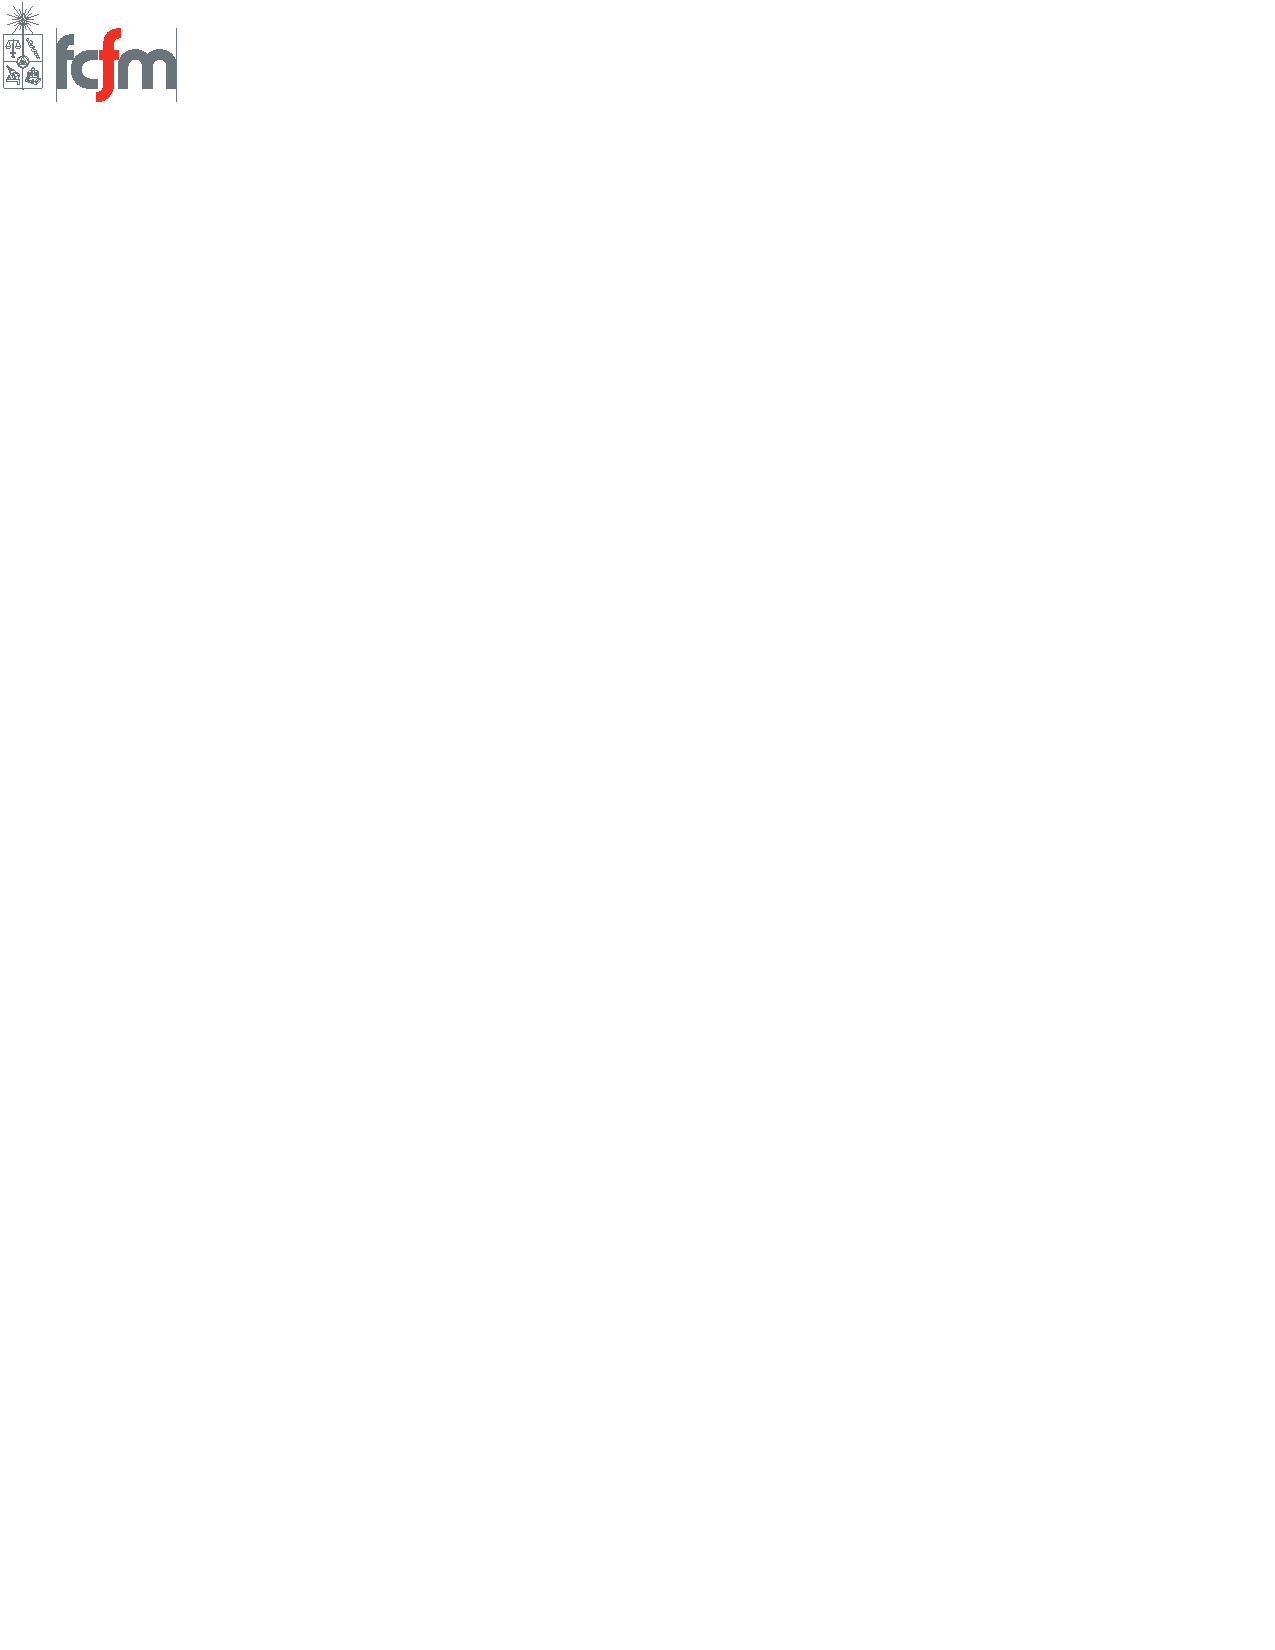
\includegraphics[scale=1.35]{departamentos/fcfm2}
	\end{wrapfigure}
	\hspace*{0.3cm}
	\noindent \textsc{\color{red} \hspace{-2.2cm} \departamentouniversidad} ~ \\
	\hspace*{0.3cm}
	\noindent \textsc{\color{dkgray} \hspace{-1.6cm} \nombrefacultad} ~ \\
	\hspace*{0.3cm}
	\noindent \textsc{\color{dkgray} \hspace{-1.6cm} \nombreuniversidad} ~ \\
	\hspace*{0.3cm}
	\noindent \textsc{\color{dkgray} \hspace{-1.6cm} \codigodelcurso \nombredelcurso} ~ \\
	\vfill
	\begin{center}
		\vspace*{0.5cm}
		{\color{dkgray} \Large \textbf{\MakeUppercase{\temaatratar}}} ~ \\
		\noindent \rule{\linewidth}{0.3mm} ~ \\
		\Huge \textup \bfseries \textsc{\textcolor{\portraittitlecolor}{\titulodelinforme}} ~ \\
		\noindent \rule{\linewidth}{0.3mm} ~ \\
	\end{center}
	\begin{minipage}{.5\textwidth}
		~
	\end{minipage}
	\vfill
	\begin{minipage}{1.0\textwidth}
		\begin{flushright}
			\noindent \tablaintegrantes
		\end{flushright}
	\end{minipage}
}{
\ifthenelse{\equal{\portraitstyle}{style7}}{
	\setpagemargincm{\pagemarginleft}{\pagemargintop}{\pagemarginright}{\pagemarginbottom}
	\thispagestyle{empty}
	\begin{center}
		\vspace*{-1.5cm}
		\includegraphics[scale=\imagendepartamentoescala]{\imagendepartamento}
		\hspace*{-0.15cm}
		\begin{tabular}{l}
			\vspace*{0.26cm}\mbox{} ~ \\
			\small \textsc{\MakeUppercase{\nombreuniversidad}} ~ \\
			\small \textsc{\MakeUppercase{\nombrefacultad}} ~ \\
			\small \textsc{\MakeUppercase{\departamentouniversidad}} ~ \\
			\vspace*{1.25cm}\mbox{}
		\end{tabular}
	\end{center}
	\vfill
	\begin{center}
		\noindent \rule{\textwidth}{0.4mm} \\ \vspace{0.3cm}
		{\huge \textcolor{\portraittitlecolor}{\titulodelinforme} \vspace{0.2cm} ~ \\}
		\noindent \rule{\textwidth}{0.4mm} ~ \\ \vspace{0.40cm}
		{\large \textcolor{\portraittitlecolor}{\temaatratar} ~ \\}
	\end{center}
	\vfill
	\noindent
	\begin{minipage}{1.0\textwidth}
		\begin{flushright}
			\scshape{\tablaintegrantes}
		\end{flushright}
	\end{minipage}
}{
\ifthenelse{\equal{\portraitstyle}{style8}}{
	\setpagemargincm{\pagemarginleft}{\pagemargintop}{\pagemarginright}{\pagemarginbottom}
	\thispagestyle{empty}
	\begin{center}
		\vspace*{-1.0cm}
		\begin{tabular}{c}
			\includegraphics[scale=\imagendepartamentoescala]{\imagendepartamento} \vspace{0.5cm} ~ \\
			\small \scshape{\MakeUppercase{\nombreuniversidad}} ~ \\
			\small \scshape{\MakeUppercase{\nombrefacultad}} ~ \\
			\small \scshape{\MakeUppercase{\departamentouniversidad}}
		\end{tabular}
	\end{center}
	\vfill
	\begin{center}
		\noindent \rule{\textwidth}{0.4mm} \\ \vspace{0.3cm}
		{\huge \textcolor{\portraittitlecolor}{\titulodelinforme} \vspace{0.2cm} ~ \\}
		\noindent \rule{\textwidth}{0.4mm} ~ \\ \vspace{0.40cm}
		{\large \textcolor{\portraittitlecolor}{\temaatratar} ~ \\}
	\end{center}
	\vfill
	\noindent
	\begin{minipage}{1.0\textwidth}
		\begin{flushright}
			\scshape{\tablaintegrantes}
		\end{flushright}
	\end{minipage}
}{
\ifthenelse{\equal{\portraitstyle}{style9}}{
	\setpagemargincm{\pagemarginleft}{\pagemargintop}{\pagemarginright}{\pagemarginbottom}
	\thispagestyle{empty}
	\noindent \includegraphics[scale=\imagendepartamentoescala]{\imagendepartamento}
	\vfill
	\begin{center}
		\noindent \rule{\textwidth}{0.4mm} \\ \vspace{0.3cm}
		{\huge \textcolor{\portraittitlecolor}{\titulodelinforme} \vspace{0.2cm} \\}
		\noindent \rule{\textwidth}{0.4mm} \\ \vspace{0.35cm}
		{\large \textcolor{\portraittitlecolor}{\temaatratar} \\}
	\end{center}
	\vfill
	\begin{center}
		\begin{tabular}{c}
			\small \scshape{\MakeUppercase{\nombreuniversidad}} ~ \\
			\small \scshape{\MakeUppercase{\nombrefacultad}} ~ \\
			\small \scshape{\MakeUppercase{\departamentouniversidad}}
		\end{tabular}
	\end{center}
	\vfill
	\begin{center}
		\indent \scshape{\tablaintegrantes}
	\end{center}
}{
\ifthenelse{\equal{\portraitstyle}{style10}}{
	\setpagemargincm{\pagemarginleft}{\pagemargintop}{\pagemarginright}{\pagemarginbottom}
	\thispagestyle{empty}
	~ \\
	\vfill
	\begin{center}
		\ifthenelse{\equal{\nombreuniversidad}{\xspace}}{
			\noindent {\large \textsc{\departamentouniversidad}}
		}{
			\noindent {\large \textsc{\nombreuniversidad, \departamentouniversidad}}
		}
		\vspace{1.0cm}
	\end{center}
	\vfill
	\begin{center}
		\noindent {\large \scshape{\nombredelcurso}} \vspace{0.5cm} ~ \\
		\noindent {\large \scshape{\codigodelcurso}} \vspace{0.5cm} ~ \\
		\noindent \rule{\textwidth}{0.4mm} \\ \vspace{0.3cm}
		{\huge \bfseries \textcolor{\portraittitlecolor}{\titulodelinforme} \vspace{0.2cm} \\}
		\noindent \rule{\textwidth}{0.4mm} \\ \vspace{2.5cm}
	\end{center}
	\vfill
	\begin{center}
		\indent \tablaintegrantes
	\end{center}
	\vfill
	~ \\
}{
\ifthenelse{\equal{\portraitstyle}{style11}}{
	\setpagemargincm{\pagemarginleft}{\pagemargintop}{\pagemarginright}{\pagemarginbottom}
	\thispagestyle{empty}
	\begin{center}
		\vspace*{-1.0cm}
		\scshape{\nombreuniversidad} ~ \\
		\scshape{\nombrefacultad} ~ \\
		\scshape{\departamentouniversidad}
	\end{center}
	\vfill
	\begin{center}
		{\setstretch{1.2} \fontsize{21pt}{22pt} \selectfont \textcolor{\portraittitlecolor}{\scshape{\titulodelinforme}} \vspace{0.5cm}} ~ \\
		{\fontsize{13pt}{10pt} \selectfont \textcolor{\portraittitlecolor}{\scshape{\temaatratar}}}
	\end{center}
	\vfill
	\begin{center}
		\indent \tablaintegrantes
	\end{center}
}{
\ifthenelse{\equal{\portraitstyle}{style12}}{
	\setpagemargincm{\pagemarginleft}{\pagemargintop}{\pagemarginright}{\pagemarginbottom}
	\thispagestyle{empty}
	\begin{center}
		\vspace*{-1.0cm}
		\includegraphics[scale=\imagendepartamentoescala]{\imagendepartamento}
	\end{center}
	\vfill
	\begin{center}
		{\bf \Huge \scshape{\textcolor{\portraittitlecolor}{\titulodelinforme}} \vspace{0.3cm}} \\
		{\bf \Large \textcolor{\portraittitlecolor}{\temaatratar}}
	\end{center}
	\vfill
	\begin{flushright}
		\noindent \tablaintegrantes
	\end{flushright}
	\vspace{0.5cm}
	\noindent \rule{\textwidth}{0.4mm}
	\begin{center}
		\ifthenelse{\equal{\nombreuniversidad}{\xspace}}{
			\scshape{\nombrefacultad} \\
		}{
			\scshape{\nombreuniversidad, \nombrefacultad} \\
		}
		\scshape{\departamentouniversidad}
	\end{center}
}{
\ifthenelse{\equal{\portraitstyle}{style13}}{
	\setpagemargincm{\pagemarginleft}{\pagemargintop}{\pagemarginright}{\pagemarginbottom}
	\thispagestyle{empty}
	\noindent
	\vspace*{-1.5cm}
	\begin{flushleft}
		\begin{minipage}{0.65\textwidth}
			\ifthenelse{\equal{\nombreuniversidad}{\xspace}}{
				{\fontsize{3.5mm}{0.5mm} \selectfont \noindent \textsf{\nombrefacultad}} ~ \\
			}{
				{\fontsize{3.5mm}{0.5mm} \selectfont \noindent \textsf{\nombreuniversidad, \nombrefacultad}} ~ \\
			}
			\noindent {\fontsize{3.0mm}{0.5mm} \selectfont \textsf{\departamentouniversidad} \vspace{-0.2cm}} ~ \\
			\noindent \textcolor{gray}{\rule{\textwidth}{0.3mm}}
		\end{minipage}
	\end{flushleft}
	\vspace*{-2.15cm}
	\begin{flushright}
		\begin{minipage}{0.3\textwidth}
			\noindent \includegraphics[width=1.0\textwidth]{\imagendepartamento}
		\end{minipage}
	\end{flushright}
	\vfill
	\begin{center}
		\begin{minipage}{0.9\textwidth}
			\begin{framed}
				\LARGE
				\vspace{1cm}
				\centering \textcolor{\portraittitlecolor}{\textbf{\titulodelinforme}}
				\vspace{1cm}
			\end{framed}
		\end{minipage}
	\end{center}
	\vfill
	\begin{flushright}
		\noindent \textsf{\tablaintegrantes}
	\end{flushright}
}{
\ifthenelse{\equal{\portraitstyle}{style14}}{
	\setpagemargincm{\pagemarginleft}{\pagemargintop}{\pagemarginright}{\pagemarginbottom}
	\thispagestyle{empty}
	\noindent
	\begin{flushleft}
		\vspace*{-1.0cm}
		\noindent \includegraphics[scale=\imagendepartamentoescala]{\imagendepartamento} \\
	\end{flushleft}
	\vfill
	{\bf \huge \noindent \textcolor{\portraittitlecolor}{\textsf{\MakeUppercase{\titulodelinforme}} \vspace*{0.05cm}}} \\
	{\bf \large \noindent \textcolor{\portraittitlecolor}{\textsf{\MakeUppercase{\temaatratar}}}} \\
	\vfill
	\begin{flushright}
		\noindent \textsf{\tablaintegrantes}
	\end{flushright}
}{
\ifthenelse{\equal{\portraitstyle}{style15}}{
	\setpagemargincm{\pagemarginleft}{\pagemargintop}{\pagemarginright}{\pagemarginbottom}
	\thispagestyle{empty}
	\checkextravarexist{\headerimageA}{Defina la imagen extra de la portada en el archivo lib/page/portrait-config.tex (VERSION NORMAL) o bien en el bloque PORTADA (VERSION COMPACTA)}
	\checkextravarexist{\headerimagescaleA}{Defina la escala de la imagen extra de la portada en el archivo lib/page/portrait-config.tex (VERSION NORMAL) o bien en el bloque PORTADA (VERSION COMPACTA)}
	\vspace*{-1.5cm}
	\noindent \begin{minipage}{0.8\textwidth}
		\noindent \begin{minipage}{0.22\textwidth}
			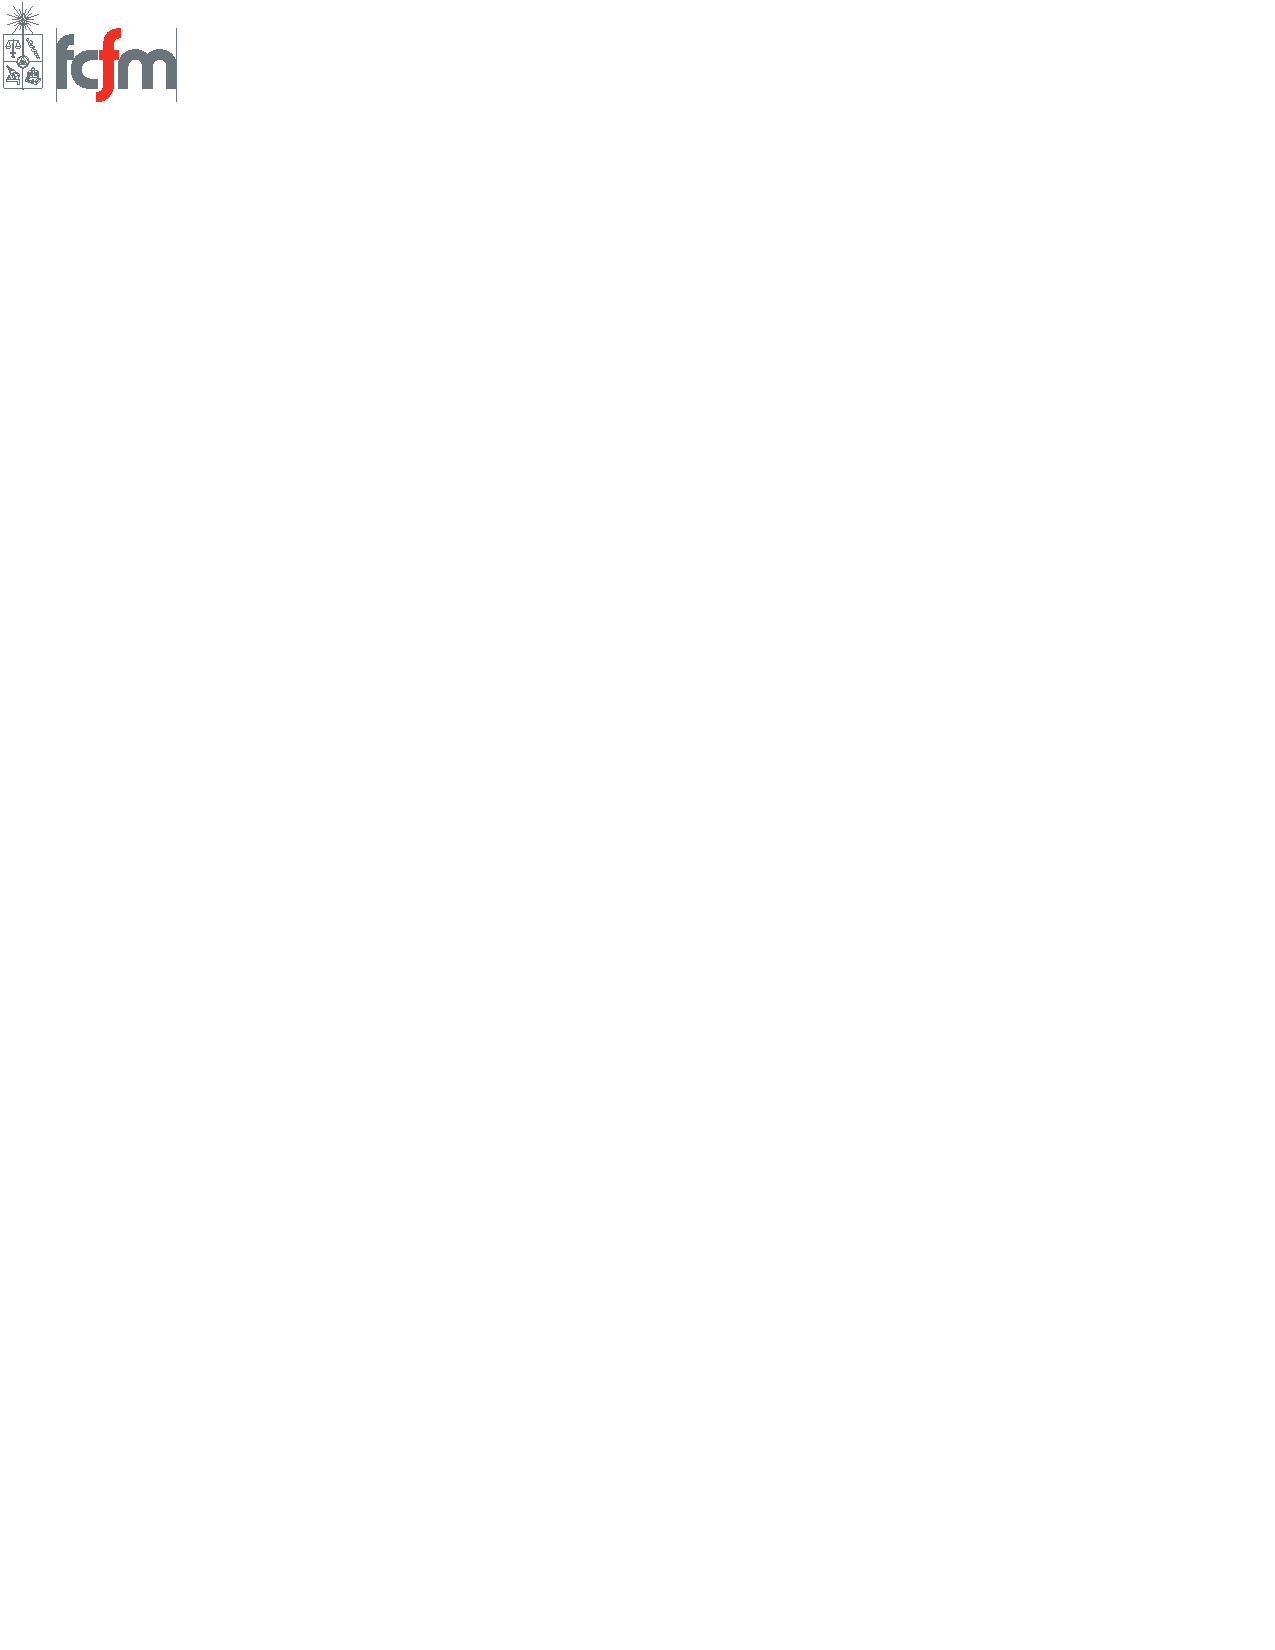
\includegraphics[scale=1.0]{departamentos/fcfm2} \\
		\end{minipage}
		\begin{minipage}{0.6\textwidth}
			\begin{flushleft}
				\textsc{
				\begin{tabular}{l}
					{\small \nombreuniversidad} ~ \\
					{\small \nombrefacultad} ~ \\
					{\small \departamentouniversidad}
				\end{tabular}
				}
			\end{flushleft}
		\end{minipage}
	\end{minipage}
	\noindent \begin{minipage}{0.2\textwidth}
		\begin{flushright}
			\ifthenelse{\isundefined{\headerimageA}}{}{
				\ifthenelse{\isundefined{\headerimagescaleA}}{}{
					\noindent \includegraphics[scale=\headerimagescaleA]{\headerimageA} \\
				}
			}
		\end{flushright}
	\end{minipage}
	\vfill
	\begin{center}
		{\fontsize{25pt}{15pt} \selectfont \textcolor{\portraittitlecolor}{\textbf{\titulodelinforme}} \vspace{0.7cm}} \\
		{\Large \textcolor{\portraittitlecolor}{\temaatratar}}
	\end{center}
	\vfill
	\begin{center}
		\noindent \tablaintegrantes
	\end{center}
}{
\ifthenelse{\equal{\portraitstyle}{style16}}{
	\setpagemargincm{\pagemarginleft}{\pagemargintop}{\pagemarginright}{\pagemarginbottom}
	\checkextravarexist{\portraitbackgroundimageB}{[portrait-style16] Defina el fondo de la portada en el archivo lib/page/portrait-config.tex (VERSION NORMAL) o bien en el bloque PORTADA (VERSION COMPACTA)}
	\checkextravarexist{\portraitbackgroundcolorB}{[portrait-style16] Defina el color del bloque del titulo de la portada en el archivo lib/page/portrait-config.tex (VERSION NORMAL) o bien en el bloque PORTADA (VERSION COMPACTA)}
	\begingroup
		\thispagestyle{empty}
		\begin{tikzpicture}[remember picture,overlay]
			\node[inner sep=0pt] (background) at (current page.center) {\includegraphics[width=\paperwidth]{\portraitbackgroundimageB}};
			\draw (current page.center) node [fill=\portraitbackgroundcolorB!30!white,fill opacity=0.6,text opacity=1,inner sep=1cm]{\Huge\centering\bfseries\sffamily\parbox[c][][t]{\paperwidth}{
					\centering \textcolor{\portraittitlecolor}{\titulodelinforme} \\ [10pt]
					{\Large \temaatratar} \\ [25pt]
					{\huge \autordeldocumento}}};
		\end{tikzpicture}
		\vfill
	\endgroup
}{
\ifthenelse{\equal{\portraitstyle}{style17}}{
	\setpagemargincm{\pagemarginleft}{\firstpagemargintop}{\pagemarginright}{\pagemarginbottom}
	\pagestyle{fancy}
	\checkextravarexist{\portraitimageC}{[portrait-style17] Defina la imagen de la portada en el archivo lib/page/portrait-config.tex (VERSION NORMAL) o bien en el bloque PORTADA (VERSION COMPACTA)}
	\checkextravarexist{\portraitimageboxedC}{[portrait-style17] Defina si la imagen de la portada se encierra en un recuadro en el archivo lib/page/portrait-config.tex (VERSION NORMAL) o bien en el bloque PORTADA (VERSION COMPACTA)}
	\checkextravarexist{\portraitimageboxedwidthC}{[portrait-style17] Defina el grosor del recuadro de la imagen de la portada en el archivo lib/page/portrait-config.tex (VERSION NORMAL) o bien en el bloque PORTADA (VERSION COMPACTA)}
	\checkextravarexist{\portraitimagewidthC}{[portrait-style17] Defina los parametros de la imagen de la portada en el archivo lib/page/portrait-config.tex (VERSION NORMAL) o bien en el bloque PORTADA (VERSION COMPACTA)}
	\fancyhf{}
	\fancyhead[L]{
		\nombreuniversidad ~ \\
		\nombrefacultad ~ \\
		\departamentouniversidad ~ \\
		\vspace{-0.43cm}
	}
	\fancyhead[R]{
		\includegraphics[scale=\imagendepartamentoescala]{\imagendepartamento}
		\hspace{-0.255cm}
	}
	~ \\
	\vfill
	\begin{center}
		\textcolor{\portraittitlecolor}{
			{\noindent \Huge{\titulodelinforme} \vspace{0.5cm}} ~ \\
			{\noindent \large{\temaatratar}}
		}
	\end{center}
	~ \\
	\ifthenelse{\equal{\portraitimageboxedC}{true}}{
		\insertimageboxed{\portraitimageC}{width=\portraitimagewidthC}{\portraitimageboxedwidthC}{}
	}{
		\insertimage{\portraitimageC}{width=\portraitimagewidthC}{}
	}
	~ \\
	\vfill
	\noindent
	\begin{minipage}{1.0\textwidth}
		\begin{flushright}
			\tablaintegrantes
		\end{flushright}
	\end{minipage}
}{
\ifthenelse{\equal{\portraitstyle}{style18}}{
	\setpagemargincm{\pagemarginleft}{\firstpagemargintop}{\pagemarginright}{\pagemarginbottom}
	\pagestyle{fancy}
	\checkextravarexist{\portraitimageD}{[portrait-style18] Defina la imagen de la portada en el archivo lib/page/portrait-config.tex (VERSION NORMAL) o bien en el bloque PORTADA (VERSION COMPACTA)}
	\checkextravarexist{\portraitimageboxedD}{[portrait-style18] Defina si la imagen de la portada se encierra en un recuadro en el archivo lib/page/portrait-config.tex (VERSION NORMAL) o bien en el bloque PORTADA (VERSION COMPACTA)}
	\checkextravarexist{\portraitimageboxedwidthD}{[portrait-style18] Defina el grosor del recuadro de la imagen de la portada en el archivo lib/page/portrait-config.tex (VERSION NORMAL) o bien en el bloque PORTADA (VERSION COMPACTA)}
	\checkextravarexist{\portraitimagewidthD}{[portrait-style18] Defina los parametros de la imagen de la portada en el archivo lib/page/portrait-config.tex (VERSION NORMAL) o bien en el bloque PORTADA (VERSION COMPACTA)}
	\fancyhf{}
	\fancyhead[L]{
		\nombreuniversidad ~ \\
		\nombrefacultad ~ \\
		\departamentouniversidad ~ \\
		\vspace{-0.43cm}
	}
	\fancyhead[R]{
		\includegraphics[scale=\imagendepartamentoescala]{\imagendepartamento}
		\hspace{-0.255cm}
	}
	~ \\
	\ifthenelse{\equal{\portraitimageboxedD}{true}}{
		\insertimageboxed{\portraitimageD}{width=\portraitimagewidthD}{\portraitimageboxedwidthD}{}
	}{
		\insertimage{\portraitimageD}{width=\portraitimagewidthD}{}
	}
	\vfill
	\begin{center}
		\textcolor{\portraittitlecolor}{
			{\noindent \Huge{\titulodelinforme} \vspace{0.5cm}} ~ \\
			{\noindent \large{\temaatratar}}
		}
	\end{center}
	\vfill
	\noindent
	\begin{minipage}{1.0\textwidth}
		\begin{flushright}
			\tablaintegrantes
		\end{flushright}
	\end{minipage}
}{
\ifthenelse{\equal{\portraitstyle}{\bgtemplatetestcode}}{
	\setpagemargincm{\pagemarginleft}{\pagemargintop}{\pagemarginright}{\pagemarginbottom}
	\pagestyle{empty}
	\pagecolor{lbrown}
	\begin{center}
		\vspace*{-1.0cm}
		\scshape{\nombreuniversidad} ~ \\
		\scshape{\nombrefacultad} ~ \\
		\scshape{\departamentouniversidad}
	\end{center}
	~ \\
	\begin{center}
		\bgtemplatetestimg
	\end{center}
	\begin{center}
		\vspace*{-6cm}
		{\setstretch{1.2} \fontsize{25pt}{22pt} \selectfont \textcolor{\portraittitlecolor}{\scshape{\titulodelinforme}} \vspace{0.5cm}} \\
		{\fontsize{15pt}{10pt} \selectfont \textcolor{\portraittitlecolor}{\scshape{\temaatratar}}}
	\end{center}
	\vfill
	\begin{flushright}
		\noindent \tablaintegrantes
	\end{flushright}
	\newpage
	\pagecolor{white}
}{
	\throwbadconfigondoc{Estilo de portada incorrecto}{\portraitstyle}{style1 .. style18}}}}}}}}}}}}}}}}}}}
}
\ifthenelse{\equal{\addemptypagetwosides}{true}}{
	\newpage
	\null
	\thispagestyle{empty}
	\renewcommand{\thepage}{}
	\newpage}{
}
 % Se puede borrar

% CONFIGURACIÓN DE PÁGINA Y ENCABEZADOS
% Template:     Informe/Reporte LaTeX
% Documento:    Configuración de página
% Versión:      6.2.2 (30/01/2019)
% Codificación: UTF-8
%
% Autor: Pablo Pizarro R. @ppizarror
%        Facultad de Ciencias Físicas y Matemáticas
%        Universidad de Chile
%        pablo.pizarro@ing.uchile.cl, ppizarror.com
%
% Manual template: [https://latex.ppizarror.com/Template-Informe/]
% Licencia MIT:    [https://opensource.org/licenses/MIT/]

\newpage
\ifthenelse{\equal{\predocuseromannumber}{true}}{
	\ifthenelse{\equal{\romanpageuppercase}{true}}{
		\pagenumbering{Roman}
	}{
		\pagenumbering{roman}
	}}{
	\pagenumbering{arabic}
}
\setcounter{page}{1}
\setcounter{footnote}{1}
\setpagemargincm{\pagemarginleft}{\pagemargintop}{\pagemarginright}{\pagemarginbottom}
\def\arraystretch {\tablepaddingv}
\setlength{\tabcolsep}{\tablepaddingh em}
\ifthenelse{\equal{\pointdecimal}{true}}{
	\decimalpoint}{
}
\renewcommand{\appendixname}{\nomltappendixsection}
\renewcommand{\appendixpagename}{\nameappendixsection}
\renewcommand{\appendixtocname}{\nameappendixsection}
\renewcommand{\contentsname}{\nomltcont}
\renewcommand{\figurename}{\nomltwfigure}
\renewcommand{\listfigurename}{\nomltfigure}
\renewcommand{\listtablename}{\nomlttable}
\renewcommand{\lstlistingname}{\nomltwsrc}
\renewcommand{\lstlistlistingname}{\nomltsrc}
\renewcommand{\refname}{\namereferences}
\renewcommand{\tablename}{\nomltwtable}
\sectionfont{\color{\titlecolor} \fontsizetitle \styletitle \selectfont}
\subsectionfont{\color{\subtitlecolor} \fontsizesubtitle \stylesubtitle \selectfont}
\subsubsectionfont{\color{\subsubtitlecolor} \fontsizesubsubtitle \stylesubsubtitle \selectfont}
\titleformat{\subsubsubsection}{\color{\ssstitlecolor} \normalfont \fontsizessstitle \stylessstitle}{\thesubsubsubsection}{1em}{}
\titlespacing*{\subsubsubsection}{0pt}{3.25ex plus 1ex minus .2ex}{1.5ex plus .2ex}
\ifthenelse{\equal{\hfstyle}{style1}}{
	\pagestyle{fancy} \fancyhf{}
	\ifthenelse{\equal{\disablehfrightmark}{false}}{
		\fancyhead[L]{\nouppercase{\rightmark}}
	}{}
	\fancyhead[R]{\small \rm \thepage}
	\fancyfoot[L]{\small \rm \textit{\titulodelinforme}}
	\fancyfoot[R]{\small \rm \textit{\codigodelcurso \nombredelcurso}}
	\renewcommand{\headrulewidth}{0.5pt}
	\renewcommand{\footrulewidth}{0.5pt}
	\renewcommand{\sectionmark}[1]{\markboth{#1}{}}
}{
\ifthenelse{\equal{\hfstyle}{style2}}{
	\pagestyle{fancy} \fancyhf{}
	\ifthenelse{\equal{\disablehfrightmark}{false}}{
		\fancyhead[L]{\nouppercase{\rightmark}}
	}{}
	\fancyhead[R]{\small \rm \thepage}
	\fancyfoot[L]{\small \rm \textit{\titulodelinforme}}
	\fancyfoot[R]{\small \rm \textit{\codigodelcurso \nombredelcurso}}
	\renewcommand{\headrulewidth}{0.5pt}
	\renewcommand{\footrulewidth}{0pt}
	\renewcommand{\sectionmark}[1]{\markboth{#1}{}}
}{
\ifthenelse{\equal{\hfstyle}{style3}}{
	\pagestyle{fancy} \fancyhf{}
	\fancyhead[L]{
		\small \rm \textit{\codigodelcurso \nombredelcurso}
		\vspace{0.04cm}
	}
	\fancyhead[R]{
		\includegraphics[width=1.2cm]{\imagendepartamento}
		\vspace{-0.10cm}
	}
	\fancyfoot[C]{\thepage}
	\renewcommand{\headrulewidth}{0.5pt}
	\renewcommand{\footrulewidth}{0pt}
}{
\ifthenelse{\equal{\hfstyle}{style4}}{
	\pagestyle{fancy} \fancyhf{}
	\ifthenelse{\equal{\disablehfrightmark}{false}}{
		\fancyhead[L]{\nouppercase{\rightmark}}
	}{}
	\fancyhead[R]{}
	\fancyfoot[C]{\small \rm \thepage}
	\renewcommand{\headrulewidth}{0.5pt}
	\renewcommand{\footrulewidth}{0pt}
	\renewcommand{\sectionmark}[1]{\markboth{#1}{}}
}{
\ifthenelse{\equal{\hfstyle}{style5}}{
	\pagestyle{fancy} \fancyhf{}
	\fancyhead[L]{\codigodelcurso \nombredelcurso}
	\ifthenelse{\equal{\disablehfrightmark}{false}}{
		\fancyhead[R]{\nouppercase{\rightmark}}
	}{}
	\fancyfoot[L]{\departamentouniversidad, \nombreuniversidad}
	\fancyfoot[R]{\small \rm \thepage}
	\renewcommand{\headrulewidth}{0pt}
	\renewcommand{\footrulewidth}{0pt}
	\renewcommand{\sectionmark}[1]{\markboth{#1}{}}
}{
\ifthenelse{\equal{\hfstyle}{style6}}{
	\pagestyle{fancy} \fancyhf{}
	\fancyfoot[L]{\departamentouniversidad}
	\fancyfoot[C]{\thepage}
	\fancyfoot[R]{\nombreuniversidad}
	\renewcommand{\headrulewidth}{0pt}
	\renewcommand{\footrulewidth}{0pt}
	\setlength{\headheight}{49pt}
}{
\ifthenelse{\equal{\hfstyle}{style7}}{
	\pagestyle{fancy} \fancyhf{}
	\fancyfoot[C]{\thepage}
	\renewcommand{\headrulewidth}{0pt}
	\renewcommand{\footrulewidth}{0pt}
	\setlength{\headheight}{49pt}
}{
\ifthenelse{\equal{\hfstyle}{style8}}{
	\pagestyle{fancy} \fancyhf{}
	\fancyfoot[R]{\thepage}
	\renewcommand{\headrulewidth}{0pt}
	\renewcommand{\footrulewidth}{0pt}
	\setlength{\headheight}{49pt}
}{
\ifthenelse{\equal{\hfstyle}{style9}}{
	\pagestyle{fancy} \fancyhf{}
	\ifthenelse{\equal{\disablehfrightmark}{false}}{
		\fancyhead[L]{\nouppercase{\rightmark}}
	}{}
	\fancyhead[R]{}
	\fancyfoot[L]{\small \rm \textit{\titulodelinforme}}
	\fancyfoot[R]{\small \rm \thepage}
	\renewcommand{\headrulewidth}{0.5pt}
	\renewcommand{\footrulewidth}{0.5pt}
	\renewcommand{\sectionmark}[1]{\markboth{#1}{}}
}{
\ifthenelse{\equal{\hfstyle}{style10}}{
	\pagestyle{fancy} \fancyhf{}
	\ifthenelse{\equal{\disablehfrightmark}{false}}{
		\fancyhead[L]{\nouppercase{\rightmark}}
	}{}
	\fancyhead[R]{\small \rm \textit{\titulodelinforme}}
	\fancyfoot[L]{}
	\fancyfoot[R]{\small \rm \thepage}
	\renewcommand{\headrulewidth}{0.5pt}
	\renewcommand{\footrulewidth}{0.5pt}
	\renewcommand{\sectionmark}[1]{\markboth{#1}{}}
}{
\ifthenelse{\equal{\hfstyle}{style11}}{
	\pagestyle{fancy} \fancyhf{}
	\ifthenelse{\equal{\disablehfrightmark}{false}}{
		\fancyhead[L]{\nouppercase{\rightmark}}
	}{}
	\fancyhead[R]{\small \rm \thepage \nomnpageof \pageref{LastPage}}
	\fancyfoot[L]{\small \rm \textit{\titulodelinforme}}
	\fancyfoot[R]{\small \rm \textit{\codigodelcurso \nombredelcurso}}
	\renewcommand{\headrulewidth}{0.5pt}
	\renewcommand{\footrulewidth}{0.5pt}
	\renewcommand{\sectionmark}[1]{\markboth{#1}{}}
}{
\ifthenelse{\equal{\hfstyle}{style12}}{
	\pagestyle{fancy} \fancyhf{}
	\fancyfoot[L]{\departamentouniversidad}
	\fancyfoot[C]{\thepage \nomnpageof \pageref{LastPage}}
	\fancyfoot[R]{\nombreuniversidad}
	\renewcommand{\headrulewidth}{0pt}
	\renewcommand{\footrulewidth}{0pt}
	\setlength{\headheight}{49pt}
}{
\ifthenelse{\equal{\hfstyle}{style13}}{
	\pagestyle{fancy} \fancyhf{}
	\fancyhead[L]{
		\small \rm \textit{\codigodelcurso \nombredelcurso}
		\vspace{0.04cm}
	}
	\fancyhead[R]{
		\includegraphics[width=1.2cm]{\imagendepartamento}
		\vspace{-0.10cm}
	}
	\fancyfoot[C]{\thepage \nomnpageof \pageref{LastPage}}
	\renewcommand{\headrulewidth}{0.5pt}
	\renewcommand{\footrulewidth}{0pt}
}{
\ifthenelse{\equal{\hfstyle}{style14}}{
	\pagestyle{fancy} \fancyhf{}
	\ifthenelse{\equal{\disablehfrightmark}{false}}{
		\fancyhead[L]{\nouppercase{\rightmark}}
	}{}
	\fancyhead[R]{}
	\fancyfoot[C]{\small \rm \thepage \nomnpageof \pageref{LastPage}}
	\renewcommand{\headrulewidth}{0.5pt}
	\renewcommand{\footrulewidth}{0pt}
	\renewcommand{\sectionmark}[1]{\markboth{#1}{}}
}{
	\throwbadconfigondoc{Estilo de header-footer incorrecto}{\hfstyle}{style1 .. style14}}}}}}}}}}}}}}
}
\ifthenelse{\equal{\showlinenumbers}{true}}{
	\linenumbers}{
}


% Template:     Informe/Reporte LaTeX
% Documento:    Índice
% Versión:      6.2.2 (30/01/2019)
% Codificación: UTF-8
%
% Autor: Pablo Pizarro R. @ppizarror
%        Facultad de Ciencias Físicas y Matemáticas
%        Universidad de Chile
%        pablo.pizarro@ing.uchile.cl, ppizarror.com
%
% Manual template: [https://latex.ppizarror.com/Template-Informe/]
% Licencia MIT:    [https://opensource.org/licenses/MIT/]

\ifthenelse{\equal{\showindex}{true}}{
	\newpage
	\begingroup
	\sectionfont{\color{\indextitlecolor} \fontsizetitlei \styletitlei \selectfont}
	\ifthenelse{\equal{\addemptypagetwosides}{true}}{
		\checkoddpage
		\ifoddpage
		\else
			\newpage
			\null
			\thispagestyle{empty}
			\newpage
			\addtocounter{page}{-1}
		\fi}{
	}
	\ifthenelse{\equal{\addindextobookmarks}{true}}{
		\belowpdfbookmark{\nomltcont}{contents}}{
	}
	\tocloftpagestyle{fancy}
	\ifthenelse{\equal{\showdotaftersnum}{true}}{
		\def\cftsecaftersnum {.}
		\def\cftsubsecaftersnum {.}
		\def\cftsubsubsecaftersnum {.}
		\def\cftsubsubsubsecaftersnum {.}
		\def\cftsecnumwidth {1.9em}
\def\cftsubsecnumwidth {2.57em}
\renewcommand\cftsubsubsecnumwidth{3.35em}
		\setlength{\cftsubsecindent}{1.91em}
\setlength{\cftsubsubsecindent}{4.48em}
		}{
	}
	\renewcommand{\cftdot}{\charnumpageindex}
	\def\cftfigaftersnum {\charafterobjectindex\enspace}
	\def\cftsubfigaftersnum {\charafterobjectindex\enspace}
	\def\cfttabaftersnum {\charafterobjectindex\enspace}
	\def\cftlstlistingaftersnum {\charafterobjectindex\enspace}
	\ifthenelse{\equal{\showlinenumbers}{true}}{
		\nolinenumbers}{
	}
	\ifthenelse{\equal{\objectindexindent}{true}}{
		\def\cftlstlistingindent {1.495em}
	}{
		\setlength{\cfttabindent}{0in}
		\setlength{\cftfigindent}{0in}
		\setlength{\cftsubfigindent}{0in}
		\setlength{\cftfigindent}{0in}
		\def\cftlstlistingindent {0.01em}
	}
	\ifthenelse{\equal{\equalmarginnumobject}{true}}{
		\ifthenelse{\equal{\showsectioncaption}{none}}{
			\def\cftdefautnumwidth {2.3em}
		}{
		\ifthenelse{\equal{\showsectioncaption}{sec}}{
			\def\cftdefautnumwidth {3.0em}
		}{
		\ifthenelse{\equal{\showsectioncaption}{ssec}}{
			\def\cftdefautnumwidth {3.7em}
		}{
		\ifthenelse{\equal{\showsectioncaption}{sssec}}{
			\def\cftdefautnumwidth {4.4em}
		}{
		\ifthenelse{\equal{\showsectioncaption}{ssssec}}{
			\def\cftdefautnumwidth {5.1em}
		}{
			\throwbadconfig{Valor configuracion incorrecto}{\showsectioncaption}{none,sec,ssec,sssec,ssssec}}}}}
		}
		\def\cftfignumwidth {\cftdefautnumwidth}
		\def\cftsubfignumwidth {\cftdefautnumwidth}
		\def\cfttabnumwidth {\cftdefautnumwidth}
		\def\cftlstlistingnumwidth {\cftdefautnumwidth}}{
	}
	\newcommand{\coregeneratefigureindex}{
		\iftotalfigures
			\ifthenelse{\equal{\indexnewpagef}{true}}{\newpage}{}
			\listoffigures
		\fi
	}
	\newcommand{\coregeneratetableindex}{
		\iftotaltables
			\ifthenelse{\equal{\indexnewpaget}{true}}{\newpage}{}
			\listoftables
		\fi
	}
	\newcommand{\coregeneratecodeindex}{
		\iftotallstlistings
			\ifthenelse{\equal{\indexnewpagec}{true}}{\newpage}{}
			\lstlistoflistings
		\fi
	}
	\ifthenelse{\equal{\showindexofcontents}{true}}{
		\tableofcontents
	}{}
	\ifthenelse{\equal{\indexstyle}{ftc}}{
		\coregeneratefigureindex
		\coregeneratetableindex
		\coregeneratecodeindex
	}{
	\ifthenelse{\equal{\indexstyle}{f}}{
		\coregeneratefigureindex
	}{
	\ifthenelse{\equal{\indexstyle}{ft}}{
		\coregeneratefigureindex
		\coregeneratetableindex
	}{
	\ifthenelse{\equal{\indexstyle}{fc}}{
		\coregeneratefigureindex
		\coregeneratecodeindex
	}{
	\ifthenelse{\equal{\indexstyle}{fct}}{
		\coregeneratefigureindex
		\coregeneratecodeindex
		\coregeneratetableindex
	}{
	\ifthenelse{\equal{\indexstyle}{t}}{
		\coregeneratetableindex
	}{
	\ifthenelse{\equal{\indexstyle}{tf}}{
		\coregeneratetableindex
		\coregeneratefigureindex
	}{
	\ifthenelse{\equal{\indexstyle}{tfc}}{
		\coregeneratetableindex
		\coregeneratefigureindex
		\coregeneratecodeindex
	}{
	\ifthenelse{\equal{\indexstyle}{tc}}{
		\coregeneratetableindex
		\coregeneratecodeindex
	}{
	\ifthenelse{\equal{\indexstyle}{tcf}}{
		\coregeneratetableindex
		\coregeneratecodeindex
		\coregeneratefigureindex
	}{
	\ifthenelse{\equal{\indexstyle}{c}}{
		\coregeneratecodeindex
	}{
	\ifthenelse{\equal{\indexstyle}{ct}}{
		\coregeneratecodeindex
		\coregeneratetableindex
	}{
	\ifthenelse{\equal{\indexstyle}{ctf}}{
		\coregeneratecodeindex
		\coregeneratetableindex
		\coregeneratefigureindex
	}{
	\ifthenelse{\equal{\indexstyle}{cf}}{
		\coregeneratecodeindex
		\coregeneratefigureindex
	}{
	\ifthenelse{\equal{\indexstyle}{cft}}{
		\coregeneratecodeindex
		\coregeneratefigureindex
		\coregeneratetableindex
	}{
	\ifthenelse{\equal{\indexstyle}{}}{
	}{
		\throwbadconfig{Estilo desconocido del indice}{\indexstyle}{,f,ft,ftc,fc,fct,t,tf,tfc,tc,tcf,c,ct,ctf,cf,cft}}}}}}}}}}}}}}}}
	}
	\endgroup
	\newpage
	\ifthenelse{\equal{\addemptypagetwosides}{true}}{
		\vfill
		\checkoddpage
		\ifoddpage
			\newpage
			\null
			\thispagestyle{empty}
			\newpage
			\addtocounter{page}{-1}
		\else
		\fi}{
	}
}{}
 % Se puede borrar

% CONFIGURACIONES FINALES
% Template:     Informe/Reporte LaTeX
% Documento:    Configuraciones finales
% Versión:      6.2.2 (30/01/2019)
% Codificación: UTF-8
%
% Autor: Pablo Pizarro R. @ppizarror
%        Facultad de Ciencias Físicas y Matemáticas
%        Universidad de Chile
%        pablo.pizarro@ing.uchile.cl, ppizarror.com
%
% Manual template: [https://latex.ppizarror.com/Template-Informe/]
% Licencia MIT:    [https://opensource.org/licenses/MIT/]

\markboth{}{}
\newpage
\ifthenelse{\equal{\disablehfrightmark}{false}}{
	\ifthenelse{\equal{\hfstyle}{style1}}{
		\fancyhead[L]{\nouppercase{\leftmark}}}{
	}
	\ifthenelse{\equal{\hfstyle}{style2}}{
		\fancyhead[L]{\nouppercase{\leftmark}}}{
	}
	\ifthenelse{\equal{\hfstyle}{style4}}{
		\fancyhead[L]{\nouppercase{\leftmark}}}{
	}
	\ifthenelse{\equal{\hfstyle}{style5}}{
		\fancyhead[R]{\nouppercase{\leftmark}}}{
	}
	\ifthenelse{\equal{\hfstyle}{style9}}{
		\fancyhead[L]{\nouppercase{\leftmark}}}{
	}
	\ifthenelse{\equal{\hfstyle}{style10}}{
		\fancyhead[L]{\nouppercase{\leftmark}}}{
	}
\ifthenelse{\equal{\hfstyle}{style11}}{
		\fancyhead[L]{\nouppercase{\leftmark}}}{
	}
\ifthenelse{\equal{\hfstyle}{style14}}{
		\fancyhead[L]{\nouppercase{\leftmark}}}{
	}}{
}
\sectionfont{\color{\titlecolor} \fontsizetitle \styletitle \selectfont}
\subsectionfont{\color{\subtitlecolor} \fontsizesubtitle \stylesubtitle \selectfont}
\subsubsectionfont{\color{\subsubtitlecolor} \fontsizesubsubtitle \stylesubsubtitle \selectfont}
\titleformat{\subsubsubsection}{\color{\ssstitlecolor} \normalfont \fontsizessstitle \stylessstitle}{\thesubsubsubsection}{1em}{}
\titlespacing*{\subsubsubsection}{0pt}{3.25ex plus 1ex minus .2ex}{1.5ex plus .2ex}
\ifthenelse{\equal{\showsectioncaption}{none}}{
}{
\ifthenelse{\equal{\showsectioncaption}{sec}}{
	\counterwithin{equation}{section}
	\counterwithin{figure}{section}
	\counterwithin{lstlisting}{section}
	\counterwithin{table}{section}
}{
\ifthenelse{\equal{\showsectioncaption}{ssec}}{
	\counterwithin{equation}{subsection}
	\counterwithin{figure}{subsection}
	\counterwithin{lstlisting}{subsection}
	\counterwithin{table}{subsection}
}{
\ifthenelse{\equal{\showsectioncaption}{sssec}}{
	\counterwithin{equation}{subsubsection}
	\counterwithin{figure}{subsubsection}
	\counterwithin{lstlisting}{subsubsection}
	\counterwithin{table}{subsubsection}
}{
\ifthenelse{\equal{\showsectioncaption}{ssssec}}{
	\counterwithin{equation}{subsubsubsection}
	\counterwithin{figure}{subsubsubsection}
	\counterwithin{lstlisting}{subsubsubsection}
	\counterwithin{table}{subsubsubsection}
}{
	\throwbadconfig{Valor configuracion incorrecto}{\showsectioncaption}{none,sec,ssec,sssec,ssssec}
}}}}}
\ifthenelse{\equal{\captionnumfigure}{arabic}}{
	\renewcommand{\thefigure}{\arabic{figure}}
}{
\ifthenelse{\equal{\captionnumfigure}{alph}}{
	\renewcommand{\thefigure}{\alph{figure}}
}{
\ifthenelse{\equal{\captionnumfigure}{Alph}}{
	\renewcommand{\thefigure}{\Alph{figure}}
}{
\ifthenelse{\equal{\captionnumfigure}{roman}}{
	\renewcommand{\thefigure}{\roman{figure}}
}{
\ifthenelse{\equal{\captionnumfigure}{Roman}}{
	\renewcommand{\thefigure}{\Roman{figure}}
}{
	\throwbadconfig{Tipo numero figura desconocido}{\captionnumfigure}{arabic,alph,Alph,roman,Roman}}}}}
}
\ifthenelse{\equal{\captionnumsubfigure}{arabic}}{
	\renewcommand{\thesubfigure}{\arabic{subfigure}}
}{
\ifthenelse{\equal{\captionnumsubfigure}{alph}}{
	\renewcommand{\thesubfigure}{\alph{subfigure}}
}{
\ifthenelse{\equal{\captionnumsubfigure}{Alph}}{
	\renewcommand{\thesubfigure}{\Alph{subfigure}}
}{
\ifthenelse{\equal{\captionnumsubfigure}{roman}}{
	\renewcommand{\thesubfigure}{\roman{subfigure}}
}{
\ifthenelse{\equal{\captionnumsubfigure}{Roman}}{
	\renewcommand{\thesubfigure}{\Roman{subfigure}}
}{
	\throwbadconfig{Tipo numero subfigura desconocido}{\captionnumsubfigure}{arabic,alph,Alph,roman,Roman}}}}}
}
\ifthenelse{\equal{\captionnumtable}{arabic}}{
	\renewcommand{\thetable}{\arabic{table}}
}{
\ifthenelse{\equal{\captionnumtable}{alph}}{
	\renewcommand{\thetable}{\alph{table}}
}{
\ifthenelse{\equal{\captionnumtable}{Alph}}{
	\renewcommand{\thetable}{\Alph{table}}
}{
\ifthenelse{\equal{\captionnumtable}{roman}}{
	\renewcommand{\thetable}{\roman{table}}
}{
\ifthenelse{\equal{\captionnumtable}{Roman}}{
	\renewcommand{\thetable}{\Roman{table}}
}{
	\throwbadconfig{Tipo numero tabla desconocido}{\captionnumtable}{arabic,alph,Alph,roman,Roman}}}}}
}
\ifthenelse{\equal{\captionnumsubtable}{arabic}}{
	\renewcommand{\thesubtable}{\arabic{subtable}}
}{
\ifthenelse{\equal{\captionnumsubtable}{alph}}{
	\renewcommand{\thesubtable}{\alph{subtable}}
}{
\ifthenelse{\equal{\captionnumsubtable}{Alph}}{
	\renewcommand{\thesubtable}{\Alph{subtable}}
}{
\ifthenelse{\equal{\captionnumsubtable}{roman}}{
	\renewcommand{\thesubtable}{\roman{subtable}}
}{
\ifthenelse{\equal{\captionnumsubtable}{Roman}}{
	\renewcommand{\thesubtable}{\Roman{subtable}}
}{
	\throwbadconfig{Tipo numero subtabla desconocido}{\captionnumsubtable}{arabic,alph,Alph,roman,Roman}}}}}
}
\ifthenelse{\equal{\captionnumcode}{arabic}}{
	\renewcommand{\thelstlisting}{\arabic{lstlisting}}
}{
\ifthenelse{\equal{\captionnumcode}{alph}}{
	\renewcommand{\thelstlisting}{\alph{lstlisting}}
}{
\ifthenelse{\equal{\captionnumcode}{Alph}}{
	\renewcommand{\thelstlisting}{\Alph{lstlisting}}
}{
\ifthenelse{\equal{\captionnumcode}{roman}}{
	\renewcommand{\thelstlisting}{\roman{lstlisting}}
}{
\ifthenelse{\equal{\captionnumcode}{Roman}}{
	\renewcommand{\thelstlisting}{\Roman{lstlisting}}
}{
	\throwbadconfig{Tipo numero codigo fuente desconocido}{\captionnumcode}{arabic,alph,Alph,roman,Roman}}}}}
}
\ifthenelse{\equal{\predocuseromannumber}{true}}{
	\renewcommand{\thepage}{\arabic{page}}}{
}
\ifthenelse{\equal{\resetpagnumafterindex}{true}}{
	\setcounter{page}{1}}{
}
\setcounter{section}{0}
\setcounter{footnote}{0}
\ifthenelse{\equal{\showlinenumbers}{true}}{
	\linenumbers}{
}


% ======================= INICIO DEL DOCUMENTO =======================

% Template:     Informe/Reporte LaTeX
% Documento:    Archivo de ejemplo
% Versión:      6.2.2 (30/01/2019)
% Codificación: UTF-8
%
% Autor: Pablo Pizarro R. @ppizarror
%        Facultad de Ciencias Físicas y Matemáticas
%        Universidad de Chile
%        pablo.pizarro@ing.uchile.cl, ppizarror.com
%
% Manual template: [https://latex.ppizarror.com/Template-Informe/]
% Licencia MIT:    [https://opensource.org/licenses/MIT/]

% ------------------------------------------------------------------------------
% NUEVA SECCIÓN
% ------------------------------------------------------------------------------
% Las secciones se inician con \section, si se quiere una sección sin número se
% pueden usar las funciones \sectionanum (sección sin número) o la función
% \sectionanumnoi para crear el mismo título sin numerar y sin aparecer en el índice.

\section{Introducción a la Ingeniería de Procesos}

    \subsection{Ingeniería de Procesos}
    
        \subsubsection{Antecedentes históricos de la Ingeniería de Procesos}
        
        Los primeros procesos nacieron de las necesidades básicas del ser humano: alimentación, abrigo, desplazamiento, etc. Por ejemplo, en alimentación, los cultivos, la conservación de los alimentos. Dentro de la conservación, utilización de sal, bebidas y alimentos fermentados. Dentro del abrigo, fabricación de tela, utilización del cuero.
        
        Originalmente, la Ingeniería Química era Ingeniería Química Industrial, la que a su vez derivaba de la Ingeniería Mecánica. Esta especialización se debío al estudio de los procesos químicos relacionados.
        
        Características de los primeros procesos incluyen:
        
        \begin{itemize}
            \item \textbf{Baja estandarización de los procesos}. Basados en lo empírico y sin control de calidad.
            \item \textbf{Baja eficiencia}.
            \item \textbf{Alto Impacto Ambiental}.
        \end{itemize}
        
            \subsubsubsection{Historia}
            
            \begin{itemize}
                \item \textbf{Siglo XVIII}: Revolución Industrial. Construcción de industrias. El desarrollo textil y la máquina de vapor.
                \item \textbf{1887}: \textbf{George E. Davis} (University of Manchester) el primero que se conoce en realizar cursos de Ingeniería de Procesos.
                \item \textbf{1888}: En el MIT, se crea la carrera de Ingeniería Química.
                \item \textbf{1901}: Primer manual de IQ escrito por George E. Davis.
                \item \textbf{1908}: se crea la primera asocación \textbf{American Institute Chemical Engineers}.
                \item \textbf{1916}: \textbf{Arthur D. Little} (MIT) acuña el concepto de \textbf{Operaciones Unitarias}.
                \item \textbf{1919}: Primera carrera de IQ en Chile, en la \textbf{Universidad de Concepción}.
            \end{itemize}
            
            \newpage
            
            \subsubsubsection{Definición de Ingeniería Química}
            
            Según AIChe (\textit{American Institute Chemical Engineers}):
            
            \begin{quote}
                \textit{\say{Ingeniería Química es la profesión en la cual el conocimiento de la matemática, química y otras ciencias básicas, ganados por el estudio, la experiencia y la práctica, es aplicado con juicio para desarrollar maneras económicas de usar materiales y energía para el beneficio de la humanidad.}}
            \end{quote}
            
            Según Universidad Nacional de Tucumán, Argentina:
            
            \begin{quote}
                \textit{\say{Rama de la Ingeniería que se dedica al estudio, síntesis, desarrollo, diseño, operación y optimización de todos aquellos procesos industriales que producen cambios físicos, químicos y/o bioquímicos en los materiales para beneficio de la humanidad.}}
            \end{quote}
        
        \subsubsection{Rol del une ingeniere de procesos}
        
        Tareas de un Ingenierio de Procesos:
        
        \begin{multicols}{2}
            \begin{enumerate}
                \item Estudios de factibilidad técnico económica.
                \item Diseño de equipos y procesos.
                \item Construcción/Montaje de equipos y plantas
                \item Control de Producción/Operación de Plantas Industriales
                \item Control de Calidad de Productos
                \item Compras y Comercialización
                \item Ventas Técnicas
                \item Control Ambiental
                \item Investigación y Desarrollo de nuevos Productos y Procesos (innovación)
                \item Gerencia y Administración
                \item Capacitación de Recursos Humanos
            \end{enumerate}
        \end{multicols}
        
        \subsubsection{Campo Ocupacional}
        
        Campo Laboral:
        
        \begin{multicols}{2}
            \begin{enumerate}
                \item Plantas industriales
                \item Empresas de construcción y/o montaje de plantas y equipos
                \item Empresas proveedoras de servicios técnicos (consultoría, control de calidad, mantenimiento, etc.)
                \item Organismos gubernamentales o no gubernamentales de acreditación, control y estándares
                \item Instituciones de educación superior
                \item Centros de Investigación y Desarrollo (Industriales/Académicos)
            \end{enumerate}
        \end{multicols}
        
        Sectores Industriales:
        
        \begin{multicols}{2}
            \begin{enumerate}
                \item Industria Minera
                \item Industria Textil
                \item Industria Química ej. Detergentes, pinturas, adhesivos
                \item Alimentos y Bebidas
                \item Siderúrgica/Metalúrgica
                \item Industria Biotecnólogica (farmacéuticas, biopolímeros, etc.)
                \item Industria sanitaria
                \item Materiales/Polímeros/Plásticos
                \item Petroquímica/Refinerías
                \item Generación de energía
            \end{enumerate}
        \end{multicols}
        
        \subsubsection{Ética profesional}
        
        Código de Ética AIChE:
        
        \begin{quote}
            \textit{\say{Defender y avanzar en la integridad, honor y dignidad de la profesión de la ingeniería mediante: ser honesto e imparcial y servir con fidelidad a sus empleades, clientes, y al público; esforzarse en aumetar la competencia y prestigio de la profesión ingenieril; y usar su conocimiento y habilidad para mejorar el bienestar humano.}}\footnote{Traducción libre}
        \end{quote}
        
        Desafíos de la disciplina
        
        \begin{multicols}{2}
            \begin{enumerate}
                \item Cambio de escala
                \item Manejo de la energía
                \item Nuevos materiales
                \item Nuevos (bio)productos
                \item Sustentabilidad
                \item Economía circular
            \end{enumerate}
        \end{multicols}
        
        Ley de \textbf{Responsabilidad Extendida del Productor} (REP):
        
        \begin{quote}
            \textit{\say{La industria debe responsabilizarse por sus productos a través de la prevención de generación de residuos y de su recuperación y reciclaje}}
        \end{quote}
        
        A partir del 16 de marzo 2021 comenzó a regir una nueva etapa de la Ley \textbf{REP}, que establece que para 2034 las empresas deberán recolectar los residuos de envases y embalajes de 80\% de las viviendas del país.
        
        \subsubsection{Ejemplos de procesos químicos y biotecnológicos: Producción de celulosa Kraft}
        
        Chile exporta 2 millones de toneladas anuales de celulosa.
        
        \insertimagerightline[\label{fig:celulosa}]{esquemas/celulosa.png}{0.2}{3}{Molécula de celulosa}
    
        Celulosa: \textit{\say{nombre genérico para un amplio rango de productos compuestos por fibras naturales, contenido principalmente en árboles y plantas. Biopolímero de glucosa (\textbf{Figura \ref{fig:celulosa}}) con enlaces \(\beta\;1-4\) presente comúnmente en plantas.}}
        \newline
        
        Etapas de producción:
        
        \begin{enumerate}
            \item \textbf{Preparación de la madera y cocción}: Dependiendo del proceso se puede optar por varias materias primas, en este caso serán chips de madera. Estructuras vegetales contienen otros compuestos además de celulosa, como la lignina. La primera etapa consiste en realizar una cocción mediante digestión con sulfuro de sodio (\(N_{2}S\)) e hidróxido de sodio (\(NaOH\)) a \(150{}^{o}C\), con esto ocurre la ruptura de la lignina. La lignina se elimina en forma de licor negro, el cual puede ser reciclado.
            \item \textbf{Blanqueo ECF}: Existen varias formas de blaqueo, en ester caso se usa Blanqueo \textit{Elemental Chlorine Free} (ECL), es decir, que no existe cloro elemental disponible, lo que genera menos contaminación. Este procesos elimina más lignina mediante digestión con dióxido de cloro, oxígeno y peróxido de hidrógeno (\(H_{2}O_{2}\)). Se intenta reciclar lo más posible.
            \item \textbf{Secado y embalado}: Secado de la fibra, pasa a ser de \(1-2\%\) fibra a \(89-92\%\) fibra. Se obtiene una pasta de celulosa la cual se compacta a pliegos en fardos (\(250 [kg]\) o rollos de celulosa.
            \item \textbf{Recuperación y energía}: Subproductos pueden ser utilizados. Corteza, aserrines y astillas se aprovechan en calderas, como combustible. Compuestos inorgánicos se recuperan y reutilizan, o son tratados previo a desecharse. Del licor negro que se recupera se puede obtener metanol, tall oil y trementina, el resto va a la caldera. Se obtienen también, del licor negro, fitosteroles que son añadidos a alimentos, los cuales compiten con la absorción de colesterol.
            \item \textbf{Tratamiento de efluentes}: Tratamiento de aguas para eliminar los contaminantes antes de ser desechados. Tratamiento primario, remoción de sólidos, en esta primera etapa se utilizan filtros o decantadores. Tratamiento secundario, reducción de DBO (Demanda Bioquímica de Oxígeno), que es un índice de la cantidad de matera orgánica en el efluente. En esta etapa, se utilizan consorcios microbianos que se alimentan de los compuestos biológicos en el agua.
            \item \textbf{Control de emisiones}: Eliminación de emisiones gaseosa, por lo general, a altas temperaturas. Procesos que se utilizan dependen del tipo particular. Se pueden utilizar filtros o procesos de lavado de gases. Los sólidos que se pueden quemar son usados como combustible. Algunos sólidos pueden ser peligrosos los cuales son tratados por empresas externas.
        \end{enumerate}
    
    \subsection{Conceptos Básicos, Procesos y Representación}
    
    Etapas de Síntesis de Proceso:
    
    \begin{multicols}{2}
        \begin{itemize}
            \item Ingeniería de producto (\textit{¿Qué hacer?})
            \item Ingeniería de diseño (\textit{¿Cómo hacerlo?})
            \item Impacto Ambiental
            \item Rentabilidad
        \end{itemize}
    \end{multicols}
    
    Para ello:
    
    \begin{enumerate}
        \item Se define el problema (materias primas, producto, requerimientos)
        \item Selección de proceso y variables de operación
        \item Análisis de la solución obtenida
    \end{enumerate}
    
        \subsubsection{Materias Primas}
        
        \begin{itemize}
            \item \textbf{Productos agrícolas, ganaderos y forestales}: frutas, vegetales, animales, madera.
            \item \textbf{Agua}: reactivo, solvente.
            \item \textbf{Minerales}: química inorgánica
            \item \textbf{Combustibles fósiles}: gas natural, petróleo, carbón.
            \item \textbf{Gases}: Aire oxígeno, nitrógeno, \(CO_{2}\)
        \end{itemize}
        
        \subsubsection{Restricciones y funciones objetivo}
        
        Objetivo de producción:
        
        \begin{multicols}{2}
            \begin{itemize}
                \item Maximizar la producción
                \item Minimizar los costos
                \item Maximizar la calidad
                \item Maximizar la seguridad
                \item Minimizar los impactos ambientales
                \item Minimizar el uso de recursos
            \end{itemize}
        \end{multicols}
        
        Consideraciones:
        
        \begin{multicols}{2}
            \begin{itemize}
                \item Disponibilidad de las materias primas
                \item Factor económico, ambiental y social
                \item Seguridad del producto
                \item Comercialización, patentes, tecnología
            \end{itemize}
        \end{multicols}
    
        \subsubsection{Proceso, Operaciones y Variables}
        
        \textbf{Proceso}:
            
        \begin{quote}
            \textit{\say{Conjunto o secuencia de operaciones unitarias que modifican una materia prima para transformarla en un producto comercial o insumo.}}
        \end{quote}
        
        \textbf{Operación unitaria}:
        
        \begin{quote}
            \textit{\say{Etapa de un proceso donde se realiza una modificación específica (ej. destilación, molienda, evaporación, etc).}}
        \end{quote}
        
        \textbf{Modos de Operación Unitaria}
        
        \begin{itemize}
            \item \textbf{Batch}:
            \begin{quote}
                \textit{\say{Es un proceso que sucede a través de cargas, es decir, existe un periodo de carga, operación, descarga y limpieza por separado Por lo anterior, posee una cantidad inicial limitada de materia prima. Ejemplo cotidiano: Hervir agua.}}
            \end{quote}
            
            \item \textbf{Continuo}:
            \begin{quote}
                \textit{\say{Es un proceso que ocurre, como su nombre lo indica, de forma continua, es decir, existe un flujo entrante en todo momento, al igual que un flujo de salida NO es necesario que la magnitud de estos flujos sean iguales. Ejemplo (\textit{no tan}) cotidiano: Represas}}
            \end{quote}
        \end{itemize}
        
        \textbf{Variable}:
        
        \begin{quote}
            \textit{\say{moles, masa, composición, concentración, presión, temperatura, volumen, densidad, velocidad de flujo (y energía).}}
        \end{quote}
        
        \subsubsection{Diagramas}
        
        Representación compacta y precisa de un proceso. Contiene gran cantidad de información técnica.
        
            \subsubsubsection{Diagramas de Entrada-Salida}
            
            Un solo bloque representa todas las operaciones involucrada en el proceso. Se indican: materias primas, reacción estequiométrica (si existe) y productos (\textbf{Figura \ref{fig:diag-e-s}}). Flechas indican movimientos de materiales. Ejemplo en \textbf{Figura \ref{fig:diag-e-s_ej}}, producción de amoniaco (\(NH_{3}\)).
            
            \begin{figure}
                \centering
                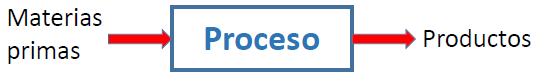
\includegraphics[width=.6\textwidth]{img/esquemas/diagrama_e-s.png}
                \caption{Diagrama de Entrada-Salida}
                \label{fig:diag-e-s}
            \end{figure}
            
            \begin{figure}
                \centering
                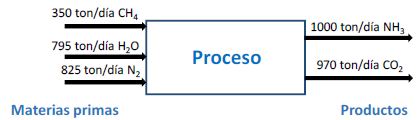
\includegraphics[width=.6\textwidth]{img/esquemas/diagrama_e-s_ej.png}
                \caption{Ejemplo de diagrama de Entrada-Salida}
                \label{fig:diag-e-s_ej}
            \end{figure}
            
            \subsubsubsection{Diagramas de Bloques}
            
            Representación \textbf{esquemática} del proceso, donde se ilustran sus características esenciales (\textbf{Figura \ref{fig:diag_bloq_ej}}, ejemplo producción de amoniaco, \(NH_{3}\)):
            
            \begin{itemize}
                \item Secuencia en que ocurren las operaciones unitarias
                \item Equipos utilizados para realizar cada operación
                \item Flujos de materia y energía
            \end{itemize}
            
            Ejemplos de unidades de proceso:
            
            \begin{itemize}
                \item \textbf{Mezclador}: Combina entradas en una salida.
                \item \textbf{Reactor}: Reactivos a la entrada reaccionan para dar productos de salida.
                \item \textbf{Divisor}: Divide entrada en múltiples salidas de igual composición.
                \item \textbf{Separador}: Divide entrada en múltiples salidas de composiciones diferentes.
            \end{itemize}
            
            \begin{figure}
                \centering
                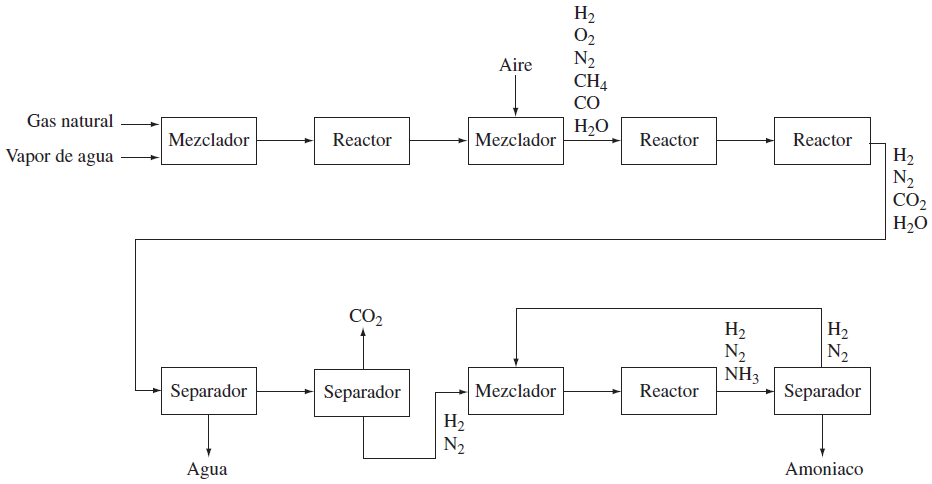
\includegraphics[width=.8\textwidth]{img/esquemas/diagrama_bloq_ej.png}
                \caption[Ejemplo de Diagrama de Bloques]{Ejemplo de Diagrama de Bloques para el procesos de producción de amoniaco (\(NH_{3}\)) \cite{murphy_introduction_2007}.}
                \label{fig:diag_bloq_ej}
            \end{figure}
            
            \subsubsubsection{Diagramas de Flujo de Proceso}
            
            Representación más cercana a la realidad. Se representan equipos por medio de símbolos (\textbf{Figura \ref{fig:diag_flux_equip}}). Interrelación entre equipos por medio de líneas de unión (Ejemplo en \textbf{Figura \ref{fig:diag_flux_ej}}).
            
            \begin{figure}
                \centering
                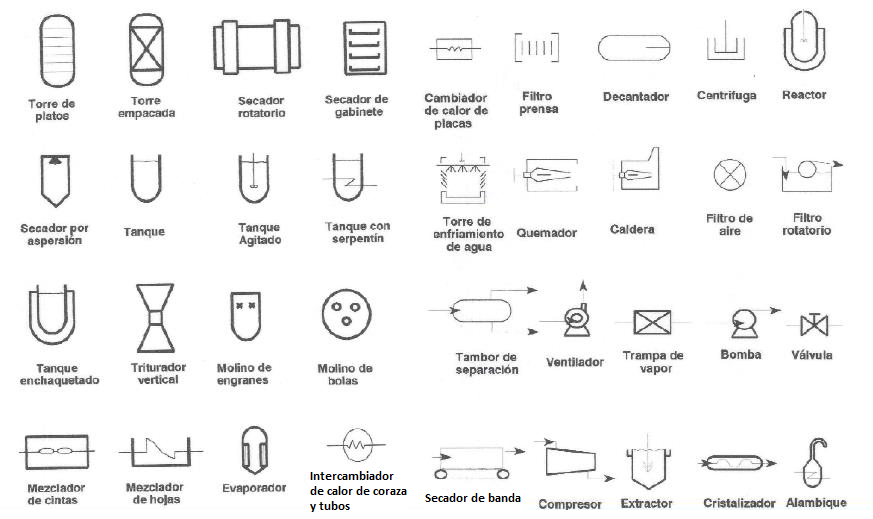
\includegraphics[width=\textwidth]{img/esquemas/diagrama_flux_equip.png}
                \caption{Esquemas de equipos para un diagrama de procesos}
                \label{fig:diag_flux_equip}
            \end{figure}
            
            Las propiedades físicas, las cantidades, las temperaturas y las presiones de los materiales, entre otros, se pueden indicar de las siguientes formas:
            \begin{enumerate}
                \item Colocando los datos sobre cada corriente.
                \item Identificando la corriente con un número o letra que refiera una lista adjunta.
                \item Adjuntando los datos en una hoja de tabulación.
            \end{enumerate}
            
            \begin{figure}
                \centering
                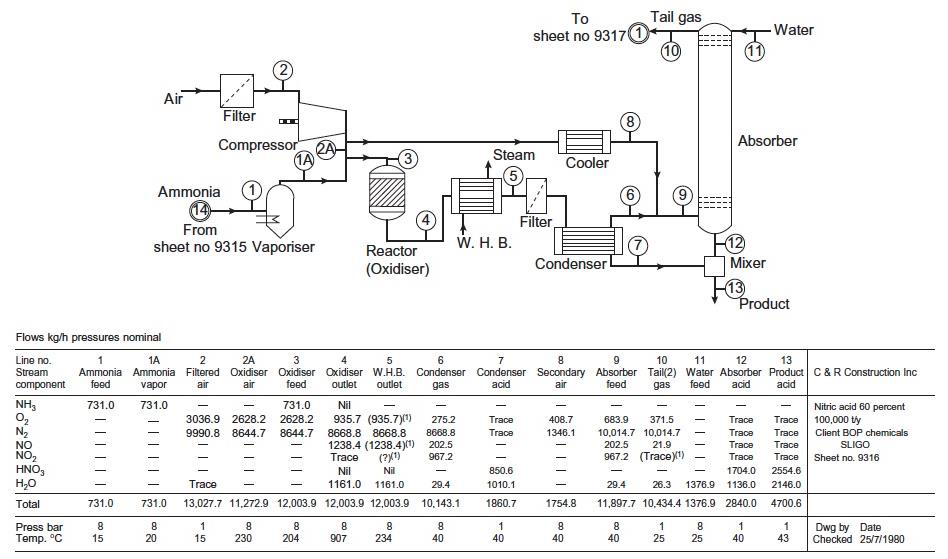
\includegraphics[width=\textwidth]{img/esquemas/diagrama_flux_ej.png}
                \caption[Ejemplo diagrama de flujo de procesos]{Ejemplo diagrama de flujo de procesos para la producción de amoniaco (\(NH_{3}\)) \cite{towler_chemical_2013}.}
                \label{fig:diag_flux_ej}
            \end{figure}
            
            Muy utilizados en la Ingeniería Química debido a:
            
            \begin{enumerate}
                \item Ayudan al diseño y organización de la planta
                \item Describen el proceso
                \item Facilitan el dimensionamiento de equipos
                \item Sirven como medio de instrucción para el personal
                \item Ayudan a la realización de balances de masa y energía
            \end{enumerate}
            
        \subsubsection{Corrientes de un Proceso}
        
        Flujos de materia que ingresan (alimentación) o salen (producto) de una operación unitaria o equipo. Formadas por una o varias sustancias o compuestos químicos. Formadas por una o más fases (por ejemplo, sólido en suspensión en un líquido). Una corriente se caracteriza por su composición, su presión y su temperatura.
        
            \subsubsubsection{Concepto de Flujo en Procesos Continuos}
            
            Un flujo corresponde a una cantidad de materia/energía que está pasando a través de un área transversal en una unidad de tiempo.
            
            El flujo puede estar compuesto de tantas especies como se estén transportando Para distinguirlas usaremos el concepto composición de flujo (\(x_{i}\)), que indica la fracción del flujo que corresponde a la especie \(i\).
            \begin{multicols}{2}
                \[\sum_{i} x_{i}^{F_{j}} = 1\]
                
                \[\sum_{i} \left ( x_{i}^{F_{j}} \cdot F_{j} \right ) = F_{j}\]
            \end{multicols}
        
        \subsubsection{Cantidades y Unidades SI}
        
        Una dimensión es cualquier cantidad medible (tiempo, longitud, velocidad, masa, ...)
        
            \subsubsubsection{Cantidad primaria}
            
            Dimensión particular para la cual ha sido definida una escala \textbf{arbitraria} de medición (unidad) (\textbf{Tabla \ref{tab:unid_prim}}).
            
            \begin{table}[H]
                \centering
                \resizebox{\textwidth}{!}{
                    \begin{tabular}{|l|c|c|c|c|c|}
                        \hline
                        \textbf{Magnitud física básica} & \multicolumn{1}{l|}{\textbf{Símbolo}} & \multicolumn{1}{l|}{\textbf{Unidad básica}} & \multicolumn{1}{l|}{\textbf{Símbolo}} & \multicolumn{1}{l|}{\textbf{Unidad cgs}} & \multicolumn{1}{l|}{\textbf{Símbolo}} \\ \hline
                        Tiempo & T & segundo & s & segundo & s \\
                        Longitud & L & metro & m & centímetro & cm \\
                        Masa & M & kilogramo & kg & gramo & g \\
                        Corriente eléctrica & I & amperio & A & estatamperio & statA \\
                        Temperatura termodinámica & \(\Theta\) & kelvin & K & kelvin & K \\
                        Cantidad de Sustancia & N & mol & mol & mol & mol \\
                        Intensidad luminosa & J & candela & cd & - & - \\ \hline
                    \end{tabular}
                }
                \caption{Cantidades primarias y su unidad de medida}
                \label{tab:unid_prim}
            \end{table}
        
            \subsubsubsection{Cantidad secundaria}
            
            Dimensión que se expresa en términos de cantidades primarias a través de leyes físicas. Ejemplo: volumen, presión, velocidad.
        
        \subsubsection{Reacciones químicas}
        
            \subsubsubsection{Ecuaciones balanceadas}
        
            \begin{itemize}
                \item \textbf{\(\nu_{i}\)}: Coeficiente estequiométrico. Reactantes se definen negativos, productor positivos.
                \item \textbf{\(\epsilon_{hi}\)}: Átomos de \(h\) en el compuesto \(i\).
                \item Ecuación balanceada:
                \[\sum_{i} \epsilon_{hi}\nu_{i} = 0\]
            \end{itemize}
            
            \textbf{Ejemplo}:
            
            Ecuación no balanceada:
            \[NH_{3} + O_{2} \rightarrow HNO_{3} + H_{2}O\]
            
            Sistema de ecuaciones, una ecuación por cada elemento:
            \[
            \begin{matrix}
                N: & 1\nu_{NH_{3}} & + & 0\nu_{O_{2}} & + & 1\nu_{HNO_{3}} & + & 0\nu_{H_{2}O} & = & 0 \\
                H: & 3\nu_{NH_{3}} & + & 0\nu_{O_{2}} & + & 1\nu_{HNO_{3}} & + & 2\nu_{H_{2}O} & = & 0 \\
                O: & 0\nu_{NH_{3}} & + & 2\nu_{O_{2}} & + & 3\nu_{HNO_{3}} & + & 1\nu_{H_{2}O} & = & 0
            \end{matrix}
            \]
            Solución:
            \[\nu_{NH_{3}} = -1 \wedge \nu_{O_{2}} = -2 \wedge \nu_{HNO_{3}} = 1 \wedge \nu_{H_{2}O} = 1\]
            
            Ecuación balanceada:
            \[NH_{3} + 2O_{2} \rightarrow HNO_{3} + H_{2}O\]
            
            \subsubsubsection{Análisis generación consumo}
            
            Cálculo de materias primas, productos y subproductos con reacciones múltiples. Para ello:
            
            \begin{enumerate}
                \item Escribir las \(k\) reacciones balanceadas
                \item Listar reactivos y compuestos asociando su respectivo \(\nu_{ik}\), \(i\) compuesto y \(k\) reacción.
                \item Calcular:
                \[\nu_{i,neto} = \sum_{k} \nu_{ik}\]
            \end{enumerate}
            
            Ejemplo:
            \[
            \begin{matrix}
                R_{1} & CH_{4} & + & H_{2}O & \rightarrow & CO + 3H_{2} \\
                R_{2} & CO & + & H_{2}O & \rightarrow & CO_{2} + H_{2} \\
                R_{3} & N_{2} & + & 3H_{2} & \rightarrow & 2NH_{3}
            \end{matrix}
            \]
            
            \begin{table}[H]
                \centering
                \begin{tabular}{l c c c c}
                    \hline
                    \textbf{Compuesto} & \begin{tabular}[c]{@{}l@{}}\(R_{1}\) \\ \(\nu_{i1}\)\end{tabular} & \begin{tabular}[c]{@{}l@{}}\(R_{2}\) \\ \(\nu_{i2}\)\end{tabular} & \begin{tabular}[c]{@{}l@{}}\(R_{3}\) \\ \(\nu_{i3}\)\end{tabular} & \begin{tabular}[c]{@{}l@{}} \textbf{Neto} \\ \(\nu_{i,neto}\)\end{tabular} \\ \hline
                    \(CH_{4}\) & \(-1\) &  &  & \(-1\) \\
                    \(H_{2}O\) & \(-1\) & \(-1\) &  & \(-2\) \\
                    \(CO\) & \(+1\) & \(-1\) &  & \(0\) \\
                    \(H_{2}\) & \(+3\) & \(+1\) & \(-3\) & \(+1\) \\
                    \(CO_{2}\) &  & \(+1\) &  & \(+1\) \\
                    \(N_{2}\) &  &  & \(-1\) & \(-1\) \\
                    \(NH_{3}\) &  &  & \(+2\) & \(+2\) \\ \hline
                \end{tabular}
                \caption{Ejemplo de análisis generación consumo}
                \label{tab:ex_gen_consumo}
            \end{table}
            
            Ecuación proceso neto:
            
            \[CH_{4} + 2H_{2}O + N_{2} \rightarrow H_{2} + CO_{2} + 2NH_{3}\]
            
            \subsubsubsection{Masa, Moles y Masa Molar}
            
            \textbf{Masa molar}:
            
            \begin{quote}
                \textit{\say{masa en gramos de un \(mol\) de átomos o moléculas.}}
            \end{quote}
            
            \[1 [mol] = 6.02 \cdot 10^{23} \text{ átomos o moléculas}\]
            
            \begin{multicols}{2}
                \textbf{Conversión}:
            
                \[MM = \frac{n}{m}\]
                
                Con \(n\) moles y \(m\) masa en gramos.
                
                Para pasar de masa a moles:
                \[n = MM \cdot m\]
                
                Para pasar de moles a masa:
                \[m = \frac{n}{MM}\]
            \end{multicols}
            
            \subsubsubsection{Composición de una corriente}
            
            \begin{multicols}{2}
                \textbf{Fracción másica}
            
                \[W_{i} = \frac{m_{i}}{m_{\text{Total}}}\]
                
                \textbf{Fracción molar}
                
                \[x_{i} = \frac{n_{i}}{n_{\text{Total}}}\]
                
                Fracciones deben sumar 1.
                \[W_{i} \neq x_{i}\]
                
                \textbf{Partes por millón (\(ppm\))}
                
                \[ppm = x_{i} \cdot 10^{6}\]
                
                \textbf{Razón de composición}
                
                \textbf{Razón másica}
                
                \[W_{i,j} = \frac{m_{i}}{m_{j}}\]
                
                \textbf{Razón molar}
                
                \[x_{i,j} = \frac{n_{i}}{n_{j}}\]
            \end{multicols}

\section{Balances de Masa en Estado Estacionario}

    \subsection{Análisis de grados de Libertad}
    
        \subsubsection{Ley de conservación de la materia}
        
        Ley de Lomonósov-Lavosier (Siglo XVIII) (de conservación de la materia):
        
        \begin{quote}
            \textit{\say{Nada se crea ni se destruye, sólo se transforma. La materia no se crea ni se destruye durante una reacción química, sólo se transforma.}}
        \end{quote}
        
        \subsubsection{Balance de Masa para procesos en Estado Estacionario}
        
            \subsubsubsection{Balance de Masa}
            
            Ley de conservación de la masa se aplica en procesos químicos sin reacción nuclear. Se deben definir claramente los límites del sistema (\textbf{Figura \ref{fig:balance_masa_esq}}).
            
            \begin{figure}
                \centering
                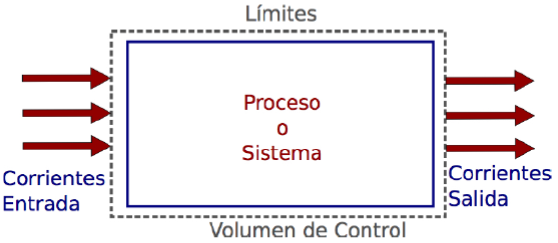
\includegraphics[width=.7\textwidth]{img/esquemas/balance_masa_esq.png}
                \caption{Esquema del balance de masa sobre un volumen de control de límites definidos}
                \label{fig:balance_masa_esq}
            \end{figure}
            
            Solo interesan las corrientes que cruzan los límites del sistema:
            \begin{equation}
            \label{eq:balance_masa}
                \text{Flujo entrada} - \text{Flujo salida} + \text{Generación} - \text{Consumo} = \text{Acumulación}
            \end{equation}
            
            El balance de masa se puede aplicar a:
            
            \begin{enumerate}
                \begin{minipage}{0.2\linewidth}
                    \item Masa total
                    \item Moles totales
                \end{minipage}
                \begin{minipage}{0.4\linewidth}
                    \item Masa o moles de cada especie
                    \item Masa o moles de átomos
                \end{minipage}
                \begin{minipage}{0.3\linewidth}
                    \item Operación unitaria o equipo
                    \item Proceso completo.
                \end{minipage}
            \end{enumerate}
            
            El sistema puede estar compuesto de una o varias operaciones unitarias (ejemplo en \textbf{Figura \ref{fig:balance_masa_ej}}.
            
            \begin{figure}
                \centering
                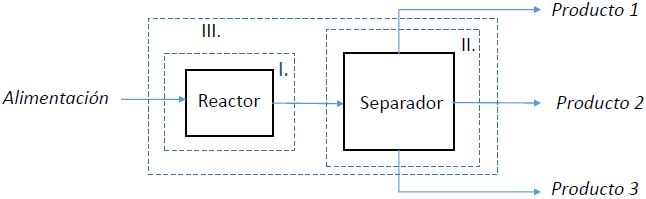
\includegraphics[width=.9\textwidth]{img/esquemas/balance_masa_ej.png}
                \caption[Ejemplo de balance de masa]{Ejemplo de balance de masa sobre un reactor (I), sobre el separador (II), o sobre ambas operaciones unitarias (III)}
                \label{fig:balance_masa_ej}
            \end{figure}
            
            \subsubsubsection{Proceso en Estado Estacionario}
            
            \textbf{Estado Estacionario (SS, \textit{Steady State})}:
            
            Todas las variables del proceso son independientes del tiempo (\(T, P, F, x_{i}\)). El término de acumulación en la ecuación de balance de masa (\textbf{Ecuación \ref{eq:balance_masa}}) es nulo (\textbf{Ecuación \ref{eq:balance_masa_esta}}). Esta situación en la práctica se da en procesos continuos en régimen estacionario.
            
            \begin{equation}
            \label{eq:balance_masa_esta}
                \text{Flujo entrada} - \text{Flujo salida} + \text{Generación} - \text{Consumo} = 0
            \end{equation}
            
            \textbf{Estado Transiente (NOSS, \textit{NOn-Steady State})}:
            
            Corresponde al estado en que un proceso (y por ende, todas sus operaciones unitarias) o una operación unitaria en particular varía en el tiempo. El balance se transforma en una ecuación diferencial a resolver.
            \[\frac{d(\cdot)}{dt} = \text{Flujo entrada} - \text{Flujo salida} + \text{Generación} - \text{Consumo}\]
        
        \subsubsection{Análisis de Grados de libertad (\(N_{L}\))}
        
        Sirve para predecir si habrá una solución completa a un problema de análisis de proceso, sin resolver el problema.
        
        \begin{equation}
        \label{eq:grados_libertad}
            \left \| N_{L} = N_{V} - N_{R} \right \| 
        \end{equation}
        
        Con \(N_{L}\) grados de libertad del sistema, \(N_{V}\) número de variables del sistema y \(N_{R}\) número de restricciones del sistema.
        
        \begin{itemize}
            \item \(\mathbf{N_{L} = 0}\): el sistema está totalmente \textbf{definido} (determinado) y se pueden calcular las incógnitas.
            \item \(\mathbf{N_{L} < 0}\): el sistema está \textbf{sobredeterminado}.
            \item \(\mathbf{N_{L} > 0}\): el sistema está \textbf{subdeterminado}, se deben definir variables para obtener una única solución al problema.
        \end{itemize}
        
            \subsubsubsection{Número de variables (\(N_{V}\))}
            
            Variables asociadas a \underline{una corriente} con \(N_{SP}\) especies:
            
            \begin{itemize}
                \begin{minipage}{0.45\linewidth}
                    \item Flujo (\(F_{i}\))
                    \item Composición (\(y_{i}\), líquida. \(x_{i}\), gaseosa)
                \end{minipage}
                \begin{minipage}{0.25\linewidth}
                    \item Presión (\(P_{i}\))
                    \item Temperatura (\(T_{i}\))
                \end{minipage}
                \begin{minipage}{0.2\linewidth}
                    \item Entalpía (\(H_{i}\))
                    \newline
                    \newline
                \end{minipage}
            \end{itemize}
            
            Por cada corriente se tendría \(N_{V}\):
            \begin{equation}
                \label{eq:nv_1}
                \left \| N_{SP} + 4 \right \|\text{, ya que}\;N_{SP}\rightarrow \text{composiciones}\wedge4\rightarrow F_{i}, P_{i}, T_{i}, H_{i}
            \end{equation}
            
            Pero no todas las variables son independientes, ya que:
            \[\sum_{i}^{N_{SP}} Y_{i} = 1 \wedge H_{i} = f(Y_{i}, P_{i}, T_{i})\]
            
            Por lo que a \textbf{Ecuación \ref{eq:nv_1}} se le debe restar 2. Teniendo un \(N_{V}\) por corriente:
            \begin{equation}
            \label{eq:nv_2}
                N_{SP} + 2
            \end{equation}
            
            Para un sistema con \(N_{C}\) corrientes queda:
            \[\overset{\text{\textbf{Ecuación \ref{eq:nv_2}}} \cdot N_{C}}{\Rightarrow} N_{C}\left ( N_{SP} + 2 \right ) \overset{+\text{Balance de energía}}{\Rightarrow}\]
            \begin{equation}
            \label{variables_por_corriente}
                \left \| N_{V} = N_{C}\left ( N_{SP} + 2 \right ) + 1 \right \|
            \end{equation}
            
            \subsubsubsection{Número de restricciones (\(N_{R}\))}
            
            \begin{enumerate}
                \item \textbf{Composiciones cero}, cuando no existe entrada/salida de una especie (\(\max({N_{SP} - 1})\) por corriente).
                \item \textbf{Composiciones conocidas} (\(\max({N_{SP} - 1})\) por corriente)
                \item \textbf{Balance de masa independientes}
                \begin{itemize}
                    \item Si no hay reacción química:
                    \[N_{BM_{indep}} = N_{SP}\]
                    
                    \item Si hay reacción química:
                    \[N_{BM_{indep}} = N_{SP} - N_{rxn\;indep}\]
                \end{itemize}
                Para calcular el número de reacciones químicas independientes (\(N_{rxn\;indep}\)), se calcula el rango de la matriz atómica.
                \textbf{Matrix atómica}
                
                \[
                \begin{matrix}
                     & SP_{1} & \cdots & SP_{n} \\
                    \begin{array}{c}
                        EL_{1} \\
                        \cdots \\
                        EL_{m}
                    \end{array} & \left (
                    \begin{array}{c}
                        \cdots \\
                        \vdots \\
                        \cdots
                    \end{array} \right . &
                    \begin{array}{c}
                        \cdots \\
                        \ddots \\
                        \cdots
                    \end{array} & \left .
                    \begin{array}{c}
                        \cdots \\
                        \vdots \\
                        \cdots
                    \end{array} \right )
                \end{matrix}
                \]
                
                Con \(SP_{i}\) la especie y \(EL_{j}\) el elemento.
                \[N_{rxn\;indep} = N_{SP} - \text{rango de la matriz, con}\]
                \[\text{rango de la matriz} = N_{Balances}\]
                \item \textbf{Balance de energía} (el sistema completo: \(1\))
                \item \textbf{Datos conocidos}:
                \begin{multicols}{3}
                    \begin{enumerate}
                        \item Presión
                        \item Temperatura
                        \item Conversión
                        \item Rendimiento
                        \item Exceso
                        \item ...
                    \end{enumerate}
                \end{multicols}
                \item \textbf{Identidad de composición}. En un divisor de flujo, cada salida tiene la misma composición en cada salida, solo divide el flujo.
                
                Número de restricciones del sistema debido a identidad de composición \(N_{R(IC)}\).
                \[N_{R(IC)} = (N_{J} - 1 )(N_{SP} - 1)\]
                
                Con \(N_{J}\) número de corrientes de salida.
            \end{enumerate}
        
        \subsubsection{Grados de Libertad del Sistema Integrado}
        
        Si se considera el sistema completo (global), se consideran solo las corrientes de entrada y salida del sistema. En cambio, si se considera cada subsistema (integrado), se consideran las corrientes de conexión. Se calculan, entonces, las restricciones por corrientes de conexión.
        \[N_{L} = \sum_{i} {N_{L}}_{i} - \sum_{j} {N_{C}}_{j}\]
        
        Con \({N_{L}}_{i}\) grados de libertad del subsistema \(i\), \({N_{C}}_{j}\) variables en corrientes de conexión \(j\)
        
        \[{N_{C}}_{j} = {N_{C}}_{\text{en conexión}} + (N_{SP} - 1) - \text{Data en corriente}\]
        
        \begin{quote}
            \textit{\say{Los grados de libertad del sistema integrado son distintos de los grados de libertad del sistema global.}}
        \end{quote}
        
        Esto se debe a que al realizar el análisis integrado, se consideran las variables de las conexiones del sistema.
    
    \subsection{Balance de Masa sin reacción química}
    
        \subsubsection{Planteamiento}
        
        \begin{enumerate}
            \item Dibuja diagrama del proceso.
            \item Identificar los componentes y definir las variables de cada corriente.
            \item Colocar información conocida en el diagrama (ej: Flujos, especies, composiciones, \(T\), \(P\), etc) en unidades congruentes (ej: masa, moles).
            \textit{Recomendación:}
            \begin{itemize}
                \item Líquidos y sólidos: en masa.
                \item Gases: en moles.
            \end{itemize}
            \item Defina un sistema.
            \item Si existen reacciones químicas de estequiometría conocida, escribir ecuación que relacione el consumo de reactivos con la generación de productos.
            \item Determinar el número de incógnitas y balances independientes.
            \item Escribir un conjunto apropiado de balances para resolver el problema.
            \item Definir base de cálculo y resolver las ecuaciones en unidades consistentes.
            \item Verificar la solución (ej. Flujos \(\geq 0\); composiciones \(0 \leq x_{i} \leq 1\)).
        \end{enumerate}
        
        \subsubsection{Sin reacción}
        
        \begin{itemize}
            \item La masa se conseva.
            \item Los moles se conservan si no hay reacción.
            \item Sistema \underline{sin reacciones químicas}, el número de balances de masa independientes es igual al número de especies.
        \end{itemize}
        
        Desde \textbf{Ecuación \ref{eq:balance_masa_esta}}:
        \[\text{Flujo entrada} - \text{Flujo salida} + \cancelto{0}{\text{Generación}} - \cancelto{0}{\text{Consumo}} = 0 \Rightarrow\]
        \begin{equation}
        \label{eq:balance_masa_esta_sin}
            \text{Flujo entrada} = \text{Flujo salida}
        \end{equation}
        
        
        
        \subsubsubsection{Múltiples Sistemas}
        
        \begin{itemize}
            \item Para cada sistema, se pueden plantear tantos balances de masa como especies haya en el sistema.
            \item Los balances de masa del sistema global son dependientes de los balances de masa de los subsistemas.
        \end{itemize}
    
    \subsection{Balance de Masa sin y con reacción química}
    
    \begin{itemize}
        \item La masa se conserva.
        \item Todas las variables del proceso son independientes del tiempo (\(T\), \(P\), \(F\), \(X_{i}\), \(\dots\)).
        \item El término de acumulación del BM (Balance de Masas) es nulo (cero)
    \end{itemize}
    
    \textbf{Ecuación \ref{eq:balance_masa_esta}}:
    \[\text{Flujo entrada} - \text{Flujo salida} + \text{Generación} - \text{Consumo} = 0\]
    
        \subsubsection{Conceptos}
        
        \[a A + b B \rightarrow c C + d D\]
        
            \subsubsubsection{Condiciones estequiométricas}
            
            \begin{quote}
                \textit{\say{Si se hacen reaccionar \(a\) moles de \(A\) con \(b\) moles del reactante \(B\).}}
            \end{quote}
        
            \subsubsubsection{Condiciones no estequiométricas}
            
            \begin{quote}
                \textit{\say{Si se hacen reaccionar \(a\) moles de \(A\) con \(f\) moles del reactante \(B\), donde \(f \neq b\).}}
            \end{quote}
            
            \subsubsubsection{Cuocientes estequiométrico}
            
            \begin{quote}
                \textit{\say{En una reacción balanceada, es la razón entre los coeficientes estequiométricos de dos especies que participan en la reacción.}}
            \end{quote}
            
            \[\text{Cuociente estequiométrico} = \frac{b}{a}\]
            
            \subsubsubsection{Reactivo limitante}
            
            \begin{quote}
                \textit{\say{Es el reactivo que se termina primero, cuando esto ocurre se detiene la reacción. Se calcula en base a la estequiometría de la reacción.}}
            \end{quote}
            
            \subsubsubsection{Reactivo en exceso}
            
            \begin{quote}
                \textit{\say{Todos los reactivos distintos al reactivo limitante; el exceso se calcula en base a la cantidad de reactivo limitante alimentado y la estequiometría de la reacción.}}
            \end{quote}
            
            \subsubsubsection{Exceso (\(e\))}
            
            \begin{equation}
            \label{eq:exceso}
                \begin{matrix}
                     e = \frac{n - n_{d}}{n_{d}} & & & \%e = \frac{n - n_{d}}{n_{d}} \cdot 100
                \end{matrix}
            \end{equation}
            
            Con \(n\) cantidad presente del reactivo en exceso y \(n_{d}\) cantidad estequiométrica requerida según el reactivo limitante.
            
            Si se agregan \(a\) moles de \(A\) y \(f\) moles de \(B\), donde \(f > b\):
            \[\frac{f}{a} > \frac{b}{a} \Rightarrow
            \begin{matrix}
                 B\text{: reactivo en exceso} \\
                 A\text{: reactivo limitante}
            \end{matrix}
            \Rightarrow \%e = \frac{f - b}{b} \cdot 100
            \]
            
            \subsubsubsection{Conversión (\(\alpha\))}
            
            \begin{quote}
                \textit{\say{Es la fracción del reactivo limitante que reacciona.}}
            \end{quote}
            
            \[\alpha = \frac{\text{moles de reactivo limitante que reaccionan}}{\text{moles iniciales de reactivo limitante}}\]
            \[0 \leq \alpha \leq 1\]
            \[\alpha = 1 \Rightarrow \text{Conversión total}\]
    
    \subsection{Balance de Masa con reacción química}
    
    \textbf{Rendimiento \(R\)}:
    \begin{quote}
        \textit{\say{Es la razón entre los moles (o masa) de reactivo convertido en producto deseado y los moles (o masa) de reactivo alimentado.}}
    \end{quote}
    \[R = \frac{\text{moles (masa) reactivo convertido al producto deseado}}{\text{moles (masa) de reactivo alimentado}}\]
    \newpage
    
    \textbf{Selectividad \(S\)}:
    \begin{quote}
        \textit{\say{Es la razón entre los moles de un reactivo (limitante) consumido para generación del producto de interés y los moles de reactivo consumido por todas las reacciones que ocurren.}}
    \end{quote}
    \[S = \frac{\text{moles reactivos convertido al producto deseado}}{\text{moles totales de reactivo limitante que reaccionan}} = \frac{R}{\alpha}\]
    
        \subsubsection{Conceptos}
        
            \subsubsubsection{Reciclo}
            
            \insertimagerightline[\label{fig:reciclo}]{esquemas/reciclo.png}{0.3}{5}{Reciclo}
            
            Una corriente de reciclo es una corriente que devuelve parte del material de una corriente de salida de una unidad a una corriente de entrada de esta misma unidad o de otra unidad anterior en la secuencia de proceso.
            
            El objetivo del reciclo es ajustar las condiciones de la corriente de salida, reutilizar material o aumentar la conversión en un proceso con reacción química, recirculando reactante (valioso) no reaccionado. \newline
            
            \textbf{Reciclo con reacción}:
            
            \begin{figure}
                \centering
                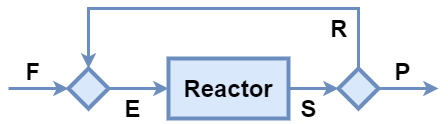
\includegraphics[width=.5\textwidth]{img/esquemas/reciclo_reaccion.png}
                \caption{Reciclo con reacción}
                \label{fig:reciclo_rxn}
            \end{figure}
            
            \begin{multicols}{2}
                \begin{itemize}
                    \item \textbf{F}: Alimentación (fresca) al proceso.
                    \item \textbf{E}: Alimentación al reactor.
                    \item \textbf{S}: Salida del reactor.
                    \item \textbf{R}: Reciclo.
                    \item \textbf{P}: Salida del proceso.
                \end{itemize}
            \end{multicols}
            
            En este caso es importante distinguir la \textbf{conversión global} (\(\alpha_{G}\)) alcanzada en el procesos global de la \textbf{conversión por pasada} (\(\alpha_{1}\)) en el reactor.
            
            \[
            \begin{matrix}
                 \alpha_{G} = \frac{(F\cdot Y_{F}) - P \cdot Y_{P}}{F \cdot Y_{F}} & & & \alpha_{1} = \frac{(E\cdot Y_{E}) - S \cdot Y_{S}}{E \cdot Y_{E}}
            \end{matrix}
            \]
            
            \[
            \begin{matrix}
                 E = F + R & | & S = R + P & | &\alpha_{G} \geq \alpha_{1}
            \end{matrix}
            \]\newline
            
            \subsubsubsection{Bypass}
            
            \insertimageleftline[\label{fig:bypass}]{esquemas/bypass.png}{0.3}{6}{Bypass}
            
            Una corriente de bypass es aquella que salta una etapa (o más) del proceso y va directamente a una etapa posterior.
            
            Se utiliza para controlar o variar la composición de una corriente de salida de una unidad. Esto se logra mezclando la corriente de bypass con la corriente de salida en proporciones adecuadas.
            
            \insertimagerightline[\label{fig:purga}]{esquemas/purga.png}{0.3}{5}{Purga}
            
            La corriente bypass permite reducir el volumen tratado en el proceso y así reducir el tamaño de los equipos.
            
            \subsubsubsection{Purga}
            
            Una corriente de purga es aquella que, en un proceso con reciclo, sale del sistema para evitar la acumulación de inertes o materiales indeseables asociados a la corriente de reciclo.
    
    \subsection{Balance de Masa con Equilibrio}
    
    \begin{itemize}
        \item El equilibrio de una reacción provee un comportamiento límite para el proceso.
        \item La reacción no procede hasta conversión completa.
        \item Cada condición de equilibrio entrega relaciones de composición adicionales a los balances de masa.
        \item El equilibrio termodinámico se aplica siempre a la corriente de salida del reactor, que debe estar en equilibrio.
        \item Un error típico consiste en mezclar en el cálculo del equilibrio componentes de la corriente de entrada (no necesariamente en equilibrio) y de la corriente de salida.
    \end{itemize}
    
        \subsubsection{Constante de Equilibrio}
        
        La constante de equilibrio indica la relación que deben tener los reactantes y productos entre sí, una vez alcanzada la condición de equilibrio. La constante de equilibrio puede ser expresada en función de presiones parciales (\(K_{P}\)) o concentraciones molares (\(K_{C}\)) y su valor depende de la temperatura de operación.
        \begin{equation}
        \label{eq:k_c}
            \alpha_{1} A_{1} + \alpha_{2} A_{2} + \cdots \rightleftharpoons \beta_{1} B_{1} + \beta_{2} B_{2} + \cdots \Rightarrow K_{C} = \frac{\prod_{\text{Productos}} A_{i}^{\alpha_{i}}}{\prod_{\text{Reactantes}} B_{i}^{\beta_{i}}}
        \end{equation}
        
        \begin{equation}
        \label{eq:k_c_pressure}
            K_{P} = \frac{\prod_{\text{Productos}} \left ( y_{A_{i}} \cdot P_{T} \right )^{\alpha_{i}}}{\prod_{\text{Reactantes}} \left ( y_{B_{i}} \cdot P_{T} \right )^{\beta_{i}}}
        \end{equation}
        
        Ejemplo:
        \begin{multicols}{2}
            Con presiones:
            \[\alpha A + \beta B \rightleftharpoons \gamma C + \delta D\]
            \[K_{P} = \frac{\left ( y_{C} \cdot P_{T}\right )^{\gamma} \cdot \left ( y_{D} \cdot P_{T}\right )^{\delta}}{\left ( y_{A} \cdot P_{T}\right )^{\alpha} \cdot \left ( y_{B} \cdot P_{T}\right )^{\beta}}\]
            
            Con concentraciones
            \[e E + f F \rightleftharpoons g G + h H\]
            \[K_{C} = \frac{\left [ G \right ]^{g} \cdot \left [ H \right ]^{h}}{\left [ E \right ]^{e} \cdot \left [ F \right ]^{f}}\]
        \end{multicols}
        
        Para gases ideales:
        \begin{equation}
        \label{eq:k_c_gases_id}
            K_{P} = K_{C} \cdot \left ( RT\right )^{\Delta n}
        \end{equation}
        
        Con \(\Delta n = \text{moles de productos} - \text{moles de reactantes}\).
        
        Para diferentes temperaturas, se utiliza la ecuación de van't Hoff:
        \begin{equation}
        \label{eq:vant_hoff}
            \ln{\frac{K_{2}}{K_{1}}} = - \frac{\Delta H^{o}}{R} \left ( \frac{1}{T_{2}} - \frac{1}{T_{1}} \right )
        \end{equation}
        
        Con \(K_{i}\) constante de equilibrio a temperatura absoluta \(T_{i}\), \(\Delta H^{o}\) variación de la entalpía en condiciones estándar y \(R\) constante de los gases.
    
    \subsection{Balance en Sistemas de una fase}
    
        \subsubsection{Conceptos}
        
        \textbf{Propiedad}:
        
        \begin{quote}
            \textit{\say{característica medible (o calculable) de una sustancia.}}
        \end{quote}
        
        \textbf{Estado}:
        
        \begin{quote}
            \textit{\say{Un sistema se encuentra en un cierto estado cuando posee un conjunto único de propiedades (ej. \(P\), \(T\), \(r\)) en un momento dado.}}
        \end{quote}
        
        \textbf{Equilibrio}:
        
        \begin{quote}
            \textit{\say{Estado en que no existe tendencia alguna al cambio.}}
        \end{quote}
        
        \textbf{Fase}:
        
        \begin{quote}
            \textit{\say{Estado de la materia completamente homogéneo y uniforme.}}
        \end{quote}
        
        \textbf{Gas Ideal}:
        
        \begin{quote}
            \textit{\say{Un gas se considera ideal cuando la distancia entre las moléculas permite ignorar el efecto de las fuerzas intermoleculares y el volumen de las moléculas mismas.}}
        \end{quote}
    
        \subsubsection{Gas ideal}
        
        \begin{figure}
            \centering
            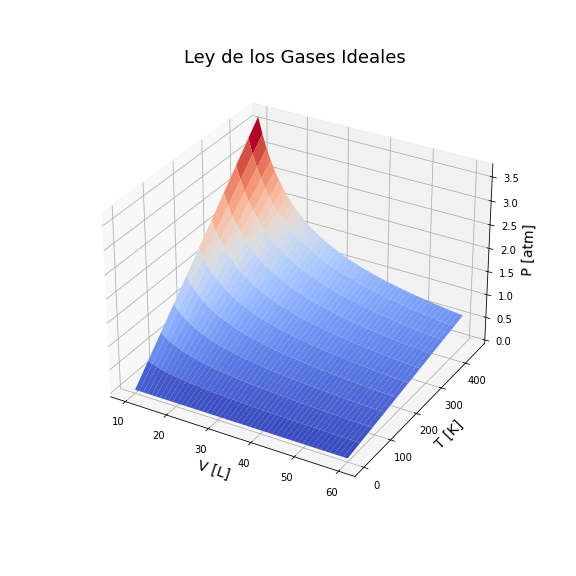
\includegraphics[width=.8\textwidth]{img/graficos/ley_gases.png}
            \caption{Ley de los Gases Ideales}
            \label{fig:gas_ideal}
        \end{figure}
        
        \begin{equation}
        \label{eq:gas_ideal}
            PV = nRT
        \end{equation}
        \newpage
        
        \textbf{Ley de Boyle-Mariotte}:
        
        \begin{minipage}{0.5\linewidth}
            \begin{figure}
               \centering
               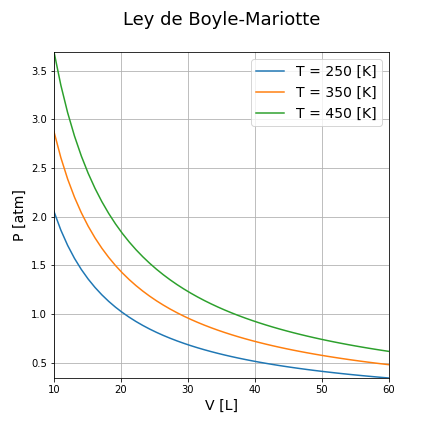
\includegraphics[width=\textwidth]{img/graficos/ley_boyle_mariotte.png}
               \caption{Ley de Boyle-Mariotte}
               \label{fig:pv}
            \end{figure}
        \end{minipage}
        \begin{minipage}{0.4\linewidth}
            \[P \cdot V = cte\]
            \[\frac{P_{2}}{P_{1}} = \frac{V_{1}}{V_{2}}\]
        \end{minipage}
        \newline
        
        \textbf{Ley de Charles}:
        
        \begin{minipage}{0.4\linewidth}
            \[\frac{T}{V} = cte\]
            \[\frac{T_{2}}{T_{1}} = \frac{V_{2}}{V_{1}}\]
        \end{minipage}
        \begin{minipage}{0.5\linewidth}
            \begin{figure}
                \centering
                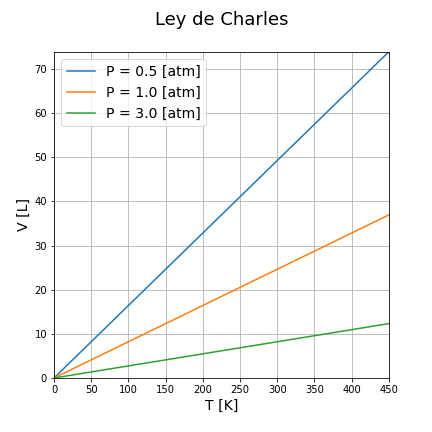
\includegraphics[width=\textwidth]{img/graficos/ley_charles.png}
                \caption{Ley de Charles}
                \label{fig:tv}
            \end{figure}
        \end{minipage}
        \newline
        \newpage
        
        \textbf{Ley de Gay-Lussac}
        
        \begin{minipage}{0.5\linewidth}
            \begin{figure}
                \centering
                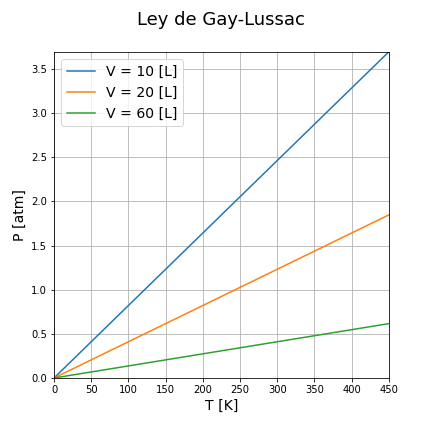
\includegraphics[width=\textwidth]{img/graficos/ley_gay_lussac.png}
                \caption{Ley de Gay-Lussac}
                \label{fig:pt}
            \end{figure}
        \end{minipage}
        \begin{minipage}{0.4\linewidth}
            \[\frac{P}{T} = cte\]
            \[\frac{P_{2}}{P_{1}} = \frac{T_{2}}{T_{1}}\]
        \end{minipage}
    
            \subsubsubsection{Condiciones Normales y Estándar}
            
            \textbf{Condiciones normales}:
            \[\left \| T = 25 [{}^{o}C] = 298.15 [K] \right \| \;\;  \left \| P = 1 [atm] = 101.325 [kPa] \right \|\]
            
            \textbf{Condiciones Estándar}:
            
            \begin{center}
                \textbf{IUPAC}\footnote{IUPAC: International Union of Pure and Applied Chemistry (\href{https://iupac.org/}{\textit{website}})}: \(\left \| T = 0 [{}^{o}C] = 273.15 [K] \right \| \;\;  \left \| P = 100 [kPa] = 0.986 [atm] = 1 [bar] = 14.504 [psi]  \right \|\)
                
                \textbf{NIST}\footnote{NIST: National Institute of Standards and Technology (\href{https://www.nist.gov/}{\textit{website}})}: \(\left \| T = 20 [{}^{o}C] = 293.15 [K] \right \| \;\;  \left \| P = 101.325 [kPa] = 1 [atm] = 14.696 [psi]  \right \|\)
            \end{center}
        
        \subsubsection{Definiciones}
            
        \textbf{Densidad de un gas (\(\rho\))}:
        
        \begin{quote}
            \say{\textit{Masa por unidad de volumen} \( \left ( \left [ \frac{kg}{m^{3}} \right ], \left [ \frac{lb}{{pie}^{3}} \right ], \left [ \frac{g}{L} \right ], \text{etc}, \cdots \right )\). \textit{La masa contenida en un volumen unitario varía con la temperatura y la presión.}}
        \end{quote}
        
        \begin{equation}
        \label{eq:rho}
            \rho = \frac{n \cdot P \cdot M}{V}
        \end{equation}
        
        Con \(M\), masa del gas.
        \newline
        
        \textbf{Peso específico relativo de un gas (\({p.e.r.}_{gas}\))}:
        
        \begin{quote}
            \say{\textit{Razón entre la densidad del gas a \(P\) y \(T\) deseadas y la del aire (o un gas de referencia) a una cierta presión y temperatura.}}
        \end{quote}
        
        \begin{equation}
        \label{eq:per_gas}
            {p.e.r.}_{gas} = \frac{\rho_{gas}(S.C.)}{\rho_{aire}(S.C.)}
        \end{equation}
        
        \textbf{Escala de Temperatura}
        
        \begin{multicols}{2}
            \[\Delta T \left [ {}^{o}F \right ] = \Delta T \left [ R \right ]\]
            
            \[\frac{\Delta T \left [ {}^{o}C \right ]}{\Delta T \left [ {}^{o}F \right ]} = 1.8\]
            
            \[T \left [ K \right ] = T \left [ {}^{o}C \right ] + 273.15\]
            
            \[\Delta T \left [ {}^{o}C \right ] = \Delta T \left [ K \right ]\]
            
            \[\frac{\Delta T \left [ K \right ]}{\Delta T \left [ R \right ]} = 1.8\]
            
            \[T \left [ R \right ] = T \left [ {}^{o}F \right ] + 460\]
            
        \end{multicols}
        
        \textbf{Mezcla de gases ideales}
        
        \begin{quote}
            \say{\textit{La presión parcial de un gas \(i\) es una cantidad ficticia que corresponde a la presión que ejercería un sólo componente de la mezcla gaseosa si ocupara el mismo volumen que ocupa la mezcla, a la misma temperatura de la mezcla.}}
        \end{quote}
        
        \[{P}_{T}{V}_{T} = n_{T}R{T}_{T} \wedge {P}_{i}{V}_{T} = n_{i}R{T}_{T} \Rightarrow {P}_{i} = \frac{n_{i}}{n_{T}} P_{T} \Rightarrow\]
        \begin{equation}
        \label{eq:p_parcial}
            P_{i} = y_{i} P_{T}
        \end{equation}
        
        Con \(y_{i}\) fracción molar del componente \(i\).
        
        \[P_{1} + P_{2} + \cdots + P_{n} = \sum_{i=1}^{n} P_{i} = P_{T}\]
    
    \subsection{Balances en sistema de Una o Varias Fases}
    
        \subsubsection{Gases reales}
        
        \begin{quote}
            \textit{\say{Los valores de las propiedades de algunos gases en condiciones normales y a alta presión se desvían del comportamiento ideal.}}
        \end{quote}
        
            \subsubsubsection{Factor de comprensibilidad (\(z\))}
            
            \begin{equation}
            \label{eq:factor_compres}
                z = \frac{PV}{nRT} = \frac{P\widehat{V}}{RT}
            \end{equation}
            
            Con \(\widehat{V} = \frac{V}{n}\) volumen molar.
            
        \subsubsection{Ley de los Estados Correspondientes}
            
            \subsubsubsection{Estado crítico}
            
            \begin{quote}
                \textit{\say{Para una transición de fase (gas\(\rightarrow\)líquido), es el conjunto de condiciones físicas en que la densidad de ambas fases se hacen idénticas.}}
            \end{quote}
            
            \subsubsubsection{Fluido supercrítico}
            
            \begin{quote}
                \textit{\say{Es un compuesto en un estado por encima del punto crítico y combina algunas de las propiedades de los gases y los líquidos.}}
            \end{quote}
            
            \subsubsubsection{Diagrama PVT agua}
            
            \begin{figure}
                \centering
                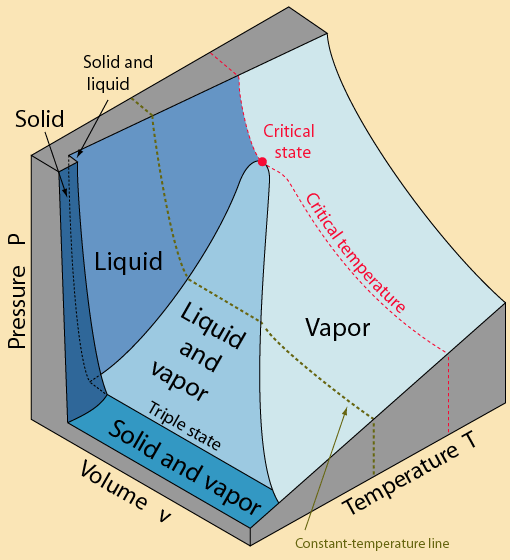
\includegraphics[width=.55\textwidth]{img/diagramas/pvtexp.png}
                \caption[Diagrama PVT de una sustancia que se expande al enfriarse]{Diagrama PVT de una sustancia que se expande al enfriarse \cite{nave_pvt_2017}}
                \label{fig:pvt_agua}
            \end{figure}
            
            \subsubsubsection{Parámetros reducidos}
            
            \begin{multicols}{3}
                \[T_{r} = \frac{T}{T_{C}}\]
                
                \[P_{r} = \frac{P}{P_{C}}\]
                
                \[V_{r} = \frac{\widehat{V}}{\widehat{V_{C}}}\]
                
            \end{multicols}
            
            \[\Rightarrow V_{r} = \frac{\widehat{V}{P}_{C}}{R{T}_{C}}\]
            
            \begin{figure}
                \centering
                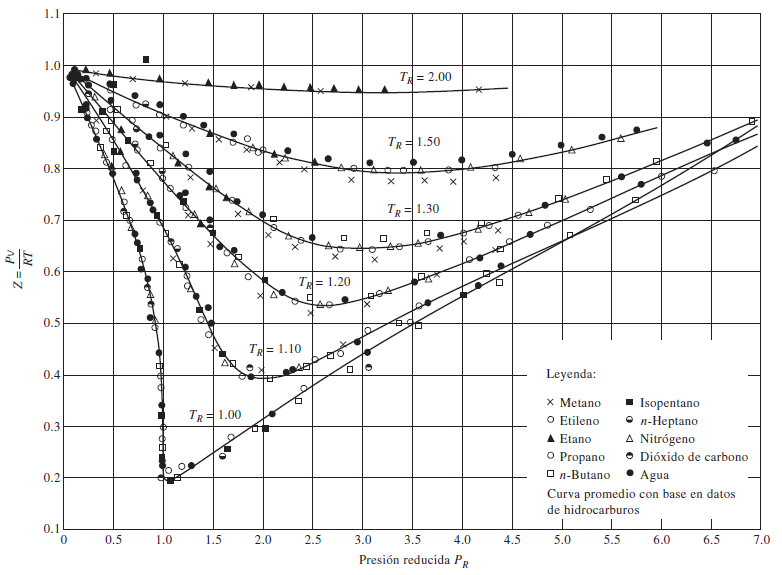
\includegraphics[width=\textwidth]{img/diagramas/par_red.png}
                \caption[Factor de Compresibilidad por presión reducida]{Factor de Compresibilidad por presión reducida \cite{cengel_termodinamica_2012}}
                \label{fig:par_red}
            \end{figure}
            
            \subsubsubsection{Diagrama de Nelson-Obert}
            
            \begin{figure}
                \centering
                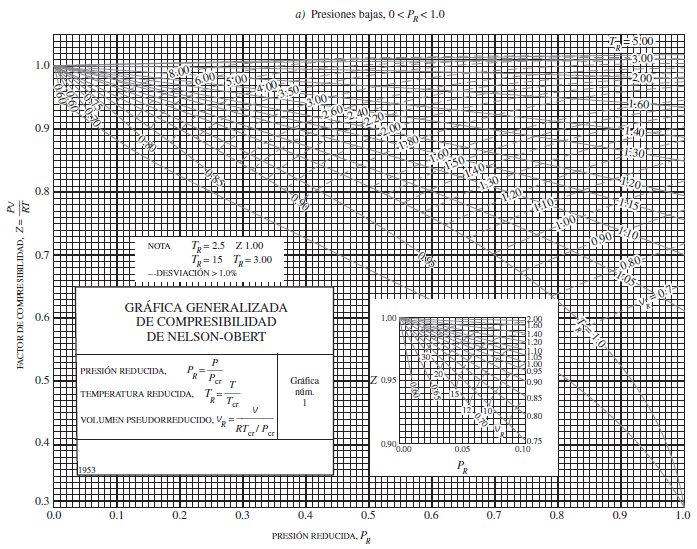
\includegraphics[width=\textwidth]{img/diagramas/nelson_obert_1.png}
                \caption[Gráfica Generalizada de Compresibilidad de Nelson-Obert (Presiones Bajas)]{Gráfica Generalizada de Compresibilidad de Nelson-Obert (Presiones Bajas) \cite{cengel_termodinamica_2012}}
                \label{fig:nelson_obert_1}
            \end{figure}
            
            \begin{figure}
                \centering
                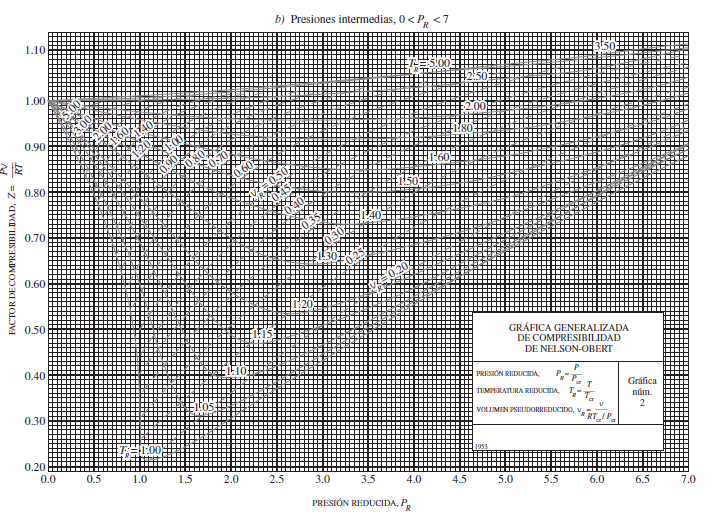
\includegraphics[width=\textwidth]{img/diagramas/nelson_obert_2.png}
                \caption[Gráfica Generalizada de Compresibilidad de Nelson-Obert (Presiones Intermedias)]{Gráfica Generalizada de Compresibilidad de Nelson-Obert (Presiones Intermedias) \cite{cengel_termodinamica_2012}}
                \label{fig:nelson_obert_2}
            \end{figure}
            
            \subsubsubsection{Ecuaciones de Estado Corregidas por no idealidades}
            
            \textbf{Ecuación de Van der Waals}:
            
            \begin{equation}
            \label{van_der_waals}
                \left ( P + \frac{a}{v^{2}}\right )\cdot (v-b) = RT
            \end{equation}
            
            \begin{equation}
                a=\frac{27R^{2}{T_{c}}^{2}}{64P_{c}}\wedge b=\frac{RT_{c}}{8P_{c}}
            \end{equation}
            
            \textbf{Peng-Robinson}:
            
            \begin{equation}
                P=\frac{RT}{v-b} - \frac{a\alpha}{v^{2}+2bv-b^{2}}
            \end{equation}
            \[a=0.42478\frac{R^{2}{T_{c}}^{2}}{P_{c}}\wedge b=0.08664\frac{RT_{c}}{P_{c}}\]
            \[\alpha = \left ( 1 + \kappa \left ( 1 - {T_{r}}^{\frac{1}{2}}\right ) \right )^{2} \wedge \kappa = 0.37464 + 1.54226\omega - 0.26992 {\omega}^{2} \wedge \omega = \text{factor acéntrico}\]
            
            \textbf{Soave-Redlich-Kwong}:
        
            \begin{equation}
                P=\frac{RT}{v-b} - \frac{a \lambda}{v(v+b)}
            \end{equation}
            \[a=0.42748\frac{R^{2}{T_{c}}^{2}}{P_{c}} \wedge b=0.08664\frac{RT_{c}}{P_{c}}\]
            \[\lambda=\left ( 1 + \kappa \left ( 1-{T_{r}}^{\frac{1}{2}} \right ) \right )^{2} \wedge \kappa=0.48+1.574\omega - 0.176 \omega^{2} \wedge \omega = \text{factor acéntrico}\]
            
            \textbf{Redlich-Kwong}:
        
            \begin{equation}
                P=\frac{RT}{v-b} - \frac{a}{\sqrt{T}v(v+b)}
            \end{equation}
            \[a=0.42748\frac{R^{2}{T_{c}}^{2.5}}{P_{c}} \wedge b=0.08664\frac{RT_{c}}{P_{c}}\]
            
            \subsubsubsection{Ecuaciones de Estado / Datos Experimentales}
            
            \begin{figure}
                \centering
                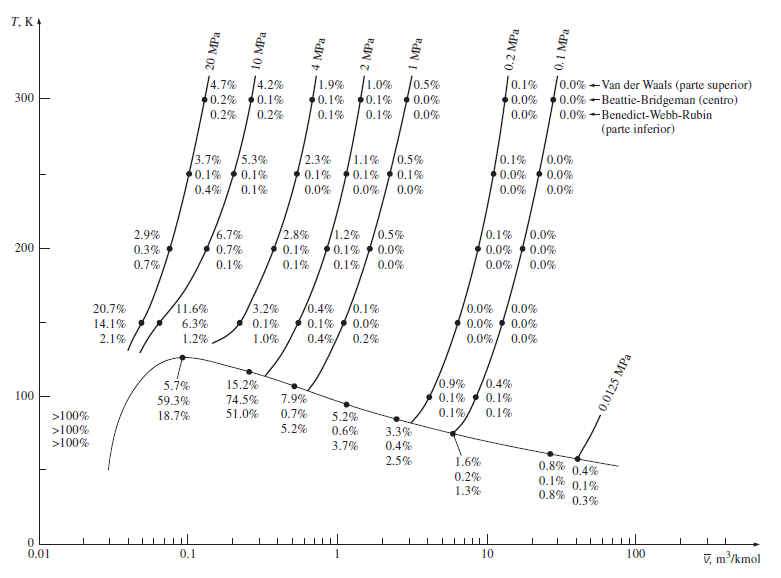
\includegraphics[width=.9\textwidth]{img/diagramas/error_estado.png}
                \caption[Porcentaje de error relacionado con las distintas ecuaciones de estado para el nitrógeno]{Porcentaje de error relacionado con las distintas ecuaciones de estado para el nitrógeno \cite{cengel_termodinamica_2012}}
                \label{fig:error_estado}
            \end{figure}
        
        \subsubsection{Mezcla de Gases Reales}
        
        \textbf{Método de Kay}
        
        \begin{quote}
            \textit{\say{Uso de valores pseudocríticos para mezclas de gases.}}
        \end{quote}
        
        \begin{equation}
        \label{eq:metodo_kay_p}
            {{P}^{'}}_{C} = P_{C, 1}y_{1} + P_{C, 2}y_{2} + \cdots = \sum_{i} P_{C, i}y_{i}
        \end{equation}
        \begin{equation}
        \label{eq:metodo_kay_t}
            {{T}^{'}}_{C} = T_{C, 1}y_{1} + T_{C, 2}y_{2} + \cdots = \sum_{i} T_{C, i}y_{i}
        \end{equation}
        \[{{P}^{'}}_{r} = \frac{P}{{{P}^{'}}_{C}} \wedge {{T}^{'}}_{r} = \frac{T}{{{T}^{'}}_{C}}\]
        
        \subsubsection{Mezclas Líquidas}
        
        \begin{equation}
        \label{eq:mezclas_liq}
            \frac{1}{\overline{\rho}} = \sum_{i=1}^{n} \frac{x_{i}}{\rho_{i}}
        \end{equation}
        
        Con \(\overline{\rho}\) la densidad promedio de la mezcla, \(\rho_{i}\) densidad del componente \(i\), \(x_{i}\) fracción molar del componente \(i\) y \(n\) el número de componentes.
    
    \subsection{Balances en sistema de Varias Fases}
        
        \subsubsection{Definiciones}
        
            \subsubsubsection{Punto Crítico}
            
            \begin{quote}
                \textit{\say{Temperatura y presión en la cual las propiedades de la fase líquida y gaseosa de una sustancia pura son idénticas.}}
            \end{quote}
            
            \subsubsubsection{Vapor}
            
            \begin{quote}
                \textit{\say{Gas por debajo de su punto crítico, se puede condensar.}}
            \end{quote}
            
            \subsubsubsection{Gas}
            
            \begin{quote}
                \textit{\say{No condensable, por encima de su punto crítico.}}
            \end{quote}
            
            \subsubsubsection{Vapor/líquido saturado}
            
            \begin{quote}
                \textit{\say{Cuando vapor y líquido se encuentran en equilibrio.}}
            \end{quote}
        
        \subsubsection{Separación}
        
            \subsubsubsection{Técnicas de separación}
            
            \begin{itemize}
                \item \textbf{Mecánica}: filtración, sedimentación, centrifugación.
                \item \textbf{Velocidad}: cromatografía.
                \item \textbf{Equilibrio}: destilación, cristalización
            \end{itemize}
            
            \subsubsubsection{Selección de metodología}
            
            Es mas difícil separar dos componentes en una fase que separar 2 fases (gas|líquido, sólido|líquido). La idea para un proceso de separación por equilibrio es llevar los componentes a fases distintas:
            
            \begin{itemize}
                \begin{minipage}{0.3\linewidth}
                    \item Destilación
                \end{minipage}
                \begin{minipage}{0.3\linewidth}
                    \item Cristalización
                \end{minipage}
                \begin{minipage}{0.3\linewidth}
                    \item Extracción con solventes
                \end{minipage}
            \end{itemize}
            
            \textbf{Separación por equilibrio}
            
            Se alimenta una mezcla multicomponente en una fase. En el separador se genera una segunda fase. Las composiciones de las fases son diferentes. Dependen de la termodinámica. Ambas fases tienen igual \(P\), \(T\).
        
            \subsubsubsection{Reglas de las fases de Gibbs}
            
            Se aplica solo a sistemas en equilibrio. Dos fases en contacto, sus componentes se redistribuyen hasta el equilibrio.
            
            Número de grados de libertad (\textbf{variables intensivas}) de un sistema de varias fases (\(P\), \(T\), \(\rho\), \(x_{i}\), \(y_{i}\)):
            
            \begin{equation}
            \label{eq:reglas_fases_gibbs}
                F = 2 + m - \pi
            \end{equation}
            
            Con \(m\) número de sustancias químicas (si no existe reacción química) y \(\pi\) número de fases.
            
            \subsubsubsection{Medidas de desempeño}
            
            \textbf{Pureza fraccionaria}:
            
            \begin{quote}
                \textit{\say{Cantidad de moles del componente deseado en un cierto producto por la cantidad de moles de dicho producto.}}
            \end{quote}
            
            \begin{equation}
            \label{eq:pureza_fraccionaria}
                x_{ij} = \frac{\text{moles componente deseado }i\text{ en producto} j}{\text{moles de corriente de producto }j} = \frac{\dot{n}_{ij}}{\dot{n}_{j}}
            \end{equation}
            \newpage
            
            \textbf{Recuperación fraccionaria}:

            \begin{quote}
                \textit{\say{Cantidad de moles del componente deseado en un cierto producto por la cantidad de moles de cierto componente en la alimentación.}}
            \end{quote}
            
            \begin{equation}
            \label{eq:recuperacion_fraccionaria}
                f_{Rik} = \frac{\text{moles componente deseado }i\text{ en producto} j}{\text{moles componente }k\text{ en la Alimentación}} = \frac{\dot{n}_{ij}}{\dot{n}_{kA}}
            \end{equation}
            
            \textbf{Factor de Separación}:
            
            \begin{equation}
            \label{eq:factor_separacion}
                \alpha_{BC} = \frac{\text{moles }B\text{ en }1}{\text{moles }C\text{ en }1} \frac{\text{moles }C\text{ en }2}{\text{moles }B\text{ en }2} = \frac{\dot{n}_{B1}}{\dot{n}_{C1}} \frac{\dot{n}_{C2}}{\dot{n}_{B2}}
            \end{equation}
        
        \subsubsection{Diagrama de Fases del Agua}
        
            \subsubsubsection{Presión de Vapor}
            
            \begin{quote}
                \textit{\say{Presión de equilibrio en la que el vapor y el líquido de un componente puro están en equilibrio.}}
            \end{quote}
            
            \textbf{Estimaciones}:
            
            \textbf{Clausius-Clapeyron}:
            
            \[\frac{dP^{*}}{dT} = \frac{\Delta \widehat{H}_{V}}{T \left ( \widehat{V}_{g} - \widehat{V}_{l} \right )}\]
            
            Con \(\Delta \widehat{H}_{V}\) calor (o entalpía) de vaporización.
            
            Asumiendo que el volumen del gas es mucho mayor que la del líquido y que se trata de un gas ideal:
            
            \[\overset{\widehat{V}_{g} >> \widehat{V}_{l}}{\Rightarrow} \frac{dP^{*}}{dT} = \frac{\Delta \widehat{H}_{V}}{T \left ( \widehat{V}_{g} \right )} \overset{\text{Gas ideal}}{=} \frac{\Delta \widehat{H}_{V} P^{*}}{RT^{2}}\]
            
            \[\Rightarrow \frac{dP^{*}}{P^{*}} = \frac{\Delta \widehat{H}_{V}}{RT^{2}}dT \overset{\int{}}{\Rightarrow} \overset{\Delta \widehat{H}_{V}\text{ constante en un amplio rango de }T}{\Rightarrow}\]
            
            \begin{equation}
            \label{eq:clausius_clapeyron}
                \ln{P^{*}} = -\frac{\Delta \overline{H}_{V}}{RT} + B
            \end{equation}
            
            \begin{equation}
            \label{eq:clausius_clapeyron_interval}
                \ln{\frac{P_{2}^{*}}{P_{1}^{*}}} = -\frac{\Delta \overline{H}_{V}}{R} \left ( \frac{1}{T_{2}} - \frac{1}{T_{1}} \right )
            \end{equation}
            
            \textbf{Ecuación de Antoine}:
            \begin{equation}
            \label{eq:antoine}
                \ln{P^{*}} = A - \frac{B}{C+T}
            \end{equation}
            
            Con \(A,B,C\) constantes.
            
            Diagrama de Cox (\textbf{Figura \ref{fig:diag_cox}}).
            
            \begin{figure}
                \centering
                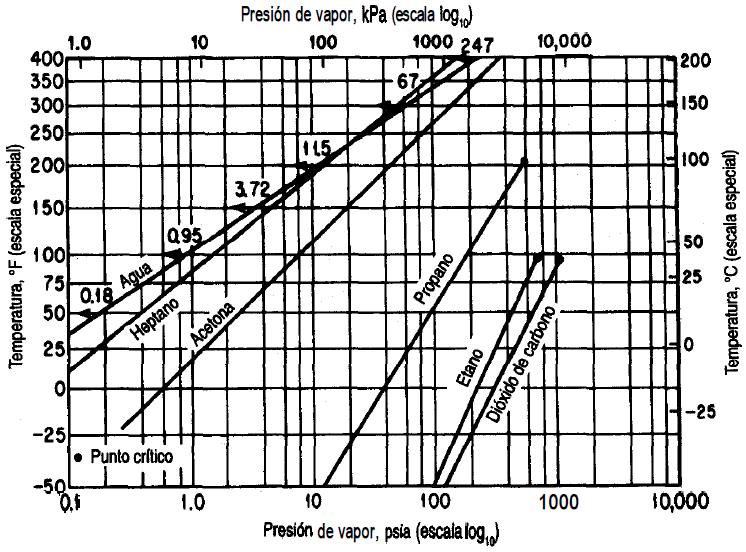
\includegraphics[width=.7\textwidth]{img/diagramas/diagrama_cox.png}
                \caption[Diagrama de Cox]{Diagrama de Cox \cite{himmelblau_principios_1997}}
                \label{fig:diag_cox}
            \end{figure}
            
    \subsection{Equilibrio para sistemas multicomponentes}
    
    Involucra \(P\), \(T\) y fracciones de cada componente en las fases.
    
        \subsubsection{Sistema Vapor-Gas}
        
            \subsubsubsection{Saturación}
            
            \begin{quote}
                \textit{\say{Un gas en equilibrio con un líquido, debe estar saturado con ese líquido. Si un gas a temperatura \(T\) y presión \(P\) contiene un vapor saturado cuya fracción molar es \(y_{v}\) y si este vapor es la única sustancia condensable, entonces la \textbf{presión parcial} de vapor en el gas es igual a la \textbf{presión de vapor del componente puro} a la temperatura del sistema.}}
            \end{quote}
            
            \begin{equation}
            \label{eq:sat}
                P_{V} = y_{V} \cdot P = P_{V}^{*}(T)
            \end{equation}
            
            \subsubsubsection{Condiciones de Saturación}
            
            \begin{itemize}
                \item \(P_{V} = P_{V}^{*}(T)\): El vapor está \textbf{saturado}. Si se añade más vapor a la fase gas o se aumenta la presión total, se producirá condensación.
                \item \(P_{V} = y_{V}\cdot P < P_{V}^{*}(T)\): El vapor está \textbf{sobrecalentado}.
            \end{itemize}
        
            \subsubsubsection{Punto de Rocío}
            
            \begin{quote}
                \textit{\say{Temperatura a la que se satura el único vapor sobrecalentado presente en un gas, al enfriarse a presión constante.}}
            \end{quote}
            
            En saturación se cumple la \textbf{Ecuación \ref{eq:punto_rocio}}, con \(T_{PR}\) punto de rocío.
            
            \begin{equation}
            \label{eq:punto_rocio}
                P_{V} = y_{V}\cdot P = P_{V}^{*}\left ( T_{PR} \right )
            \end{equation}
        
            \subsubsubsection{Grado de Sobrecalentamiento}
            
            \begin{quote}
                \textit{\say{Diferencia entre la temperatura de un gas y su punto de rocío.}}
            \end{quote}
        
        \subsubsection{Sistema Líquido-Vapor}
        
            \subsubsubsection{Diagramas Líquido-Vapor}
            
            \begin{quote}
                \textit{\say{Muestran las composiciones de equilibrio de un sistema, como función de \(T\).}}
            \end{quote}
            
            \begin{figure}
                \centering
                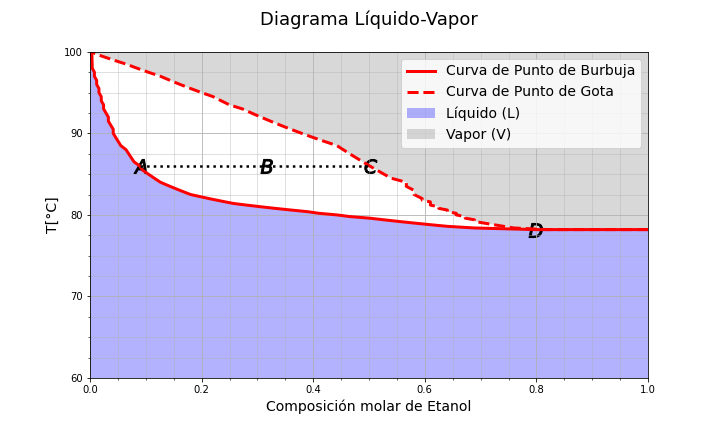
\includegraphics[width=.7\textwidth]{img/graficos/diag_l_v_etanol.png}
                \caption{Diagrama Líquido-Vapor del Etanol}
                \label{fig:diag_l_v_etanol}
            \end{figure}
            
            En la \textbf{Figura \ref{fig:diag_l_v_etanol}} el punto \(\mathbf{D}\) representa el \textbf{punto Azeótropo}. A cierta temperatura \(T\) (marcada por los puntos \(\mathbf{A, B, C}\)) se tiene que:
            \[f_{V} = \frac{n_{V}}{\left ( n_{V} + n_{L}\right )} = \frac{\overline{AB}}{\overline{AC}} \wedge f_{L} = \frac{n_{L}}{\left ( n_{V} + n_{L}\right )} = \frac{\overline{BC}}{\overline{AC}} \Rightarrow \frac{\frac{n_{V}}{\cancel{\left ( n_{V} + n_{L}\right )}}}{\frac{n_{L}}{\cancel{\left ( n_{V} + n_{L}\right )}}} = \frac{\frac{\overline{AB}}{\cancel{\overline{AC}}}}{\frac{\overline{BC}}{\cancel{\overline{AC}}}} \Rightarrow\]
            \[\frac{n_{V}}{n_{L}} = \frac{\overline{AB}}{\overline{BC}}\]
            \newpage
        
            \subsubsubsection{Ley de Henry}
            
            \begin{quote}
                \textit{\say{Válida para fracción molar cercana a cero.}}
            \end{quote}
            
            \begin{equation}
            \label{eq:ley_henry}
                P_{i} = y_{i} \cdot P_{T} = H_{i}(T) \cdot x_{i}
            \end{equation}
            
            Con \(H_{i}(T)\) constante de Henry.
        
            \subsubsubsection{Ley de Raoult}
        
            \begin{quote}
                \textit{\say{Válida para fracción molar cercana a uno (casi puro en fase líquida) o mezclas de sustancias similares.}}
            \end{quote}
            
            \[P_{i} = P_{i}^{*}(T) \cdot x_{i}\]
            
            Ley de Dalton:
            \[P_{i} = y_{i} \cdot P_{T} \overset{\text{Ley de Raoult}}{\Rightarrow}\]
            
            \begin{equation}
            \label{eq:ley_raoult}
                P_{i} = y_{i} \cdot P_{T} = P_{i}^{*}(T) \cdot x_{i}
            \end{equation}
            
            Constante de equilibrio \(K_{i}\):
            \[K_{i} = \frac{y_{i}}{x_{i}} = \frac{P_{i}^{*}}{P_{T}}\]
            \begin{quote}
                \textit{\say{En un sistema de multicomponente de dos fases, un componente en una fase está en equilibrio con el mismo componente en la otra fase.}}
            \end{quote}
        
            \subsubsubsection{Punto de Burbuja}
            
            \begin{quote}
                \textit{\say{Se calienta una mezcla líquida a \(P\) constante hasta que se forma una \textbf{burbuja} de vapor.}}
            \end{quote}
            \[P_{i} = x_{i} \cdot P_{i}^{*} \left ( T_{PB} \right )\]
            \[P_{T} = \sum_{i} P_{i} \overset{\text{Punto de burbuja}}{=} \sum_{i} \left ( x_{i} \cdot P_{i}^{*} \left ( T_{PB} \right ) \right )\]
            \begin{equation}
            \label{eq:punto_burbuja}
                y_{i} = \frac{P_{i}}{P_{T}} = \frac{x_{i} \cdot P_{i}^{*}}{P_{T}}
            \end{equation}
            
            Con \(P_{i}^{*}\) obtenidos de tablas o correlaciones.
        
            \subsubsubsection{Punto de Rocío}
            
            \begin{quote}
                \textit{\say{Se enfría una mezcla a \(P\) constante hasta que se forma una \textbf{gota} de líquido en equilibrio con el vapor.}}
            \end{quote}
            
            Reescribiendo la \textbf{Ecuación \ref{eq:punto_rocio}}:
            \[P_{i} = y_{i}\cdot P_{T} = x_{i} \cdot P_{i}^{*}\left ( T_{PR} \right ) \Rightarrow x_{i} = \frac{y_{i}\cdot P_{T}}{P_{i}^{*}\left ( T_{PR} \right )}\]
            
            Como:
            \[\sum_{i}x_{i} = 1 \Rightarrow\]
            
            \begin{equation}
            \label{eq:punto_rocio_2}
                \sum_{i} \left ( \frac{y_{i}\cdot P_{T}}{P_{i}^{*}\left ( T_{PR} \right )} \right ) = 1
            \end{equation}
            
            Con \(P_{i}^{*}\) obtenidos de tablas o correlaciones.
        
        \subsubsection{Sistema Líquido-Vapor: Saturación Parcial}
        
            \subsubsubsection{Sistema Aire-Vapor de agua}
            
            Se define:
            
            \begin{itemize}
                \item \(P_{i}\): Presión parcial del vapor en la mezcla.
                \item \(P_{i}^{*}\): Presión parcial del vapor en la mezcla si el gas se encuentra saturado a la temperatura de la mezcla (Presión de vapor).
            \end{itemize}
            
            \textbf{Humedad/Saturación Relativa}:
            
            \begin{equation}
            \label{eq:humedad_relativa}
                S_{r} = \frac{P_{i}}{P_{i}^{*}}
            \end{equation}
            
            \textbf{Humedad/Saturación Absoluta}:
            
            \begin{equation}
            \label{eq:humedad_absoluta}
                S_{a} = \frac{m_{\text{vapor}}}{m_{\text{gas seco}}}
            \end{equation}
            
            \textbf{Humedad/Saturación molal}:
            
            \begin{equation}
            \label{eq:humedad_molal}
                S_{m} = \frac{P_{i}}{P_{T} - P_{i}} = \frac{\text{moles vapor}}{\text{moles gas libres de vapor (gas seco)}}
            \end{equation}
            
            \textbf{\% Humedad/ \%Saturación (molal)}:
            
            \begin{equation}
            \label{eq:per_humedad_molal}
                S_{p} = \frac{S_{m}}{S_{m}^{*}} \cdot 100
            \end{equation}
        \newpage
            
        \subsubsection{Sistema Sólido-Líquido}
        
            \subsubsubsection{Saturación Sólido-Líquido}
            
            \begin{quote}
                \textit{``Existe un límite en la cantidad de soluto que se puede disolver en un solvente. Depende de la temperatura.}
                
                \textit{``Una disolución que contiene tanta cantidad de una sustancia como es capaz de disolver se llama saturada.}
                
                \textit{``Si se enfría una solución saturada, la solubilidad del soluto disminuye, precipita y se forman cristales. Por lo tanto, una solución en equilibrio con cristales de un soluto, debe estar saturada con ese soluto.''}
            \end{quote}
            
            \subsubsubsection{Solubilidad de diferentes solutos en el agua}
            
            \begin{figure}
                \centering
                \includegraphics[width=.6\textwidth]{img/graficos/solubilidad_solutos.png}
                \caption{Solubilidad de diferentes solutos en agua a diferentes temperaturas}
                \label{fig:solubilidad_agua}
            \end{figure}
        
            \subsubsubsection{Diagrama Sólido-Líquido}
            
            \begin{quote}
                \textit{\say{Muestran composiciones de equilibrio de un sistema, como función de una o más variables de éste.}}
            \end{quote}
            
            \begin{figure}
                \centering
                \includegraphics[width=.95\textwidth]{img/diagramas/diagrama-s-l.png}
                \caption[Ejemplo diagrama Sólido Líquido para el \(MgS{O}_{4}\) en \(H_{2}O\)]{Ejemplo diagrama Sólido Líquido para el \(MgS{O}_{4}\) en \(H_{2}O\) \cite{perry_perrys_1963}}
                \label{fig:diag_s-l}
            \end{figure}
            
            \subsubsubsection{Regla de la Palanca}
            
            \begin{quote}
                \textit{\say{Se usa para determinar la fracción (másica/molar) de cada una de las fases de un equilibrio binario desde un diagrama de fases.}}
                
                \textit{\say{Si se tienen dos fases \(\alpha\), \(\beta\) en las que cada una contiene dos elementos \(A\) y \(B\), la fracción de la fase \(\alpha\) es:}}
            \end{quote}
            
            \begin{equation}
            \label{eq:regla_palanca}
                x_{\alpha} = \frac{x_{B} - x_{(B, \beta)}}{x_{(B, \alpha)} - x_{(B, \beta)}}
            \end{equation}
            
            Usando la \textbf{Figura \ref{fig:diag_s-l}} se puede obtener las composiciones en dos fases desde la composición total de una especie (en este caso \(MgS{O}_{4}\)). Para ello se siguen los siguientes pasos:
            
            \begin{enumerate}
                \item Se ubica la fracción total de la especie en el eje de la fracción (abscisa).
                \item Se identifica con la temperatura a la que se encuentra la mezcla (ordenada).
                \item El punto encontrado se extiende (horizontalmente) hasta la líneas de equilibrio (líneas diagonales y verticales dentro del gráfico). Cada línea representa una fase.
                \item Desde los puntos de intersección de cada línea de equilibrio, se busca la fracción de la especie para cada fase (abscisa).
            \end{enumerate}
            
            \subsubsubsection{Propiedades coligativas}
            
            \textbf{Disminución de la presión de vapor}:
            
            \[P_{d} = \left ( 1 - x \right ) P_{d}^{*}\]
            
            Con \(P_{d}^{*}\) presión de vapor del disolvente puro y \(x\) la fracción mola de soluto.
            
            Se define \(\left ( P_{d}^{*} \right )_{e}\) la presión de vapor efectiva del disolvente en presencia de un soluto \textbf{no volátil, no disociable}. Ésta es igual a la presión parcial del disolvente en fase vapor (\(P_{d}\)) en equilibrio con la disolución:
            
            \[\left ( P_{d}^{*} \right )_{e} = P_{d} = \left ( 1 - x \right ) P_{d}^{*}\]
            \[\text{Con }\Delta P_{d}^{*} = P_{d}^{*} - \left ( P_{d}^{*} \right )_{e} \Rightarrow \Delta P_{d}^{*} = P_{d}^{*} - \left ( 1 - x \right ) P_{d}^{*} \Rightarrow\]
            \begin{equation}
            \label{eq:dis_presion_vapor}
                \Delta P_{d}^{*} = x P_{d}^{*}
            \end{equation}
            
            El efecto de la disminución de la presión de vapor del disolvente debido a la presencia del soluto (no volátil) (\textbf{Ecuación \ref{eq:dis_presion_vapor}}) es que a una determinada presión éste hierve a una temperatura mayor y se congela a una temperatura menor que el disolvente puro a la misma presión.
        
            \textbf{Aumento en el punto de ebullición}:
            
            \begin{equation}
            \label{eq:aum_punto_ebull}
                \Delta T_{e} = T_{se} - T_{0e} = \frac{R{T_{0e}}^{2}}{\Delta \widehat{H}_{V}} x
            \end{equation}
            
            \textbf{Disminución en el punto de congelación}:
            
            \begin{equation}
            \label{eq:dis_punto_cri}
                \Delta T_{f} = T_{0f} - T_{sf} = \frac{R{T_{0f}}^{2}}{\Delta \widehat{H}_{F}} x
            \end{equation}
            
        \subsubsection{Sistema Líquido-Líquido}
        
            \subsubsubsection{Líquidos inmiscibles y parcialmente miscibles}
            
            \textbf{Líquidos Miscibles}:
            
            \begin{quote}
                \textit{\say{Si al mezclarse en cualquier proporción forman una solución homogénea (1 fase).}}
            \end{quote}
            
            \textbf{Líquidos Parcialmente Miscibles}:
            
            \begin{quote}
                \textit{\say{Si dos líquidos forman una fase bajo ciertas condiciones y dos fases en otras condiciones.}}
            \end{quote}
            
            \textbf{Líquidos Inmiscibles}:
            
            \begin{quote}
                \textit{\say{Cuando dos sustancias no tienen la capacidad de constituir una solución homogénea.}}
            \end{quote}
            
            \textbf{Coeficiente de Distribución}:
            
            Al añadir una tercera sustancia a una mezcla de dos fases líquidas, se distribuye de acuerdo con su solubilidad relativa en cada fase (extracción en fase líquida).
            
            \begin{quote}
                \textit{\say{Sean \(A\) y \(S\) dos líquidos \textbf{casi inmiscibles} y \(B\) un soluto, el coeficiente de distribución (o partición) de \(B\) se define como la razón entre la fracción de \(B\) en \(S\) y la fracción de \(B\) en \(A\).}}
            \end{quote}
            
            \begin{equation}
            \label{eq:coef_distribucion}
                K = \frac{x_{B}^{S}}{x_{B}^{A}}
            \end{equation}
            
            \subsubsubsection{Sistemas Ternarios}
            
            Para sistemas de tres componentes, parcialmente miscibles, su comportamiento se presenta en un diagrama de fases triangular, donde cada vértice representa un componente, y los lados representan soluciones binarias. Las líneas de unión indican las composiciones de las fases en equilibrio.
            
            \begin{figure}
                \centering
                \includegraphics[width=\textwidth]{img/diagramas/sistema_ternario.png}
                \caption{Sistema ternario Metil isobutil cetona-Acetona-Agua}
                \label{fig:sistema_ternario}
            \end{figure}
        
    \subsection{Procesos Intermitentes}
    
    El proceso ocurre en un período de tiempo entre \(t_{0}\) y \(t_{f}\). Considera cantidades iniciales y finales de masa en el sistema. Recordando \textbf{Ecuación \ref{eq:balance_masa}}:
    \[\text{Flujo entrada} - \text{Flujo salida} + \text{Generación} - \text{Consumo} = \text{Acumulación}\]
    
        \subsubsection{Sin reacción}
        \[\text{Acumulación} = \text{Flujo entrada} - \text{Flujo salida} + \cancelto{0}{\text{Generación}} - \cancelto{0}{\text{Consumo}}\]
        
        \textbf{Masa Total}:
        
        \begin{itemize}
            \item Forma diferencial:
            \begin{equation}
            \label{eq:proc_int_sin_tot_dif}
                \frac{dm_{sis}}{dt} = \sum_{\text{entrada}}\dot{m}_{j} - \sum_{\text{salida}}\dot{m}_{j}
            \end{equation}
            \item Forma integral:
            \begin{equation}
            \label{eq:proc_int_sin_tot_int}
                m_{sis, f} - m_{sis, 0} = \sum_{\text{entrada}}\left ( \int_{t_{0}}^{t_{f}}\dot{m}_{j}dt \right ) - \sum_{\text{salida}}\left ( \int_{t_{0}}^{t_{f}}\dot{m}_{j}dt \right )
            \end{equation}
        \end{itemize}
        
        \textbf{Masa de un componente \(i\)}:
        
        \begin{itemize}
            \item Forma diferencial:
            \begin{equation}
            \label{eq:proc_int_sin_i_dif}
                \frac{dm_{i, sis}}{dt} = \sum_{\text{entrada}}\dot{m}_{ij} - \sum_{\text{salida}}\dot{m}_{ij}
            \end{equation}
            \item Forma integral:
            \begin{equation}
            \label{eq:proc_int_sin_i_int}
                m_{i, sis, f} - m_{i, sis, 0} = \sum_{\text{entrada}}\left ( \int_{t_{0}}^{t_{f}}\dot{m}_{ij}dt \right ) - \sum_{\text{salida}}\left ( \int_{t_{0}}^{t_{f}}\dot{m}_{ij}dt \right )
            \end{equation}
        \end{itemize}
    
        Con \(i\) componentes y \(j\) corrientes.
        
        \subsubsection{Con reacción}
        \[\text{Acumulación} = \text{Flujo entrada} - \text{Flujo salida} + \text{Generación} - \text{Consumo}\]
        
        \textbf{Masa de un componente \(i\)}:
        
        \begin{itemize}
            \item Forma diferencial:
            \begin{equation}
            \label{eq:proc_int_con_i_dif}
                \frac{dm_{i, sis}}{dt} = \sum_{\text{entrada}}\dot{m}_{ij} - \sum_{\text{salida}}\dot{m}_{ij} + \sum_{\text{reacción}}\dot{R}_{ik}
            \end{equation}
            \item Forma integral:
            \begin{equation}
            \label{eq:proc_int_con_i_int}
                m_{i, sis, f} - m_{i, sis, 0} = \sum_{\text{entrada}}\left ( \int_{t_{0}}^{t_{f}}\dot{m}_{ij}dt \right ) - \sum_{\text{salida}}\left ( \int_{t_{0}}^{t_{f}}\dot{m}_{ij}dt \right ) + \sum_{\text{reacción}}\left ( \int_{t_{0}}^{t_{f}}\dot{R}_{ik}dt \right )
            \end{equation}
        \end{itemize}
        
        Con \(k\) reacciones.
    
\newpage
            
\section{Balances de Energía en Estado Estacionario}
    
\begin{quote}
    \say{\textit{El ingeniero de diseño de procesos deberá \textbf{cuantificar la energía} que entra o sale de cada operación unitaria y determinar las necesidades globales de energía para el proceso. \textbf{Los costos asociados} a los requerimientos energéticos de los procesos deben ser considerados en el costo total de los procesos.}}
\end{quote}

Los \textbf{balances de energía} permiten determinar los requerimientos energéticos de un proceso y posibles vías de ahorro de energía.

La energía puede adoptar diferentes formas, todas ellas convertibles directa o indirectamente de una en otra.

Análogamente a lo establecido para el Balance de Masa, se definen los límites del sistema y consideramos lo que cruza dichos límites.

\begin{figure}
    \centering
    \includegraphics[width=.8\textwidth]{img/diagramas/balance_energia.png}
    \caption[Conversión de Energía]{Conversión de Energía \cite{martinez_salas_transformacion_2013}}
    \label{fig:balance_energia}
\end{figure}

\begin{equation}
\label{eq:balance_energia}
    E_{\text{acumulada}} = E_{\text{entra}} - E_{\text{sale}} + E_{\text{producida}} - E_{\text{consumida}}
\end{equation}

    \subsection{Formas de Energía}
    
    Principales formas de energía a considerar en una corriente.
    
        \subsubsection{Energía Potencial}
        
        Debida a la posición en un campo potencial (campo gravitacional o magnético).
        
        \begin{equation}
        \label{eq:e_potencial}
            E_{P} = mgh
        \end{equation}
        
        Con \(m\) masa, \(g\) acelaración de gravedad y \(h\) altura.
        
        \subsubsection{Energía Cinética}
        
        Debida al movimiento del sistema como un todo respecto a algún marco de referencia.
        
        \begin{equation}
        \label{eq:e_cinetica}
            E_{K} = \frac{mv^{2}}{2}
        \end{equation}
        
        Con \(v\) velocidad.
        
        \subsubsection{Energía Interna}
        
        Debida al movimiento de las moléculas con respecto al centro de masa del sistema, al movimiento de rotación y de vibración, a las interacciones electromagnéticas de las moléculas y al movimiento y las interacciones de los constituyentes atómicos o subatómicos de las moléculas.
        
        \begin{equation}
        \label{eq:e_interna}
            \widehat{U} \cong f(T)
        \end{equation}
        
        Con \(T\) temperatura y \(f\) una función de \(T\).
        
        \subsubsection{Función de Estado}
        
        No depende de la trayectoria.
        
    \subsection{Transferencia de Energía}
    
    Un sistema no contiene calor, \textbf{pero la transferencia de calor o trabajo} hacia o desde el sistema, altera su contenido de \textbf{energía interna}.
    
        \subsubsection{Trabajo \(W\)}
        
        Transferencia de energía debido a la acción de una fuerza mecánica que vence una resistencia al recorrer una distancia.
        
        \textbf{Convención}:
        
        \begin{itemize}
            \item \(W > 0\) (positivo) si el sistema \textbf{realiza} trabajo.
            \item \(W < 0\) (negativo) si se realiza trabajo \textbf{sobre} el sistema.
        \end{itemize}
        
        \textbf{Formas de energía en \(W\)}:
        
        \begin{itemize}
            \item \textbf{Energía Mecánica}: En los procesos se debe a la agitación, vibración, bombeo, soplado, compresión, etc.
            \item \textbf{Energía Eléctrica}: En los equipos eléctricos y electrónicos asociados a los equipos de proceso. Es muy importante en los procesos electroquímicos: pilas, baterías, electro obtención, electro refinación, electrodiálisis, etc.
        \end{itemize}
        
        \subsubsection{Calor \(Q\)}
        
        Transferencia de energía ocasionada por una diferencia de temperaturas.
        
        \textbf{Convención}:
        
        \begin{itemize}
            \item \(Q > 0\) (positivo) si se \textbf{agrega} calor al sistema.
            \item \(Q < 0\) (negativo) si se \textbf{extrae} calor del sistema.
        \end{itemize}
        
        La temperatura representa la velocidad promedio del movimiento molecular en esa materia. Ejemplos de expresiones para la velocidad de transferencia de calor:
        
        \begin{itemize}
            \item Conducción:
                \begin{equation}
                \label{eq:calor_conduccion}
                    \dot{Q} = -kA \nabla T
                \end{equation}
            \item Convección:
                \begin{equation}
                \label{eq:calor_conveccion}
                    \dot{Q} = hA \left ( T_{\inf} - T_{w} \right )
                \end{equation}
            \item Radiación:
                \begin{equation}
                \label{eq:calor_radiacion}
                    \dot{Q} = \sigma \left ( {T_{\inf}}^{4} - {T_{w}}^{4} \right )
                \end{equation}
        \end{itemize}
        
        \subsubsection{Entalpía}
        
        La entalpía H es una función termodinámica definida en la \textbf{Ecuación \ref{eq:entalpia}}
        
        \begin{equation}
        \label{eq:entalpia}
            H = U + pV
        \end{equation}
        
        Se puede decir que la entalpía caracteriza la capacidad de un sistema para transferir calor hacia otro sistema. En un proceso a \underline{presión constante} tenemos:
        
        \[\overset{\text{\textbf{Ecuación \ref{eq:entalpia}}}}{\Rightarrow} dH = dU + d(pV) = dU + pdV + Vdp \overset{p = ctr}{=} dU + pdV\]
        
        Si no se produce otro trabajo que el de expansión:
        \begin{equation}
        \label{eq:trabajo_expansion}
            W = pdV
        \end{equation}
        
        Del primer principio de la termodinámica:
        \begin{equation}
        \label{eq:primer_principio}
            dU = Q - W
        \end{equation}
        
        Reemplazando la \textbf{Ecuación \ref{eq:trabajo_expansion}} en la \textbf{Ecuación \ref{eq:primer_principio}}:
        \[dU = Q - pdV \Leftrightarrow Q = dU + pdV\]
        
        Igualando la \textbf{Ecuación \ref{eq:entalpia}} en su forma diferencial y la ecuación anterior se obtiene:
        \begin{equation}
        \label{eq:h_q}
            dH = Q
        \end{equation}
        
        \begin{quote}
            \textit{\say{La variación de la entalpía es igual al calor absorbido.}}
        \end{quote}
        
        En sistemas sólidos o líquidos, la variación de \(pV\) es pequeña y:
        \begin{equation}
        \label{eq:sis_sol_liq_e_int}
            dU \cong dH
        \end{equation}
    
    \subsection{Balance de Energía sin Reacción Química}
    
        \subsubsection{Sistemas Cerrados}
        
        No intercambian masa, sólo energía.
        
        \begin{equation}
        \label{eq:energia_sis_cerrado}
            \Delta E = \Delta \left ( U + K + P \right ) = Q - W
        \end{equation}
        
        Estado estacionario:
        \begin{equation}
        \label{eq:energia_sis_cerrado_estacionario}
            \Delta E = 0 \rightarrow Q = W
        \end{equation}
        
        \subsubsection{Sistemas Abiertos}
        
        Intercambian masa y energía.
        
        En forma general:
        \begin{equation}
        \label{eq:energia_sis_abierto}
            \begin{matrix}
                 \Delta E & = & \Delta \left ( U + K + P \right ) & + & \Delta \left ( pV \right ) & + Q - W \\
                  & & \text{Energía transferida con la masa} & & \text{Trabajo de flujo} &
            \end{matrix}
        \end{equation}
        \[\Delta \widehat{H} = \Delta \widehat{U} + \Delta \left ( pV \right ) \Rightarrow\]
        \[\Delta E = m_{\text{entra}} \left ( \widehat{H} + \widehat{K} + \widehat{P} \right )_{\text{entra}} - m_{\text{sale}} \left ( \widehat{H} + \widehat{K} + \widehat{P} \right )_{\text{sale}} + Q - W\]
        
        Estado estacionario:
        \begin{equation}
        \label{eq:energia_sis_abierto_estacionario}
            \Delta E = 0 \rightarrow m_{\text{sale}} \left ( \widehat{H} + \widehat{K} + \widehat{P} \right )_{\text{sale}} - m_{\text{entra}} \left ( \widehat{H} + \widehat{K} + \widehat{P} \right )_{\text{entra}} = Q - W
        \end{equation}
    
    \subsection{Balance de Energía con y sin reacción química}
    
        \subsubsection{Capacidad calorífica y calor específico}
        
        Capacidad calorífica \(C\) es extensiva, calor específico \(\widehat{C}\) es intensiva y es por cantidad de materia (masa o mol):
        \[\widehat{C} = \frac{C}{m} \vee \widehat{C} = \frac{C}{n}\]
        
            \subsubsubsection{Capacidad calorífica a presión constante (\(C_{P}\))}
            
            \begin{quote}
                \textit{\say{Razón de incremento de la entalpía (\(H\)) por unidad de incremento de la temperatura a presión constante.}}
            \end{quote}
            
            \begin{equation}
            \label{eq:c_p}
                C_{P} = \left ( \frac{\partial H}{\partial T} \right )_{P}
            \end{equation}
            
            \subsubsubsection{Capacidad calorífica a volumen constante (\(C_{V}\))}
            
            \begin{quote}
                \textit{\say{Razón de incremento de la energía interna (\(U\)) por unidad de incremento de la temperatura a volumen constante.}}
            \end{quote}
            
            \begin{equation}
            \label{eq:c_v}
                C_{V} = \left ( \frac{\partial U}{\partial T} \right )_{V}
            \end{equation}
            
            \subsubsubsection{Propiedades}
            
            Líquidos y sólidos:
            \[C_{P} = C_{V}\]
            
            Gases Ideales:
            \[C_{P} = C_{V} + R\]
            
            Con \(R\) constante de los gases ideales.
            
            Tanto \(C_{P}\) como \(C_{V}\) son propiedades específicas de las sustancias y se encuentran tabulados.
            
            Tanto \(C_{P}\) como \(C_{V}\) son funciones de la temperatura y se expresan como polinomios cuyos parámetros se encuentran en tablas:
            \[C_{P} = A + BT + C{T}^{2} + D{T}^{3}\]
            
            \(C_{P}\) se puede calcular en forma gráfica \cite{perry_perrys_1963}.
            
            \subsubsubsection{\(C_{P}\) promedio}
            
            \begin{equation}
            \label{eq:cp_promedio}
                \overline{C_{P}} = \frac{1}{\left ( T - T_{Ref} \right )} \int_{T_{Ref}}^{T} C_{P} dT
            \end{equation}
            
            \subsubsubsection{\(C_{P}\) mezcla de gas ideal}
            
            \begin{equation}
            \label{eq:cp_mezcla}
                C_{P, \text{mezcla}} = \int_{i = 1}^{n} y_{i}C_{P, i}
            \end{equation}
        
        \subsubsection{Cálculo de entalpía}
        
            \subsubsubsection{Simplificaciones}
            
            \begin{itemize}
                \item Soluciones ideales, no hay entalpía de mezcla
                \[H_{j} = \int_{m=1}^{N_{SP}} x_{mj}H_{mj}\]
                
                Con \(H_{j}\) entalpía en un mol de la mezcla en la corriente \(j\), \(x_{mj}\) fracción molar de \(m\) en la corriente \(j\) y \(H_{mj}\) entalpía molar de \(m\) a la temperatura y presión de la corriente \(j\).
                
                \item El término dependiente de \(P\) puede ser despreciado:
                \[dH_{m} = C_{P_{m}}dT\]
            \end{itemize}
            
            \subsubsubsection{Estado de referencia}
            
            \begin{itemize}
                \item La referencia más utilizada es \(25 [{}^{o}C]\) (\(298 [K]\)) y \(1 [atm]\), para la entalpía de especies puras.
                
                \item Considerando este estado de referencia el calor de reacción ya se encuentra implícito en las entalpías de cada una de las especies:
                \[\Delta \widehat{H}_{i} = \Delta \widehat{H}_{fi}^{0} + \int_{298}^{T}C_{P_{i}}dT\]
                
                Si no existe cambio de fase. Con \(\Delta \widehat{H}_{fi}^{0}\) calor de formación estándar de \(i\) a \(25 [{}^{o}C]\) y \(1 [atm]\).
                
                \item Utilizando \(\overline{C_{P}}\):
                \[\Delta \widehat{H}_{i} = \Delta \widehat{H}_{fi}^{0} + \overline{C_{P}} \left ( T - 298 \right )\]
            \end{itemize}
            
            \begin{figure}
                \centering
                \includegraphics[width=\textwidth]{img/graficos/H_P_refrigerante.png}
                \caption[Diagrama Presión/Entalpía]{Diagrama Presión/Entalpía para el refrigerante 134a \cite{cengel_termodinamica_2012}}
                \label{fig:p_h_entalpia}
            \end{figure}
        
            \subsubsubsection{Cambios de fase}
            
            Si en un proceso se produce un cambio de fase se debe incluir los calores relacionados al cambio de fase:
            \begin{equation}
            \label{eq:entalpia_cambio_fase}
                \Delta \widehat{H}_{i} = \Delta \widehat{H}_{fi}^{0} + \overline{C_{P,i,\text{fase }1}} \left ( T_{cf} - T_{ref} \right ) + \lambda_{i} + \overline{C_{P,i,\text{fase }2}} \left ( T_{f} - T_{cf} \right )
            \end{equation}
            
            Con \(C_{P, i}\) calor especifico o capacidad calorífica, \(\lambda_{i}\) calor de cambio de fase de \(i\) a la temperatura de cambio de fase, \(T_{cf}\) temperatura de cambio de fase y \(T_{Ref}\) temperatura de referencia.
            
            \begin{figure}
                \centering
                \includegraphics[width=.7\textwidth]{img/graficos/entalpia_fase.png}
                \caption{Entalpía de cambio de fase en función de la temperatura}
                \label{fig:entalpia_fase}
            \end{figure}
            
            \subsubsubsection{Calor de Reacción}
            
            El calor de reacción se expresa como:
            \begin{equation}
            \label{eq:calor_reaccion}
                \Delta H_{R} = \int_{i=1}^{N_{C}} \gamma_{i} H_{i}
            \end{equation}
            
            Con \(\gamma_{i}\) coeficiente estequiométrico , positivo para los productos y negativo para los reactantes.
            
            \subsubsubsection{Cambios de Entalpía}
            
            \begin{itemize}
                \item \(\Delta H_{R} > 0\) (positivo) si la reacción es \textbf{endotérmica}.
                \item \(\Delta H_{R} < 0\) (negativo) si la reacción es \textbf{exotérmica}.
            \end{itemize}
            
        \subsubsection{Procesos de Combustión}
        
        Ecuaciones químicas básicas en procesos de combustión:
        
        \[
        \begin{matrix}
             C_{coke} & + & O_{2} & \rightarrow & C{O}_2 & & & & \Delta H_{R} = -96590 \left [ \frac{kcal}{kmol\;C} \right ] \\
             C_{coke} & + & \frac{1}{2} O_{2} & \rightarrow & CO & & & & \Delta H_{R} = -29000 \left [ \frac{kcal}{kmol\;C} \right ] \\
             CO & + & \frac{1}{2} O_{2} & \rightarrow & C{O}_2 & & & & \Delta H_{R} = -67590 \left [ \frac{kcal}{kmol\;CO} \right ] \\
             H_{2} & + & \frac{1}{2} O_{2} & \rightarrow & H_{2}O(vap) & & & & \Delta H_{R} = -57750 \left [ \frac{kcal}{kmol\;H_{2}} \right ] \\
             H_{2} & + & \frac{1}{2} O_{2} & \rightarrow & H_{2}O(liq) & & & & \Delta H_{R} = -68260 \left [ \frac{kcal}{kmol\;H_{2}} \right ] \\
             S & + & O_{2} & \rightarrow & S{O}_2 & & & & \Delta H_{R} = -70920 \left [ \frac{kcal}{kmol\;S} \right ] \\
             C{H}_{4} & + & 2 O_{2} & \rightarrow & C{O}_2 & + & 2{H}_{2}O(vap) & & \Delta H_{R} = -191600 \left [ \frac{kcal}{kmol} \right ] \\
             C{H}_{4} & + & 2 O_{2} & \rightarrow & C{O}_2 & + & 2{H}_{2}O(liq) & & \Delta H_{R} = -212620 \left [ \frac{kcal}{kmol} \right ]
        \end{matrix}
        \]
        \[{C}_{m}{H}_{n} + \left ( m + \frac{n}{4}\right ) O_{2} \rightarrow m C{O}_{2} + \frac{n}{2} {H}_{2}O\]
        
            
            \subsubsubsection{Poder calorífico}
            
            \begin{quote}
                \textit{\say{El \textbf{poder calorífico} (\(PC\)) de un combustible es la cantidad de energía térmica generada durante la combustión total de una unidad física de combustible.}}
            \end{quote}
            
            El \(PC\) es positivo (\(PC > 0\)) mientras que el \(\Delta H_{\text{combustión}}\) es negativo (\(\Delta H_{\text{combustión}} < 0\)).
            
            \begin{figure}
                \centering
                \includegraphics[width=.7\textwidth]{img/esquemas/pc.png}
                \caption{Diagrama de la entalpía de combustión}
                \label{fig:poder_calorifico}
            \end{figure}
            
            \textbf{Poder calorífico a presión constante (\(PC_{P}\))}:
            
            \begin{quote}
                \textit{\say{Combustión a presión constante (calorímetro de JUNKERS, para los combustibles gaseosos o líquidos volátiles) que permite determinar \(PC_{P}\).}}
            \end{quote}
            
            \textbf{Poder calorífico a volumen constante (\(PC_{V}\))}:
            
            \begin{quote}
                \textit{\say{Combustión a volumen constante (bomba calorimétrica de MAHLER, para los combustibles sólidos o líquidos) que permite determinar el \(PC_{V}\).}}
            \end{quote}
            
            En el caso de un gas ideal se cumple la \textbf{Ecuación \ref{eq:pc_gas_ideal}}.
            \begin{equation}
            \label{eq:pc_gas_ideal}
                {PC}_{P} - {PC}_{V} = P \left ( V_{i} - V_{f} \right )
            \end{equation}
            
            Con \(P\) la presión de combustión, \(V_{i}\) volumen inicial y \(V_{f}\) volumen final.
            
            \begin{quote}
                \textit{\say{La diferencia entre \(PC_{P}\) y \(PC_{V}\) es generalmente baja y nula si la combustión no se acompaña de una variación del número total de moles.}}
            \end{quote}
            
            \textbf{Estado de los productos}:
            
            Si los productos de combustión contienen agua, hay que precisar si el agua está en estado de vapor o de liquido.
            
            El \textbf{poder calorífico superior} es aquel calculado considerando el agua en estado liquido, mientras que el \textbf{poder calorífico inferior} se calcula considerando el agua en estado de vapor en los productos de la combustión.
            
            La diferencia entre ambos corresponde entonces al calor de vaporización del agua a \(298 [K]\) y \(1 [atm]\).
            
            \subsubsubsection{Combustión neutra teórica}
            
            \begin{quote}
                \textit{\say{Combustión completa que se consigue con una mezcla estequiométrica combustible-comburente, para la valoración energética del combustible.}}
            \end{quote}
            
            \subsubsubsection{Combustión oxidante completa}
            
            \begin{quote}
                \textit{\say{Para quemar totalmente el combustible, es necesario ponerlo en presencia de una cantidad de comburente más elevada que la estequiométrica. Este \textbf{exceso de comburente} se encuentra íntegramente en los productos de la combustión que en este caso se llama combustión oxidante completa.}}
            \end{quote}
            
            \subsubsubsection{Temperatura de llama}
            
            \begin{quote}
                \textit{\say{Temperatura máxima permitida por la termodinámica para los gases resultantes de la combustión en fase gaseosa de reactivos perfectamente mezclados.}}
            \end{quote}
            
            También se le conoce como \textbf{temperatura adiabática} o \textbf{temperatura teórica de combustión}.
            
            Esta temperatura nunca se consigue en la práctica, se calcula en base al balance de energía, considerando el \textbf{sistema adiabático} y \(W=  0\).
            
            La temperatura de llama depende del exceso de comburente, de la temperatura de entrada del comburente y del posible enriquecimiento de aire en oxígeno.

\section{Balances de Masa y Energía en Estado no Estacionario}

Un proceso se considera como estacionario cuando todas las variables del proceso (\(T\), \(P\), \(F\), \(x_{i}\)) son independientes del tiempo.

Si una de las variables del proceso \textbf{depende del tiempo}, el proceso \textbf{no es estacionario}.

    \subsection{Balances de Masa}
    
    Un proceso puede ser considerado como estacionario desde el punto de vista del balance de masa y no del punto de vista del balance de energía.
    
    Recordando la \textbf{Ecuación \ref{eq:balance_masa}}:
    \[\text{Acumulación} = \text{Flujo entrada} - \text{Flujo salida} + \text{Generación} - \text{Consumo}\]
    
    \begin{figure}
        \centering
        \includegraphics[width=.73\textwidth]{img/esquemas/balance_masa_ns.png}
        \caption{Volumen de control Proceso No Estacionario}
        \label{fig:vol_control_n_s}
    \end{figure}
    
    \textbf{Definiciones (Proceso no Estacionario)}:
    \[
    \begin{array}{crl}
         \rho_{A} & := & \frac{\text{masa de A}}{\text{volumen}} \text{(densidad)} \\
         V & := & \text{Volumen total} \\
         v & := & \text{Velocidad del fluido} \\
         S & := & \text{Área transversal} \\
         \left ( \rho_{A} V \right )_{t + \Delta t} - \left ( \rho_{A} V \right )_{t} & := & \text{Acumulación} \\
         \rho_{A} v S \Delta t {|}_{1} - \rho_{A} v S \Delta t {|}_{2} & := & \text{Flujo neto } \left (\text{Entra} - \text{Sale} \right )\\
         b_{A}\Delta t & := & \text{Flujo neto a través de límites indefinidos} \\
         r_{A}V\Delta t & := & \text{Término de generación y/o consumo} \\
         r_{A} > 0 & := & \text{Generación por unidad de volumen} \\
         r_{A} < 0 & := & \text{Consumo por unidad de volumen}
    \end{array}
    \]
    
        \subsubsection{Balance Global}
        \begin{equation}
        \label{eq:balance_masa_ns_global}
            \rho V {|}_{t + \Delta t} - \rho V {|}_{t} = \rho v S \Delta t {|}_{S_{1}} - \rho v S \Delta t {|}_{S_{2}} + b \Delta t
        \end{equation}
        
        Con \(b \Delta t\) el transporte a través de superficies distintas a \(S_{1}\) y \(S_{2}\) (ver \textbf{Figura \ref{fig:vol_control_n_s}}).
        \[\overset{/\Delta t}{\Rightarrow} \frac{\rho V {|}_{t + \Delta t} - \rho V {|}_{t}}{\Delta t} = \rho v S {|}_{S_{1}} - \rho v S {|}_{S_{2}} + b \overset{\Delta t \rightarrow 0}{\Rightarrow}\]
        
        Versión diferencial:
        \begin{equation}
        \label{eq:balance_masa_ns_global_dif}
            \frac{d\rho V}{dt} = \left ( \rho v S \right )_{S_{1}} - \left ( \rho v S \right )_{S_{1}} + b
        \end{equation}
        
        \subsubsection{Balance por especie}
        \begin{equation}
        \label{eq:balance_masa_ns_especie}
            \rho_{A} V {|}_{t + \Delta t} - \rho_{A} V {|}_{t} = \rho_{A} v S \Delta t {|}_{S_{1}} - \rho_{A} v S \Delta t {|}_{S_{2}} + b_{A} \Delta t + r_{A} V \Delta t
        \end{equation}
        
        Con \(b_{A} \Delta t\) el transporte a través de superficies distintas a \(S_{1}\) y \(S_{2}\) (ver \textbf{Figura \ref{fig:vol_control_n_s}}) y \(r_{A} V \Delta t\) la reacción que involucra la especie \(A\).
        \[\overset{/\Delta t}{\Rightarrow}\;\;\;\overset{\Delta t \rightarrow 0}{\Rightarrow}\]
        
        Versión diferencial:
        \begin{equation}
        \label{eq:balance_masa_ns_especie_dif}
            \frac{d\rho_{A} V}{dt} = \left ( \rho_{A} v S \right )_{S_{1}} - \left ( \rho_{A} v S \right )_{S_{1}} + b_{A} + r_{A} V 
        \end{equation}
    
    \subsection{Balances de masa con reacción}
    
    Recordando \textbf{Ecuación \ref{eq:balance_masa}}:
    \[\text{Acumulación} = \text{Flujo entrada} - \text{Flujo salida} + \text{Generación} - \text{Consumo}\]
    
        \subsubsection{Grado de Avance}
    
        \begin{figure}
            \centering
            \includegraphics[width=.6\textwidth]{img/esquemas/process_rxn.png}
            \caption{Reacción química en proceso no estacionario}
            \label{fig:bm_ns_rxn}
        \end{figure}
        \[aA + bB \rightarrow cC + dD\]
        
        Con \textbf{grado de avance} (\textbf{Ecuación \ref{eq:grado_avance}}).
        \begin{equation}
        \label{eq:grado_avance}
            \dot{\xi} = \frac{1}{a} r_{A} = \frac{1}{b} r_{B} = -\frac{1}{c} r_{C} = \frac{1}{d} r_{D}
        \end{equation}
        
        \subsubsection{Balance global}
        
            \subsubsubsection{Balance diferencial}
            \begin{equation}
            \label{eq:bm_rxn_global_diff}
                \frac{dm}{dt} = \sum_{j \text{ entra}} \dot{m}_{j} - \sum_{j \text{ sale}} \dot{m}_{j}
            \end{equation}
            \begin{equation}
            \label{eq:bm_rxn_global_diff_mol}
                \frac{dn}{dt} = \sum_{j \text{ entra}} \dot{n}_{j} - \sum_{j \text{ sale}} \dot{n}_{j} + \sum_{k \text{ reacciones}} \left ( \sum_{i \text{ compuestos}} \gamma_{i,k} \right ) \dot{\xi}_{k}
            \end{equation}
            
            Con \(\gamma_{i,k}\) coeficiente estequiométrico de \(i\) en la reacción \(k\) y \(\dot{\xi}_{k}\) grado de avance de la reacción \(k\).
            
            \subsubsubsection{Balance integral}
            \begin{equation}
            \label{eq:bm_rxn_global_int}
                m_{f} - m_{0} = \sum_{j \text{ entra}} \left ( \int_{t_{0}}^{t_{f}} \dot{m}_{j} dt \right ) - \sum_{j \text{ sale}} \left ( \int_{t_{0}}^{t_{f}} \dot{m}_{j} dt \right )
            \end{equation}
            \begin{equation}
            \label{eq:bm_rxn_global_int_mol}
                n_{f} - n_{0} = \sum_{j \text{ entra}} \left ( \int_{t_{0}}^{t_{f}} \dot{n}_{j} dt \right ) - \sum_{j \text{ sale}} \left ( \int_{t_{0}}^{t_{f}} \dot{n}_{j} dt \right ) + \sum_{k \text{ reacciones}} \sum_{i \text{ compuestos}} \left ( \int_{t_{0}}^{t_{f}} \gamma_{i,k} \dot{\xi}_{k} dt \right )
            \end{equation}
        
        \subsubsection{Balance por especie}
        
            \subsubsubsection{Balance diferencial}
            \begin{equation}
            \label{eq:bm_rxn_sp_diff}
                \frac{d{m}_{i}}{dt} = \sum_{j \text{ entra}} \dot{m}_{i,j} - \sum_{j \text{ sale}} \dot{m}_{i,j} + \sum_{k \text{ reacciones}} M_{i}\gamma_{i,k}\dot{\xi}_{k}
            \end{equation}
            \begin{equation}
            \label{eq:bm_rxn_sp_diff_mol}
                \frac{d{n}_{i}}{dt} = \sum_{j \text{ entra}} \dot{n}_{i,j} - \sum_{j \text{ sale}} \dot{n}_{i,j} + \sum_{k \text{ reacciones}} \gamma_{i,k} \dot{\xi}_{k}
            \end{equation}
            
            Con \(M_{i}\) peso molecular de \(i\).
            
            \subsubsubsection{Balance integral}
            \begin{equation}
            \label{eq:bm_rxn_sp_int}
                m_{i,f} - m_{i,0} = \sum_{j \text{ entra}} \left ( \int_{t_{0}}^{t_{f}} \dot{m}_{i,j} dt \right ) - \sum_{j \text{ sale}} \left ( \int_{t_{0}}^{t_{f}} \dot{m}_{i,j} dt \right )  + \sum_{k \text{ reacciones}} \left ( \int_{t_{0}}^{t_{f}} M_{i} \gamma_{i,k} \dot{\xi}_{k} dt \right )
            \end{equation}
            \begin{equation}
            \label{eq:bm_rxn_sp_int_mol}
                n_{i,f} - n_{i,0} = \sum_{j \text{ entra}} \left ( \int_{t_{0}}^{t_{f}} \dot{n}_{i,j} dt \right ) - \sum_{j \text{ sale}} \left ( \int_{t_{0}}^{t_{f}} \dot{n}_{i,j} dt \right )  + \sum_{k \text{ reacciones}} \left ( \int_{t_{0}}^{t_{f}} \gamma_{i,k} \dot{\xi}_{k} dt \right )
            \end{equation}
        
    \subsection{Balance de energía}
        
    \begin{figure}
        \centering
        \includegraphics[width=.73\textwidth]{img/esquemas/balance_energia_ns.png}
        \caption{Volumen de control Proceso No Estacionario (análisis de energía)}
        \label{fig:vol_control_en_n_s}
    \end{figure}
    \begin{equation}
    \label{eq:be_no_s}
        \begin{matrix}
             \left ( \rho V \left ( \widehat{U} +\widehat{K} + \widehat{P} \right ) \right )_{t + \Delta t} - \left ( \rho V \left ( \widehat{U} +\widehat{K} + \widehat{P} \right ) \right )_{t} = \\
             \rho_{e} q_{e} \Delta t \left ( \widehat{U} +\widehat{K} + \widehat{P} \right )_{S_{1}} - \rho_{e} q_{e} \Delta t \left ( \widehat{U} +\widehat{K} + \widehat{P} \right )_{S_{2}} + B \Delta t + \dot{Q} \Delta t - \dot{W}_{T} \Delta t
        \end{matrix}
    \end{equation}
    
    Con \(\rho\) densidad, \(q\) flujo volumétrico, \(\widehat{U}\) energía interna específica, \(\widehat{K}\) energía cinética específica, \(\widehat{P}\) energía potencial específica, \(B\) flujo a través de límites no definidos (\(\notin \{ S_{1}, S_{2} \} \)), \(\dot{Q}\) flujo de energía debido al calor y \(\dot{W}_{T}\) flujo de energía debido al trabajo total.
    
    Versión diferencial:
    \[\overset{/\Delta t}{\Rightarrow}\;\;\overset{\Delta t \rightarrow 0}{\Rightarrow}\]
    \[\frac{d \left ( \rho V \left ( \widehat{U} +\widehat{K} + \widehat{P} \right ) \right )}{dt} = \rho_{e} q_{e} \left ( \widehat{U} +\widehat{K} + \widehat{P} \right )_{S_{1}} - \rho_{e} q_{e} \left ( \widehat{U} +\widehat{K} + \widehat{P} \right )_{S_{2}} + B + \dot{Q} - \dot{W}_{T}\]
    
    Recordando que:
    \[W_{T} = pV + W_{E} \wedge H = U + pV\]
    
    Con \(pV\) trabajo de flujo y \(W_{E}\) trabajo de eje (mecánico). Reemplzando:
    \begin{equation}
    \label{eq:be_no_s_diff}
        \frac{d \left ( \rho V \left ( \widehat{U} +\widehat{K} + \widehat{P} \right ) \right )}{dt} = \rho_{e} q_{e} \left ( \widehat{H} +\widehat{K} + \widehat{P} \right )_{S_{1}} - \rho_{e} q_{e} \left ( \widehat{H} +\widehat{K} + \widehat{P} \right )_{S_{2}} + B + \dot{Q} - \dot{W}_{E}
    \end{equation}
        
        \subsubsection{Sistemas líquidos sin reacción}
        
        Simplificaciones:
        \begin{itemize}
            \item Se desprecia \(\widehat{K},\widehat{P}\) vs \(\widehat{U}\).
            \item No hay intercambio de energía por límites indefindos (\(B=0\)).
            \item No hay trabajo de eje (\(W_{E}=0\)).
        \end{itemize}
        \[\frac{dU}{dt} = \frac{d\left ( \rho V \widehat{U} \right )}{dt} = \rho_{e} q_{e} \widehat{H}_{e} - \rho_{s} q_{s} \widehat{H}_{s} + \dot{Q}\]
        \[\overset{U=H-pV}{\Rightarrow} \frac{dU}{dt} = \frac{dH}{dt} - \frac{d\left ( pV \right )}{dt} = \rho_{e} q_{e} \widehat{H}_{e} - \rho_{s} q_{s} \widehat{H}_{s} + \dot{Q}\]
        \[\overset{\text{Para sistemas líquidos } d(pV) \rightarrow 0}{\Rightarrow} \frac{dH}{dt} = \rho_{e} q_{e} \widehat{H}_{e} - \rho_{s} q_{s} \widehat{H}_{s} + \dot{Q} \overset{\text{Recordando } H(T) = \rho V \Delta \widehat{H}_{f}^{0} + \rho V \overline{C}_{P}\left ( T - T_{ref} \right )}{\Rightarrow}\]
        \begin{equation}
        \label{eq:be_ns_sis_liquidos_sin_rxn}
            \frac{dH}{dt} = \frac{d\left (\rho V \overline{C}_{P}T \right )}{dt} = \rho_{e} q_{e} \widehat{H}_{e} - \rho_{s} q_{s} \widehat{H}_{s} + \dot{Q}
        \end{equation}
    
    \subsection{Balance de energía con reacción}
    
    Recordando \textbf{Ecuación \ref{eq:be_no_s_diff}}.
    
        \subsubsection{Sistemas líquidos con reacción}
        
        Simplificaciones:
        \begin{itemize}
            \item Se desprecia \(\widehat{K},\widehat{P}\) vs \(\widehat{U}\).
            \item No hay intercambio de energía por límites indefindos (\(B=0\)).
            \item No hay trabajo de eje (\(W_{E}=0\)) y el sistema es adiabático (\(\dot{Q}=0\))
        \end{itemize}
        \[\frac{dU}{dt} = \frac{d\left ( \rho V \widehat{U} \right )}{dt} = \rho_{e} q_{e} \widehat{H}_{e} - \rho_{s} q_{s} \widehat{H}_{s}\]
        \[\overset{U=H-pV}{\Rightarrow} \frac{dU}{dt} = \frac{dH}{dt} - \frac{d\left ( pV \right )}{dt} = \rho_{e} q_{e} \widehat{H}_{e} - \rho_{s} q_{s} \widehat{H}_{s}\]
        \begin{equation}
        \label{eq:be_ns_rxn_pendiente}
            \overset{\text{Para sistemas líquidos } d(pV) \rightarrow 0}{\Rightarrow} \frac{dH}{dt} = \rho_{e} q_{e} \widehat{H}_{e} - \rho_{s} q_{s} \widehat{H}_{s}
        \end{equation}
        
        Considerando que \(H\) es una función de \(T,p\) y el número de moles de las especies, se tiene:
        \begin{equation}
        \label{eq:be_ns_rxn_cond_h}
            \frac{dH}{dt} = \frac{\partial H}{\partial T}\frac{\partial T}{\partial t} + \frac{\partial H}{\partial p}\frac{\partial p}{\partial t} + \sum_{i}\frac{\partial H}{\partial n_{i}}\frac{\partial n_{i}}{\partial t}
        \end{equation}
        \newpage
        
        Simplificaciones:
        \begin{itemize}
            \item \(\frac{\partial H}{\partial p}\) es despreciable en sistemas líquidos, y es cero para gases ideales.
            \item Dado que \(H(T) = \rho V \Delta \widehat{H}_{f}^{0} + \rho V \overline{C}_{P}\left ( T - T_{ref} \right ) \Rightarrow \frac{dH}{dT} = \rho V \overline{C}_{P}\).
            \item Se definen entalpías molares parciales \(\widehat{H}_{i} = \frac{\partial H}{\partial n_{i}}\).
            \item El término \(\frac{\partial n_{i}}{\partial t}\) se puede obtener a partir de los balances de masa dado que \(n_{i} = C_{i}V\), luego:
            \begin{equation}
            \label{eq:be_ns_rxn_cond_n}
                \frac{d n_{i}}{dt} = \frac{d(C_{i}V)}{dt} = q_{e} C_{i,e} - q_{s} C_{i,s} + \gamma_{i}(rV)
            \end{equation}
            
            Con \(\gamma_{i}\) coeficiente estequiométrico bajo la convención \(\gamma_{i} > 0\) si \(i\) es producto o \(\gamma_{i} < 0\) si \(i\) es reactivo.
        \end{itemize}
        
        Usando la \textbf{Ecuación \ref{eq:be_ns_rxn_cond_n}} en el producto \(\sum_{i}\frac{\partial H}{\partial n_{i}}\frac{\partial n_{i}}{\partial t}\) de la \textbf{Ecuación \ref{eq:be_ns_rxn_cond_h}}:
        \[\sum_{i}\frac{\partial H}{\partial n_{i}}\frac{\partial n_{i}}{\partial t} = \sum_{i} \widehat{H}_{i,s} \frac{\partial n_{i}}{\partial t} = q_{e} \sum_{i} C_{i,e} \widehat{H}_{i,s} - q_{s} \sum_{i} C_{i,s} \widehat{H}_{i,s} + rV \sum_{i} \gamma_{i} \widehat{H}_{i,s}\]
        
        Aplicando las demás simplificaciones a la \textbf{Ecuación \ref{eq:be_ns_rxn_cond_h}}:
        \[\frac{dH_{s}}{dt} = \cancelto{\text{Simplificación }H(T) \rightarrow \rho V \overline{C}_{P}}{\frac{\partial H_{s}}{\partial T_{s}}}\frac{\partial T_{s}}{\partial t} + \cancelto{0}{\frac{\partial H_{s}}{\partial p_{s}}}\frac{\partial p_{s}}{\partial t} + \cancelto{\text{Anterior}}{\sum_{i}\frac{\partial H}{\partial n_{i}}\frac{\partial n_{i}}{\partial t}}\]
        \begin{equation}
        \label{eq:hs_pendiente_1}
            \frac{dH_{s}}{dt} =\rho V \overline{C}_{P}\frac{\partial T_{s}}{\partial t} + q_{e} \sum_{i} C_{i,e} \widehat{H}_{i,s} - q_{s} \sum_{i} C_{i,s} \widehat{H}_{i,s} + rV \sum_{i} \gamma_{i} \widehat{H}_{i,s}
        \end{equation}
        
        Por otra parte, Por otra parte, si referimos las entalpías a la temperatura en el sistema (\(T_{s}\)), se tiene:
        \[\widehat{H}_{i}(T) = \widehat{H}_{i}(T_{s}) + \int_{T_{s}}^{T} C_{P,i} dT\]
        
        Donde \(H_{e}(T_{e})\) es la entalpía de la corriente de entrada a la temperatura de entrada y \(H_{s}(T_{s})\) es la entalpía del sistema a la temperatura de de proceso.
        
        Si utilizamos \(\overline{{C}_{P}}\):
        \[\widehat{H}_{i}(T) = \widehat{H}_{i}(T_{s}) + \int_{T_{s}}^{T} C_{P,i} dT \overset{\textbf{Ecuación \ref{eq:cp_promedio}}}{=} \widehat{H}_{i}(T_{s}) + \overline{C_{P,e}} \left ( T_{e} - T_{s} \right )\]
        
        Reemplazando lo anterior en la \textbf{Ecuación \ref{eq:be_ns_rxn_pendiente}}.
        \[\frac{d{H}_{s}}{dt} = \rho_{e} q_{e} \cancelto{\widehat{H}_{e}(T_{e})}{\widehat{H}_{e}} - \rho_{s} q_{s} \widehat{H}_{s} = \rho_{e} q_{e} \widehat{H}_{e}(T_{s}) + \rho_{e} q_{e} \overline{C_{P,e}} \left ( T_{e} - T_{s} \right ) - \rho_{s} q_{s} \widehat{H}_{s}(T_{s})\]
        \[\overset{\text{Por termodinámica se sabe que } H = \frac{1}{\rho} \sum_{i} C_{i} \widehat{H}_{i}}{\Rightarrow}\]
        \begin{equation}
        \label{eq:hs_pendiente_2}
            \frac{d{H}_{s}}{dt} = \cancel{\rho_{e}} q_{e} \frac{1}{\cancel{\rho_{e}}} \sum_{i} C_{i,e} \widehat{H}_{i, e}(T_{s}) + \rho_{e} q_{e} \overline{C_{P,e}} \left ( T_{e} - T_{s} \right ) - \cancel{\rho_{s}} q_{s} \frac{1}{\cancel{\rho_{s}}} \sum_{i} C_{i,s} \widehat{H}_{i,s}(T_{s})
        \end{equation}
        
        Igualando \(\frac{d{H}_{s}}{dt}\) de las expresiones encontradas usando \textbf{regla de la cadena} (\textbf{Ecuación \ref{eq:hs_pendiente_1}}) y \textbf{balance de energía global} (\textbf{Ecuación \ref{eq:hs_pendiente_2}}).
        \[
        \begin{matrix}
            \rho V \overline{C}_{P}\frac{\partial T_{s}}{\partial t} + q_{e} \sum_{i} C_{i,e} \widehat{H}_{i,s} - q_{s} \sum_{i} C_{i,s} \widehat{H}_{i,s} + rV \sum_{i} \gamma_{i} \widehat{H}_{i,s} \\
            = q_{e} \sum_{i} C_{i,e} \widehat{H}_{i, e} + \rho_{e} q_{e} \overline{C}_{P,e} \left ( T_{e} - T_{s} \right ) - q_{s} \sum_{i} C_{i,s} \widehat{H}_{i,s}
        \end{matrix}
        \]
        \[\begin{matrix}
            \rho V \overline{C}_{P}\frac{\partial T_{s}}{\partial t} + \underline{q_{e} \sum_{i} C_{i,e}} \widehat{H}_{i,s} - \cancel{q_{s} \sum_{i} C_{i,s} \widehat{H}_{i,s}} + rV \sum_{i} \gamma_{i} \widehat{H}_{i,s} \\
            = \underline{q_{e} \sum_{i} C_{i,e} }\widehat{H}_{i, e} + \rho_{e} q_{e} \overline{C}_{P,e} \left ( T_{e} - T_{s} \right ) - \cancel{q_{s} \sum_{i} C_{i,s} \widehat{H}_{i,s}}
        \end{matrix}\]
        \[\overset{\Delta H_{R} = \sum_{i} \gamma_{i} \widehat{H}_{i}}{\Rightarrow} \rho V \overline{C}_{P}\frac{\partial T_{s}}{\partial t} = \rho_{e} q_{e} \overline{C}_{P,e} \left ( T_{e} - T_{s} \right ) + q_{e} \sum_{i} C_{i,e} \left ( \widehat{H}_{i,e} - \widehat{H}_{i,s} \right ) - rV \Delta H_{R}\]
        
        Para soluciones ideales se tiene que \(H_{i,e}\), \(H_{i,s}\), y en general el término \(\sum_{i} \left ( \widehat{H}_{i,e} - \widehat{H}_{i,s} \right )\) es despreciable frente a \(\Delta H_{R}\). Este término será importante cuando los efectos de calor de mezcla sean considerados. Finalmente, se tiene la \textbf{Ecuación \ref{eq:be_ns_sis_liquidos_rxn}}.
        \begin{equation}
        \label{eq:be_ns_sis_liquidos_rxn}
            \rho V \overline{C}_{P}\frac{\partial T_{s}}{\partial t} = \rho_{e} q_{e} \overline{C}_{P,e} \left ( T_{e} - T_{s} \right ) - rV \Delta H_{R}
        \end{equation}
        
        \textit{Nota}: Todos los términos de entalpía están evaluados a la temperatura del sistema \(T_{s}\).
    
        \subsubsection{Sistema Biológico}
        
        Balance general de masa y energía:
        \[\frac{dm}{dt} = \left ( \dot{m}_{in} - \dot{m}_{out} \right ) + \left ( \dot{m}_{gen} - \dot{m}_{cons} \right )\]
        \[\frac{dH}{dt} = \left ( \dot{H}_{in} - \dot{H}_{out} \right ) + \left ( \dot{H}_{gen} - \dot{H}_{cons} \right )\]
        
        En el caso de un estado \textbf{transiente} existen variaciones temporales en \underline{alguna de las variables del sistema}. Como \(m = \rho V\), la variación de energía acumulada es:
        \[\frac{dH}{dt} = \frac{d \left ( m_{Acc} \cdot C_{P, m} \cdot T \right )}{dt} = \frac{d}{dt} \left ( \sum_{i} m_{i} \cdot C_{P,i} \cdot T \right )\]
        
        Para un sistema biológico simplificado con:
        \[X = X(t) \text{ cantidad de biomasa en el tiempo}\]
        \[P = P(t) \text{ cantidad de desecho en el tiempo}\]
        
        Lo que aplicado a la energía acumulada queda:
        \[H_{acc}(t) = \sum_{i} m_{i} \cdot C_{P,i} \cdot T = X(t) \cdot C_{P, X} \cdot T + P(t) \cdot C_{P, P} \cdot T \overset{\cdot \frac{d}{dt}}{\Rightarrow}\]
        
        Quedando la ecuación de acumulación de energía dada por la biomasa (\textbf{Ecuación \ref{eq:be_biomasa}}).
        \begin{equation}
        \label{eq:be_biomasa}
            \frac{dH_{acc}}{dt} = \left ( \frac{dX}{dt} \cdot C_{P, X} + \frac{dP}{dt} \cdot C_{P, P} \right ) T + \left ( X(t) \cdot C_{P, X} + P(t) \cdot C_{P, P} \right ) \frac{dT}{dt}
        \end{equation}
        
        \textit{Nota}: Esto no considera entrada y salida del sistemam por lo que faltaria agregar: \(\left ( \dot{H}_{in} - \dot{H}_{out} \right )\). Para un sistema batch no existe entrada y salida de masa: \(\left ( \dot{m}_{in} - \dot{m}_{out} \right ) = 0\)

\begin{anexo}

    \section{Gráficos}
    
    Algunos gráficos fueron obtenidos de las diapositivas de clase \cite{martinez_basterrechea_iq3311_2021} y otros generados usando Python para fines didácticos. Los códigos de estos últimos están disponibles en el repositorio GitHub público: \url{https://github.com/StarBrand/IQ3311-Graficos}
    
    \bibliography{iq3311}
    
\end{anexo}


% FIN DEL DOCUMENTO
\end{document}
